\documentclass[twoside]{book}

% Packages required by doxygen
\usepackage{fixltx2e}
\usepackage{calc}
\usepackage{doxygen}
\usepackage[export]{adjustbox} % also loads graphicx
\usepackage{graphicx}
\usepackage[utf8]{inputenc}
\usepackage{makeidx}
\usepackage{multicol}
\usepackage{multirow}
\PassOptionsToPackage{warn}{textcomp}
\usepackage{textcomp}
\usepackage[nointegrals]{wasysym}
\usepackage[table]{xcolor}

% NLS support packages
\usepackage[french]{babel}

% Font selection
\usepackage[T1]{fontenc}
\usepackage[scaled=.90]{helvet}
\usepackage{courier}
\usepackage{amssymb}
\usepackage{sectsty}
\renewcommand{\familydefault}{\sfdefault}
\allsectionsfont{%
  \fontseries{bc}\selectfont%
  \color{darkgray}%
}
\renewcommand{\DoxyLabelFont}{%
  \fontseries{bc}\selectfont%
  \color{darkgray}%
}
\newcommand{\+}{\discretionary{\mbox{\scriptsize$\hookleftarrow$}}{}{}}

% Page & text layout
\usepackage{geometry}
\geometry{%
  a4paper,%
  top=2.5cm,%
  bottom=2.5cm,%
  left=2.5cm,%
  right=2.5cm%
}
\tolerance=750
\hfuzz=15pt
\hbadness=750
\setlength{\emergencystretch}{15pt}
\setlength{\parindent}{0cm}
\setlength{\parskip}{0.2cm}
\makeatletter
\renewcommand{\paragraph}{%
  \@startsection{paragraph}{4}{0ex}{-1.0ex}{1.0ex}{%
    \normalfont\normalsize\bfseries\SS@parafont%
  }%
}
\renewcommand{\subparagraph}{%
  \@startsection{subparagraph}{5}{0ex}{-1.0ex}{1.0ex}{%
    \normalfont\normalsize\bfseries\SS@subparafont%
  }%
}
\makeatother

% Headers & footers
\usepackage{fancyhdr}
\pagestyle{fancyplain}
\fancyhead[LE]{\fancyplain{}{\bfseries\thepage}}
\fancyhead[CE]{\fancyplain{}{}}
\fancyhead[RE]{\fancyplain{}{\bfseries\leftmark}}
\fancyhead[LO]{\fancyplain{}{\bfseries\rightmark}}
\fancyhead[CO]{\fancyplain{}{}}
\fancyhead[RO]{\fancyplain{}{\bfseries\thepage}}
\fancyfoot[LE]{\fancyplain{}{}}
\fancyfoot[CE]{\fancyplain{}{}}
\fancyfoot[RE]{\fancyplain{}{\bfseries\scriptsize Généré le Vendredi 12 Juin 2015 17\+:50\+:08 pour Project Calendar par Doxygen }}
\fancyfoot[LO]{\fancyplain{}{\bfseries\scriptsize Généré le Vendredi 12 Juin 2015 17\+:50\+:08 pour Project Calendar par Doxygen }}
\fancyfoot[CO]{\fancyplain{}{}}
\fancyfoot[RO]{\fancyplain{}{}}
\renewcommand{\footrulewidth}{0.4pt}
\renewcommand{\chaptermark}[1]{%
  \markboth{#1}{}%
}
\renewcommand{\sectionmark}[1]{%
  \markright{\thesection\ #1}%
}

% Indices & bibliography
\usepackage{natbib}
\usepackage[titles]{tocloft}
\setcounter{tocdepth}{3}
\setcounter{secnumdepth}{5}
\makeindex

% Hyperlinks (required, but should be loaded last)
\usepackage{ifpdf}
\ifpdf
  \usepackage[pdftex,pagebackref=true]{hyperref}
\else
  \usepackage[ps2pdf,pagebackref=true]{hyperref}
\fi
\hypersetup{%
  colorlinks=true,%
  linkcolor=blue,%
  citecolor=blue,%
  unicode%
}

% Custom commands
\newcommand{\clearemptydoublepage}{%
  \newpage{\pagestyle{empty}\cleardoublepage}%
}


%===== C O N T E N T S =====

\begin{document}

% Titlepage & ToC
\hypersetup{pageanchor=false,
             bookmarks=true,
             bookmarksnumbered=true,
             pdfencoding=unicode
            }
\pagenumbering{roman}
\begin{titlepage}
\vspace*{7cm}
\begin{center}%
{\Large Project Calendar \\[1ex]\large P15 }\\
\vspace*{1cm}
{\large Généré par Doxygen 1.8.9.1}\\
\vspace*{0.5cm}
{\small Vendredi 12 Juin 2015 17:50:08}\\
\end{center}
\end{titlepage}
\clearemptydoublepage
\tableofcontents
\clearemptydoublepage
\pagenumbering{arabic}
\hypersetup{pageanchor=true}

%--- Begin generated contents ---
\chapter{Index hiérarchique}
\section{Hiérarchie des classes}
Cette liste d\textquotesingle{}héritage est classée approximativement par ordre alphabétique \+:\begin{DoxyCompactList}
\item const\+\_\+iterator\begin{DoxyCompactList}
\item \contentsline{section}{Manager$<$ T, U $>$\+:\+:const\+\_\+iterator}{\pageref{class_manager_1_1const__iterator}}{}
\item \contentsline{section}{Projet\+:\+:const\+\_\+iterator}{\pageref{class_projet_1_1const__iterator}}{}
\item \contentsline{section}{Tache\+Composite\+:\+:const\+\_\+iterator}{\pageref{class_tache_composite_1_1const__iterator}}{}
\end{DoxyCompactList}
\item \contentsline{section}{Evenement}{\pageref{class_evenement}}{}
\begin{DoxyCompactList}
\item \contentsline{section}{Activite}{\pageref{class_activite}}{}
\item \contentsline{section}{Tache\+Unitaire}{\pageref{class_tache_unitaire}}{}
\end{DoxyCompactList}
\item \contentsline{section}{Format}{\pageref{class_format}}{}
\begin{DoxyCompactList}
\item \contentsline{section}{X\+M\+L}{\pageref{class_x_m_l}}{}
\end{DoxyCompactList}
\item iterator\begin{DoxyCompactList}
\item \contentsline{section}{Manager$<$ T, U $>$\+:\+:iterator}{\pageref{class_manager_1_1iterator}}{}
\item \contentsline{section}{Projet\+:\+:iterator}{\pageref{class_projet_1_1iterator}}{}
\item \contentsline{section}{Tache\+Composite\+:\+:iterator}{\pageref{class_tache_composite_1_1iterator}}{}
\end{DoxyCompactList}
\item \contentsline{section}{Manager$<$ T, U $>$}{\pageref{class_manager}}{}
\item \contentsline{section}{Manager$<$ Activite, Activite\+Manager $>$}{\pageref{class_manager}}{}
\begin{DoxyCompactList}
\item \contentsline{section}{Activite\+Manager}{\pageref{class_activite_manager}}{}
\end{DoxyCompactList}
\item \contentsline{section}{Manager$<$ Precedence, Precedence\+Manager $>$}{\pageref{class_manager}}{}
\begin{DoxyCompactList}
\item \contentsline{section}{Precedence\+Manager}{\pageref{class_precedence_manager}}{}
\end{DoxyCompactList}
\item \contentsline{section}{Manager$<$ Programmation, Programmation\+Manager $>$}{\pageref{class_manager}}{}
\begin{DoxyCompactList}
\item \contentsline{section}{Programmation\+Manager}{\pageref{class_programmation_manager}}{}
\end{DoxyCompactList}
\item \contentsline{section}{Manager$<$ Projet, Projet\+Manager $>$}{\pageref{class_manager}}{}
\begin{DoxyCompactList}
\item \contentsline{section}{Projet\+Manager}{\pageref{class_projet_manager}}{}
\end{DoxyCompactList}
\item \contentsline{section}{Manager$<$ Tache, Tache\+Manager $>$}{\pageref{class_manager}}{}
\begin{DoxyCompactList}
\item \contentsline{section}{Tache\+Manager}{\pageref{class_tache_manager}}{}
\end{DoxyCompactList}
\item \contentsline{section}{Memento}{\pageref{class_memento}}{}
\item \contentsline{section}{Precedence}{\pageref{class_precedence}}{}
\item \contentsline{section}{Programmation}{\pageref{class_programmation}}{}
\item \contentsline{section}{Projet}{\pageref{class_projet}}{}
\item Q\+Dialog\begin{DoxyCompactList}
\item \contentsline{section}{ajouter\+Activite}{\pageref{classajouter_activite}}{}
\item \contentsline{section}{ajouter\+Projet}{\pageref{classajouter_projet}}{}
\item \contentsline{section}{ajouter\+Tache\+Composite}{\pageref{classajouter_tache_composite}}{}
\item \contentsline{section}{ouvrirsave}{\pageref{classouvrirsave}}{}
\item \contentsline{section}{programmation\+Activite}{\pageref{classprogrammation_activite}}{}
\item \contentsline{section}{programmation\+Tache}{\pageref{classprogrammation_tache}}{}
\item \contentsline{section}{tache\+Editeur}{\pageref{classtache_editeur}}{}
\item \contentsline{section}{vue\+Globale}{\pageref{classvue_globale}}{}
\end{DoxyCompactList}
\item Q\+Main\+Window\begin{DoxyCompactList}
\item \contentsline{section}{Main\+Window}{\pageref{class_main_window}}{}
\end{DoxyCompactList}
\item Q\+Time\begin{DoxyCompactList}
\item \contentsline{section}{Q\+Time\+Span}{\pageref{class_q_time_span}}{}
\end{DoxyCompactList}
\item \contentsline{section}{Tache}{\pageref{class_tache}}{}
\begin{DoxyCompactList}
\item \contentsline{section}{Tache\+Composite}{\pageref{class_tache_composite}}{}
\item \contentsline{section}{Tache\+Unitaire}{\pageref{class_tache_unitaire}}{}
\end{DoxyCompactList}
\end{DoxyCompactList}

\chapter{Index des classes}
\section{Liste des classes}
Liste des classes, structures, unions et interfaces avec une brève description \+:\begin{DoxyCompactList}
\item\contentsline{section}{\hyperlink{class_activite}{Activite} \\*Une \hyperlink{class_activite}{Activite} est un évènement qui programmable. Elle ne peut être instanciée que par le biais de l\textquotesingle{}\hyperlink{class_activite_manager}{Activite\+Manager} }{\pageref{class_activite}}{}
\item\contentsline{section}{\hyperlink{class_activite_manager}{Activite\+Manager} \\*La classe \hyperlink{class_activite_manager}{Activite\+Manager} est un \hyperlink{class_manager}{Manager} qui gère les items de type activité. Elle ne peut être instanciée à cause du singleton mis en place dans sa classe mère. Elle peut toutefois être récupérée dans une référence ou un pointeur à l\textquotesingle{}aide la méthode mère\+: \hyperlink{class_manager_a8372e4f1e14f3605a57d839b152325ed}{get\+Instance()} }{\pageref{class_activite_manager}}{}
\item\contentsline{section}{\hyperlink{classajouter_activite}{ajouter\+Activite} \\*Fenêtre d\textquotesingle{}ajout et de modification d\textquotesingle{}\hyperlink{class_activite}{Activite} }{\pageref{classajouter_activite}}{}
\item\contentsline{section}{\hyperlink{classajouter_projet}{ajouter\+Projet} \\*Fenêtre d\textquotesingle{}ajout et de modification de \hyperlink{class_projet}{Projet} }{\pageref{classajouter_projet}}{}
\item\contentsline{section}{\hyperlink{classajouter_tache_composite}{ajouter\+Tache\+Composite} \\*Fenêtre d\textquotesingle{}ajout et de modification de \hyperlink{class_tache_composite}{Tache\+Composite} }{\pageref{classajouter_tache_composite}}{}
\item\contentsline{section}{\hyperlink{class_tache_composite_1_1const__iterator}{Tache\+Composite\+::const\+\_\+iterator} }{\pageref{class_tache_composite_1_1const__iterator}}{}
\item\contentsline{section}{\hyperlink{class_projet_1_1const__iterator}{Projet\+::const\+\_\+iterator} }{\pageref{class_projet_1_1const__iterator}}{}
\item\contentsline{section}{\hyperlink{class_manager_1_1const__iterator}{Manager$<$ T, U $>$\+::const\+\_\+iterator} }{\pageref{class_manager_1_1const__iterator}}{}
\item\contentsline{section}{\hyperlink{class_evenement}{Evenement} \\*La classe \hyperlink{class_evenement}{Evenement} est virtuelle pure, seules ses classes filles\+: \hyperlink{class_tache_unitaire}{Tache\+Unitaire} et \hyperlink{class_activite}{Activite} peuvent être instanciées, par leurs Managers respectifs }{\pageref{class_evenement}}{}
\item\contentsline{section}{\hyperlink{class_format}{Format} \\*\hyperlink{class_format}{Format} est une classe virtuelle pure permettant la mise en place du pattern design Strategy. Les classes fillent qui en héritent peuvent alors être utiliser par le \hyperlink{class_memento}{Memento} afin de réaliser divers types d\textquotesingle{}exportations }{\pageref{class_format}}{}
\item\contentsline{section}{\hyperlink{class_tache_composite_1_1iterator}{Tache\+Composite\+::iterator} }{\pageref{class_tache_composite_1_1iterator}}{}
\item\contentsline{section}{\hyperlink{class_projet_1_1iterator}{Projet\+::iterator} }{\pageref{class_projet_1_1iterator}}{}
\item\contentsline{section}{\hyperlink{class_manager_1_1iterator}{Manager$<$ T, U $>$\+::iterator} }{\pageref{class_manager_1_1iterator}}{}
\item\contentsline{section}{\hyperlink{class_main_window}{Main\+Window} \\*Fenêtre Principale du calendrier }{\pageref{class_main_window}}{}
\item\contentsline{section}{\hyperlink{class_manager}{Manager$<$ T, U $>$} }{\pageref{class_manager}}{}
\item\contentsline{section}{\hyperlink{class_memento}{Memento} \\*La classe \hyperlink{class_memento}{Memento} est un singleton memento permettant de charger et de sauvegarder l\textquotesingle{}ensemble des informations du calendrier. Elle les exporter selon une stratégie particulière, correspondant au format d\textquotesingle{}exportation. Cette stratégie peut être changée à tout moment par le biais de la méthode set\+Strategie. De plus, elle ne peut être instanciée directement mais peut être récupérer par le biais d\textquotesingle{}une référence ou d\textquotesingle{}un pointeur grâce à la méthode \hyperlink{class_memento_a0d8167075a7e5f8890d8cbe1bd3d1273}{get\+Instance()}. Un Handler a été mis en place afin désalloué automatiquement l\textquotesingle{}instance en fin de processus }{\pageref{class_memento}}{}
\item\contentsline{section}{\hyperlink{classouvrirsave}{ouvrirsave} \\*Fenêtre du choix de fichier de sauvegarde }{\pageref{classouvrirsave}}{}
\item\contentsline{section}{\hyperlink{class_precedence}{Precedence} \\*La classe \hyperlink{class_precedence}{Precedence} établit une relation de \hyperlink{class_precedence}{Precedence} entre deux tâches. Une \hyperlink{class_precedence}{Precedence} ne peut être instanciée que par le biais du \hyperlink{class_precedence_manager}{Precedence\+Manager} }{\pageref{class_precedence}}{}
\item\contentsline{section}{\hyperlink{class_precedence_manager}{Precedence\+Manager} \\*La classe \hyperlink{class_precedence_manager}{Precedence\+Manager} est un \hyperlink{class_manager}{Manager} qui gère les items de type \hyperlink{class_precedence}{Precedence}. Elle ne peut être instanciée à cause du singleton mis en place dans sa classe mère. Elle peut toutefois être récupérée dans une référence ou un pointeur à l\textquotesingle{}aide la méthode mère\+: \hyperlink{class_manager_a8372e4f1e14f3605a57d839b152325ed}{get\+Instance()} }{\pageref{class_precedence_manager}}{}
\item\contentsline{section}{\hyperlink{class_programmation}{Programmation} \\*La classe \hyperlink{class_programmation}{Programmation} permet de programmer un évènement à une heure fixe en fonction de ses \hyperlink{class_precedence}{Precedence} s, de sa date de disponibilité et de sa date d\textquotesingle{}échéance. Une programmation ne peut être instanciée que par le biais du \hyperlink{class_programmation_manager}{Programmation\+Manager} }{\pageref{class_programmation}}{}
\item\contentsline{section}{\hyperlink{classprogrammation_activite}{programmation\+Activite} \\*Fenêtre d\textquotesingle{}ajout et de modification de \hyperlink{class_programmation}{Programmation} d\textquotesingle{}\hyperlink{class_activite}{Activite} }{\pageref{classprogrammation_activite}}{}
\item\contentsline{section}{\hyperlink{class_programmation_manager}{Programmation\+Manager} \\*La classe \hyperlink{class_programmation_manager}{Programmation\+Manager} est un \hyperlink{class_manager}{Manager} qui gère les items de type \hyperlink{class_programmation}{Programmation}. Elle ne peut être instanciée à cause du singleton mis en place dans sa classe mère. Elle peut toutefois être récupérée dans une référence ou un pointeur à l\textquotesingle{}aide la méthode mère\+: \hyperlink{class_manager_a8372e4f1e14f3605a57d839b152325ed}{get\+Instance()} }{\pageref{class_programmation_manager}}{}
\item\contentsline{section}{\hyperlink{classprogrammation_tache}{programmation\+Tache} \\*Fenêtre d\textquotesingle{}ajout et de modification de \hyperlink{class_programmation}{Programmation} de \hyperlink{class_tache}{Tache} }{\pageref{classprogrammation_tache}}{}
\item\contentsline{section}{\hyperlink{class_projet}{Projet} \\*La classe \hyperlink{class_projet}{Projet} permet de regrouper différentes Taches et impose une dâte de disponibilité. Elle ne peut être instanciée que par le biais du \hyperlink{class_projet_manager}{Projet\+Manager} }{\pageref{class_projet}}{}
\item\contentsline{section}{\hyperlink{class_projet_manager}{Projet\+Manager} \\*La classe \hyperlink{class_projet_manager}{Projet\+Manager} est un \hyperlink{class_manager}{Manager} qui gère les items de type \hyperlink{class_projet}{Projet}. Elle ne peut être instanciée à cause du singleton mis en place dans sa classe mère. Elle peut toutefois être récupérée dans une référence ou un pointeur à l\textquotesingle{}aide la méthode mère\+: \hyperlink{class_manager_a8372e4f1e14f3605a57d839b152325ed}{get\+Instance()} }{\pageref{class_projet_manager}}{}
\item\contentsline{section}{\hyperlink{class_q_time_span}{Q\+Time\+Span} \\*Classe permettant de manipuler les temps/durées en implémentant l\textquotesingle{}addition et la soustraction manquantes à classe Q\+Time }{\pageref{class_q_time_span}}{}
\item\contentsline{section}{\hyperlink{class_tache}{Tache} \\*La classe \hyperlink{class_tache}{Tache} est virtuelle pure, seules ses classes filles\+: tâche unitaire et tâche composite peuvent être instanciées, par le \hyperlink{class_tache_manager}{Tache\+Manager} }{\pageref{class_tache}}{}
\item\contentsline{section}{\hyperlink{class_tache_composite}{Tache\+Composite} \\*Une \hyperlink{class_tache_composite}{Tache\+Composite} est une tâche non-\/programmable composée d\textquotesingle{}autres tâches, pouvant être unitaires ou composites. Elle ne peut être instanciée que par le biais \hyperlink{class_tache_manager}{Tache\+Manager} }{\pageref{class_tache_composite}}{}
\item\contentsline{section}{\hyperlink{classtache_editeur}{tache\+Editeur} \\*Fenêtre d\textquotesingle{}ajout et de modification de \hyperlink{class_tache_unitaire}{Tache\+Unitaire} }{\pageref{classtache_editeur}}{}
\item\contentsline{section}{\hyperlink{class_tache_manager}{Tache\+Manager} \\*La classe \hyperlink{class_tache_manager}{Tache\+Manager} est un \hyperlink{class_manager}{Manager} qui gère les items de type \hyperlink{class_tache}{Tache}. Elle ne peut être instanciée à cause du singleton mis en place dans sa classe mère. Elle peut toutefois être récupérée dans une référence ou un pointeur à l\textquotesingle{}aide la méthode mère\+: \hyperlink{class_manager_a8372e4f1e14f3605a57d839b152325ed}{get\+Instance()} }{\pageref{class_tache_manager}}{}
\item\contentsline{section}{\hyperlink{class_tache_unitaire}{Tache\+Unitaire} \\*Une \hyperlink{class_tache_unitaire}{Tache\+Unitaire} est une tâche programmable et composable. Elle ne peut être instanciée que par le biais du \hyperlink{class_tache_manager}{Tache\+Manager} }{\pageref{class_tache_unitaire}}{}
\item\contentsline{section}{\hyperlink{classvue_globale}{vue\+Globale} \\*Fenêtre de visualisation globale à l\textquotesingle{}aide d\textquotesingle{}un Tree\+View }{\pageref{classvue_globale}}{}
\item\contentsline{section}{\hyperlink{class_x_m_l}{X\+M\+L} \\*La classe \hyperlink{class_x_m_l}{X\+M\+L} est un \hyperlink{class_format}{Format} et permet d\textquotesingle{}exporter l\textquotesingle{}ensemble des données du calendrier sous forme \hyperlink{class_x_m_l}{X\+M\+L} }{\pageref{class_x_m_l}}{}
\end{DoxyCompactList}

\chapter{Documentation des classes}
\hypertarget{class_activite}{}\section{Référence de la classe Activite}
\label{class_activite}\index{Activite@{Activite}}


Une \hyperlink{class_activite}{Activite} est un évènement qui programmable. Elle ne peut être instanciée que par le biais de l\textquotesingle{}\hyperlink{class_activite_manager}{Activite\+Manager}.  




{\ttfamily \#include $<$evenement.\+h$>$}

Graphe d\textquotesingle{}héritage de Activite\+:\begin{figure}[H]
\begin{center}
\leavevmode
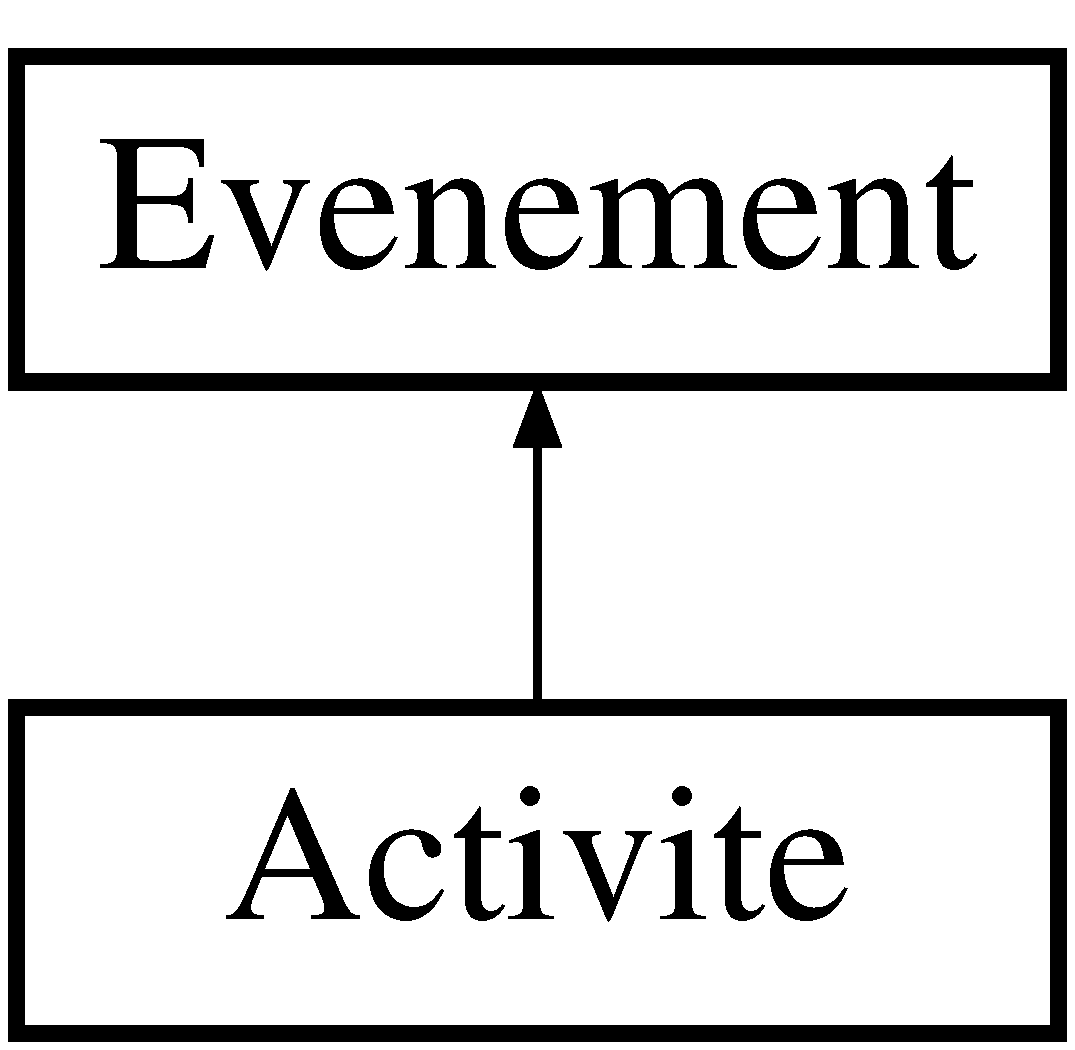
\includegraphics[height=2.000000cm]{class_activite}
\end{center}
\end{figure}
\subsection*{Types publics}
\begin{DoxyCompactItemize}
\item 
\hypertarget{class_activite_a5553b707c56acfc1dd945f47288f8a66}{}enum {\bfseries Type\+Activite} \{ {\bfseries R\+D\+V}, 
{\bfseries R\+E\+U\+N\+I\+O\+N}
 \}\label{class_activite_a5553b707c56acfc1dd945f47288f8a66}

\end{DoxyCompactItemize}
\subsection*{Fonctions membres publiques}
\begin{DoxyCompactItemize}
\item 
const Q\+String \hyperlink{class_activite_a3590379c3a3ca9576daf546839f7bd8b}{get\+Id} () const 
\item 
const Type\+Activite \& \hyperlink{class_activite_a95c674ca8775241901bc43112b253bd2}{get\+Type} () const 
\item 
Q\+String \hyperlink{class_activite_a00ba08913dad4b7e6cd47016b1ae1e83}{get\+Type\+To\+String} () const 
\item 
Q\+String \hyperlink{class_activite_a81a06135fa07489e7ed8d9363510467e}{get\+Titre} () const 
\item 
Q\+String \hyperlink{class_activite_a82dd41b3ab9c2d00848d88ea8d985743}{who\+Am\+I} () const 
\item 
bool \hyperlink{class_activite_a2d5539913a03522aa2244cf091d05aab}{is\+Preemptive} () const override
\item 
void \hyperlink{class_activite_a86514a48976df542b3ff15b1bf35003e}{set\+Id} (const Q\+String \&i)
\item 
void \hyperlink{class_activite_a8d708867c97f1eea188dce47e56ddf40}{set\+Titre} (const Q\+String \&t)
\item 
void \hyperlink{class_activite_a4fa019070cce66fbd8bcd8667a70480d}{set\+Type} (const Type\+Activite \&t)
\item 
void \hyperlink{class_activite_a519fc19bc5051e236631e14e3d564ed2}{set\+Type\+From\+String} (const Q\+String \&t)
\item 
virtual void \hyperlink{class_activite_a7643c2d88519c174143318cf8f813dc0}{afficher} () const 
\end{DoxyCompactItemize}
\subsection*{Amis}
\begin{DoxyCompactItemize}
\item 
\hypertarget{class_activite_a3e1acfebc533ba2365df5d04515154dd}{}class {\bfseries Activite\+Manager}\label{class_activite_a3e1acfebc533ba2365df5d04515154dd}

\end{DoxyCompactItemize}
\subsection*{Membres hérités additionnels}


\subsection{Description détaillée}
Une \hyperlink{class_activite}{Activite} est un évènement qui programmable. Elle ne peut être instanciée que par le biais de l\textquotesingle{}\hyperlink{class_activite_manager}{Activite\+Manager}. 

\subsection{Documentation des fonctions membres}
\hypertarget{class_activite_a7643c2d88519c174143318cf8f813dc0}{}\index{Activite@{Activite}!afficher@{afficher}}
\index{afficher@{afficher}!Activite@{Activite}}
\subsubsection[{afficher}]{\setlength{\rightskip}{0pt plus 5cm}void Activite\+::afficher (
\begin{DoxyParamCaption}
{}
\end{DoxyParamCaption}
) const\hspace{0.3cm}{\ttfamily [virtual]}}\label{class_activite_a7643c2d88519c174143318cf8f813dc0}
La méthode \hyperlink{class_activite_a7643c2d88519c174143318cf8f813dc0}{afficher()} permet d\textquotesingle{}afficher en mode debug les attributs de l\textquotesingle{}activité.\hypertarget{class_activite_a3590379c3a3ca9576daf546839f7bd8b}{}\index{Activite@{Activite}!get\+Id@{get\+Id}}
\index{get\+Id@{get\+Id}!Activite@{Activite}}
\subsubsection[{get\+Id}]{\setlength{\rightskip}{0pt plus 5cm}const Q\+String Activite\+::get\+Id (
\begin{DoxyParamCaption}
{}
\end{DoxyParamCaption}
) const\hspace{0.3cm}{\ttfamily [inline]}, {\ttfamily [virtual]}}\label{class_activite_a3590379c3a3ca9576daf546839f7bd8b}
Renvoie l\textquotesingle{}identificateur de l\textquotesingle{}activité. 

Implémente \hyperlink{class_evenement}{Evenement}.

\hypertarget{class_activite_a81a06135fa07489e7ed8d9363510467e}{}\index{Activite@{Activite}!get\+Titre@{get\+Titre}}
\index{get\+Titre@{get\+Titre}!Activite@{Activite}}
\subsubsection[{get\+Titre}]{\setlength{\rightskip}{0pt plus 5cm}Q\+String Activite\+::get\+Titre (
\begin{DoxyParamCaption}
{}
\end{DoxyParamCaption}
) const\hspace{0.3cm}{\ttfamily [inline]}}\label{class_activite_a81a06135fa07489e7ed8d9363510467e}
Renvoie le titre de l\textquotesingle{}activité. \hypertarget{class_activite_a95c674ca8775241901bc43112b253bd2}{}\index{Activite@{Activite}!get\+Type@{get\+Type}}
\index{get\+Type@{get\+Type}!Activite@{Activite}}
\subsubsection[{get\+Type}]{\setlength{\rightskip}{0pt plus 5cm}const Type\+Activite\& Activite\+::get\+Type (
\begin{DoxyParamCaption}
{}
\end{DoxyParamCaption}
) const\hspace{0.3cm}{\ttfamily [inline]}}\label{class_activite_a95c674ca8775241901bc43112b253bd2}
Renvoie le type de l\textquotesingle{}activité sous forme d\textquotesingle{}un Type\+Activite (voir énumération Type\+Activite). \hypertarget{class_activite_a00ba08913dad4b7e6cd47016b1ae1e83}{}\index{Activite@{Activite}!get\+Type\+To\+String@{get\+Type\+To\+String}}
\index{get\+Type\+To\+String@{get\+Type\+To\+String}!Activite@{Activite}}
\subsubsection[{get\+Type\+To\+String}]{\setlength{\rightskip}{0pt plus 5cm}Q\+String Activite\+::get\+Type\+To\+String (
\begin{DoxyParamCaption}
{}
\end{DoxyParamCaption}
) const\hspace{0.3cm}{\ttfamily [inline]}}\label{class_activite_a00ba08913dad4b7e6cd47016b1ae1e83}
Renvoie le type de l\textquotesingle{}activité sous forme de chaine de caractères const char$\ast$. \hypertarget{class_activite_a2d5539913a03522aa2244cf091d05aab}{}\index{Activite@{Activite}!is\+Preemptive@{is\+Preemptive}}
\index{is\+Preemptive@{is\+Preemptive}!Activite@{Activite}}
\subsubsection[{is\+Preemptive}]{\setlength{\rightskip}{0pt plus 5cm}bool Activite\+::is\+Preemptive (
\begin{DoxyParamCaption}
{}
\end{DoxyParamCaption}
) const\hspace{0.3cm}{\ttfamily [inline]}, {\ttfamily [override]}, {\ttfamily [virtual]}}\label{class_activite_a2d5539913a03522aa2244cf091d05aab}
Renvoie faux sur la premptivité de l\textquotesingle{}évènement (un activité ne peut être préemptive). 

Implémente \hyperlink{class_evenement}{Evenement}.

\hypertarget{class_activite_a86514a48976df542b3ff15b1bf35003e}{}\index{Activite@{Activite}!set\+Id@{set\+Id}}
\index{set\+Id@{set\+Id}!Activite@{Activite}}
\subsubsection[{set\+Id}]{\setlength{\rightskip}{0pt plus 5cm}void Activite\+::set\+Id (
\begin{DoxyParamCaption}
\item[{const Q\+String \&}]{i}
\end{DoxyParamCaption}
)\hspace{0.3cm}{\ttfamily [inline]}}\label{class_activite_a86514a48976df542b3ff15b1bf35003e}
Met à jour l\textquotesingle{}identificateur de l\textquotesingle{}évènement. \hypertarget{class_activite_a8d708867c97f1eea188dce47e56ddf40}{}\index{Activite@{Activite}!set\+Titre@{set\+Titre}}
\index{set\+Titre@{set\+Titre}!Activite@{Activite}}
\subsubsection[{set\+Titre}]{\setlength{\rightskip}{0pt plus 5cm}void Activite\+::set\+Titre (
\begin{DoxyParamCaption}
\item[{const Q\+String \&}]{t}
\end{DoxyParamCaption}
)\hspace{0.3cm}{\ttfamily [inline]}}\label{class_activite_a8d708867c97f1eea188dce47e56ddf40}
Met à jour le titre de l\textquotesingle{}évènement. \hypertarget{class_activite_a4fa019070cce66fbd8bcd8667a70480d}{}\index{Activite@{Activite}!set\+Type@{set\+Type}}
\index{set\+Type@{set\+Type}!Activite@{Activite}}
\subsubsection[{set\+Type}]{\setlength{\rightskip}{0pt plus 5cm}void Activite\+::set\+Type (
\begin{DoxyParamCaption}
\item[{const Type\+Activite \&}]{t}
\end{DoxyParamCaption}
)\hspace{0.3cm}{\ttfamily [inline]}}\label{class_activite_a4fa019070cce66fbd8bcd8667a70480d}
Met à jour le type de l\textquotesingle{}activité. \hypertarget{class_activite_a519fc19bc5051e236631e14e3d564ed2}{}\index{Activite@{Activite}!set\+Type\+From\+String@{set\+Type\+From\+String}}
\index{set\+Type\+From\+String@{set\+Type\+From\+String}!Activite@{Activite}}
\subsubsection[{set\+Type\+From\+String}]{\setlength{\rightskip}{0pt plus 5cm}void Activite\+::set\+Type\+From\+String (
\begin{DoxyParamCaption}
\item[{const Q\+String \&}]{t}
\end{DoxyParamCaption}
)\hspace{0.3cm}{\ttfamily [inline]}}\label{class_activite_a519fc19bc5051e236631e14e3d564ed2}
Met à jour le type de l\textquotesingle{}activité \hypertarget{class_activite_a82dd41b3ab9c2d00848d88ea8d985743}{}\index{Activite@{Activite}!who\+Am\+I@{who\+Am\+I}}
\index{who\+Am\+I@{who\+Am\+I}!Activite@{Activite}}
\subsubsection[{who\+Am\+I}]{\setlength{\rightskip}{0pt plus 5cm}Q\+String Activite\+::who\+Am\+I (
\begin{DoxyParamCaption}
{}
\end{DoxyParamCaption}
) const\hspace{0.3cm}{\ttfamily [inline]}, {\ttfamily [virtual]}}\label{class_activite_a82dd41b3ab9c2d00848d88ea8d985743}
Renvoie le type de l\textquotesingle{}évènement, ici \char`\"{}activite\char`\"{}. 

Implémente \hyperlink{class_evenement}{Evenement}.



La documentation de cette classe a été générée à partir des fichiers suivants \+:\begin{DoxyCompactItemize}
\item 
evenement.\+h\item 
evenement.\+cpp\end{DoxyCompactItemize}

\hypertarget{class_activite_manager}{}\section{Référence de la classe Activite\+Manager}
\label{class_activite_manager}\index{Activite\+Manager@{Activite\+Manager}}


La classe \hyperlink{class_activite_manager}{Activite\+Manager} est un \hyperlink{class_manager}{Manager} qui gère les items de type activité. Elle ne peut être instanciée à cause du singleton mis en place dans sa classe mère. Elle peut toutefois être récupérée dans une référence ou un pointeur à l\textquotesingle{}aide la méthode mère\+: \hyperlink{class_manager_a8372e4f1e14f3605a57d839b152325ed}{get\+Instance()}.  




{\ttfamily \#include $<$manager.\+h$>$}

Graphe d\textquotesingle{}héritage de Activite\+Manager\+:\begin{figure}[H]
\begin{center}
\leavevmode
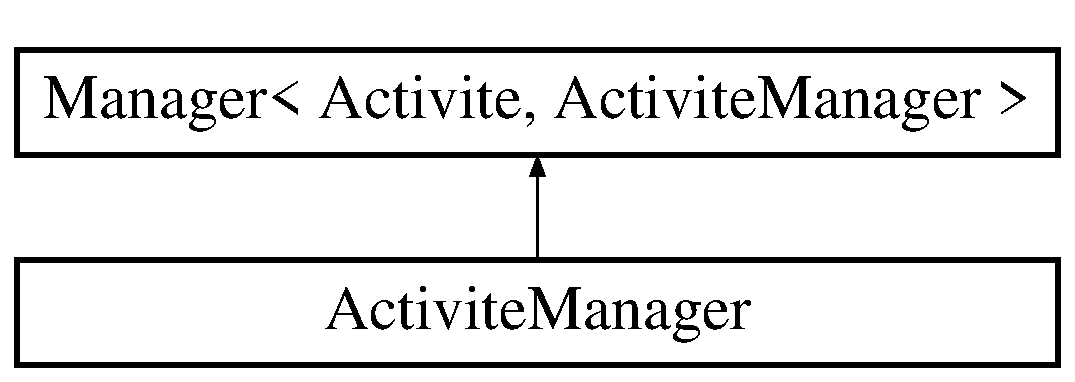
\includegraphics[height=2.000000cm]{class_activite_manager}
\end{center}
\end{figure}
\subsection*{Fonctions membres publiques}
\begin{DoxyCompactItemize}
\item 
\hyperlink{class_activite}{Activite} \& \hyperlink{class_activite_manager_a6c62c6f427c541d44c8da3eef994e562}{ajouter\+Activite} (const Q\+String \&id, const Q\+String \&t, const Activite\+::\+Type\+Activite \&ty, const \hyperlink{class_q_time_span}{Q\+Time\+Span} \&d)
\item 
\hyperlink{class_activite}{Activite} \& \hyperlink{class_activite_manager_a275464cd4fd5b3ca57dfeb10120146d0}{ajouter\+Activite} (const Q\+String \&id, const Q\+String \&t, const Activite\+::\+Type\+Activite \&ty, const Q\+String \&d)
\end{DoxyCompactItemize}
\subsection*{Membres hérités additionnels}


\subsection{Description détaillée}
La classe \hyperlink{class_activite_manager}{Activite\+Manager} est un \hyperlink{class_manager}{Manager} qui gère les items de type activité. Elle ne peut être instanciée à cause du singleton mis en place dans sa classe mère. Elle peut toutefois être récupérée dans une référence ou un pointeur à l\textquotesingle{}aide la méthode mère\+: \hyperlink{class_manager_a8372e4f1e14f3605a57d839b152325ed}{get\+Instance()}. 

\subsection{Documentation des fonctions membres}
\hypertarget{class_activite_manager_a6c62c6f427c541d44c8da3eef994e562}{}\index{Activite\+Manager@{Activite\+Manager}!ajouter\+Activite@{ajouter\+Activite}}
\index{ajouter\+Activite@{ajouter\+Activite}!Activite\+Manager@{Activite\+Manager}}
\subsubsection[{ajouter\+Activite}]{\setlength{\rightskip}{0pt plus 5cm}{\bf Activite} \& Activite\+Manager\+::ajouter\+Activite (
\begin{DoxyParamCaption}
\item[{const Q\+String \&}]{id, }
\item[{const Q\+String \&}]{t, }
\item[{const Activite\+::\+Type\+Activite \&}]{ty, }
\item[{const {\bf Q\+Time\+Span} \&}]{d}
\end{DoxyParamCaption}
)}\label{class_activite_manager_a6c62c6f427c541d44c8da3eef994e562}
Créer une activité en vérifiant les attributs passés en paramètre. Puis l\textquotesingle{}ajoute au vecteur et renvoie sa référence. \hypertarget{class_activite_manager_a275464cd4fd5b3ca57dfeb10120146d0}{}\index{Activite\+Manager@{Activite\+Manager}!ajouter\+Activite@{ajouter\+Activite}}
\index{ajouter\+Activite@{ajouter\+Activite}!Activite\+Manager@{Activite\+Manager}}
\subsubsection[{ajouter\+Activite}]{\setlength{\rightskip}{0pt plus 5cm}{\bf Activite} \& Activite\+Manager\+::ajouter\+Activite (
\begin{DoxyParamCaption}
\item[{const Q\+String \&}]{id, }
\item[{const Q\+String \&}]{t, }
\item[{const Activite\+::\+Type\+Activite \&}]{ty, }
\item[{const Q\+String \&}]{d}
\end{DoxyParamCaption}
)}\label{class_activite_manager_a275464cd4fd5b3ca57dfeb10120146d0}
Créer une activité en vérifiant les attributs passés en paramètre. Puis l\textquotesingle{}ajoute au vecteur et renvoie sa référence. 

La documentation de cette classe a été générée à partir des fichiers suivants \+:\begin{DoxyCompactItemize}
\item 
manager.\+h\item 
manager.\+cpp\end{DoxyCompactItemize}

\hypertarget{classajouter_activite}{}\section{Référence de la classe ajouter\+Activite}
\label{classajouter_activite}\index{ajouter\+Activite@{ajouter\+Activite}}


Fenêtre d\textquotesingle{}ajout et de modification d\textquotesingle{}\hyperlink{class_activite}{Activite}.  




{\ttfamily \#include $<$ajouteractivite.\+h$>$}

Graphe d\textquotesingle{}héritage de ajouter\+Activite\+:\begin{figure}[H]
\begin{center}
\leavevmode
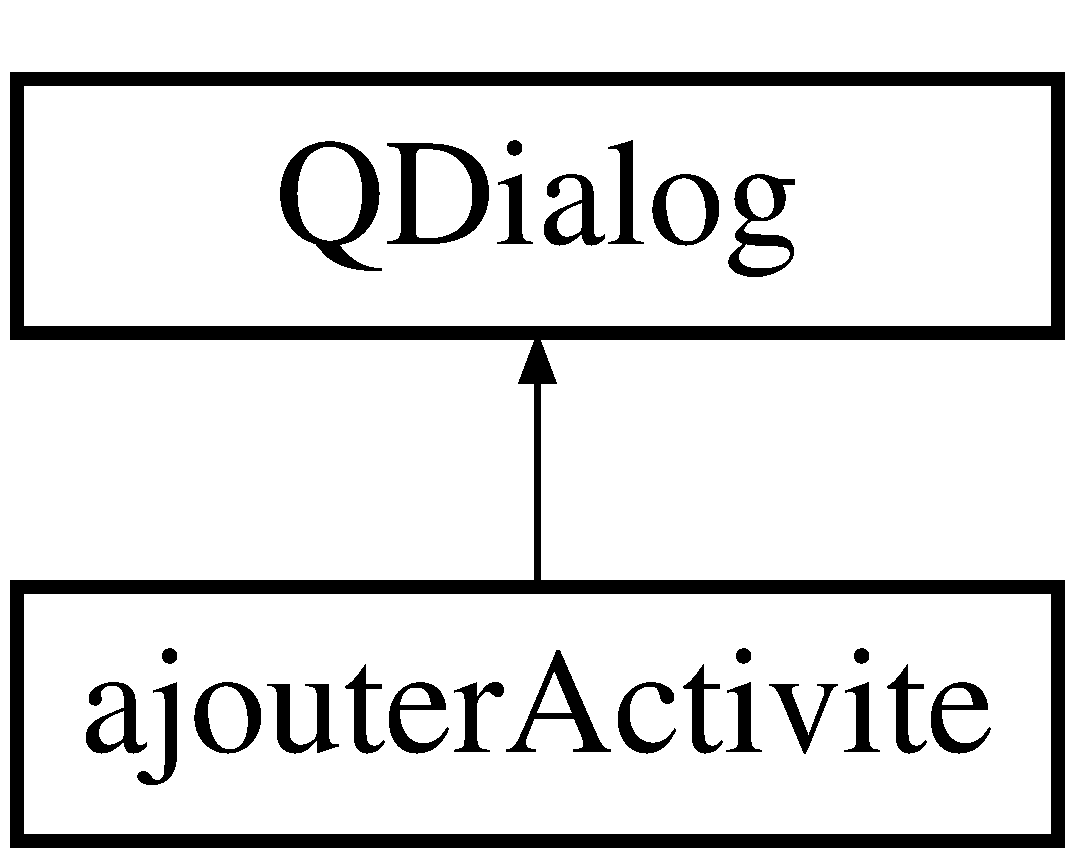
\includegraphics[height=2.000000cm]{classajouter_activite}
\end{center}
\end{figure}
\subsection*{Fonctions membres publiques}
\begin{DoxyCompactItemize}
\item 
\hypertarget{classajouter_activite_af65ef144a5efeed204f428d77dfb2418}{}{\bfseries ajouter\+Activite} (\hyperlink{class_activite}{Activite} $\ast$activite=0, Q\+Widget $\ast$parent=0)\label{classajouter_activite_af65ef144a5efeed204f428d77dfb2418}

\end{DoxyCompactItemize}


\subsection{Description détaillée}
Fenêtre d\textquotesingle{}ajout et de modification d\textquotesingle{}\hyperlink{class_activite}{Activite}. 

La documentation de cette classe a été générée à partir des fichiers suivants \+:\begin{DoxyCompactItemize}
\item 
G\+U\+I/ajouteractivite.\+h\item 
G\+U\+I/ajouteractivite.\+cpp\end{DoxyCompactItemize}

\hypertarget{classajouter_projet}{}\section{Référence de la classe ajouter\+Projet}
\label{classajouter_projet}\index{ajouter\+Projet@{ajouter\+Projet}}


Fenêtre d\textquotesingle{}ajout et de modification de \hyperlink{class_projet}{Projet}.  




{\ttfamily \#include $<$ajouterprojet.\+h$>$}

Graphe d\textquotesingle{}héritage de ajouter\+Projet\+:\begin{figure}[H]
\begin{center}
\leavevmode
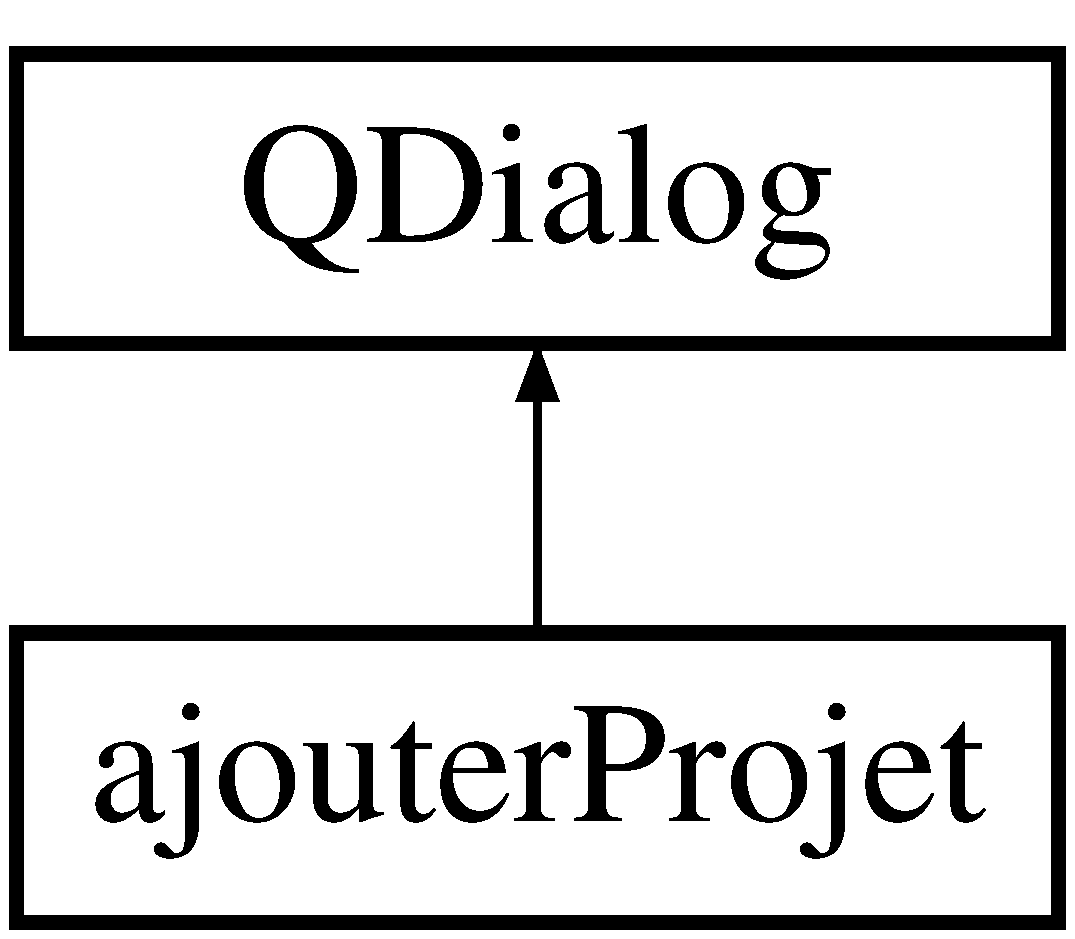
\includegraphics[height=2.000000cm]{classajouter_projet}
\end{center}
\end{figure}
\subsection*{Fonctions membres publiques}
\begin{DoxyCompactItemize}
\item 
\hypertarget{classajouter_projet_a8d01a20eb1e6ee26473468edc1139fee}{}{\bfseries ajouter\+Projet} (\hyperlink{class_projet}{Projet} $\ast$projet=0, Q\+Widget $\ast$parent=0)\label{classajouter_projet_a8d01a20eb1e6ee26473468edc1139fee}

\end{DoxyCompactItemize}


\subsection{Description détaillée}
Fenêtre d\textquotesingle{}ajout et de modification de \hyperlink{class_projet}{Projet}. 

La documentation de cette classe a été générée à partir des fichiers suivants \+:\begin{DoxyCompactItemize}
\item 
G\+U\+I/ajouterprojet.\+h\item 
G\+U\+I/ajouterprojet.\+cpp\end{DoxyCompactItemize}

\hypertarget{classajouter_tache_composite}{}\section{Référence de la classe ajouter\+Tache\+Composite}
\label{classajouter_tache_composite}\index{ajouter\+Tache\+Composite@{ajouter\+Tache\+Composite}}


Fenêtre d\textquotesingle{}ajout et de modification de \hyperlink{class_tache_composite}{Tache\+Composite}.  




{\ttfamily \#include $<$ajoutertachecomposite.\+h$>$}

Graphe d\textquotesingle{}héritage de ajouter\+Tache\+Composite\+:\begin{figure}[H]
\begin{center}
\leavevmode
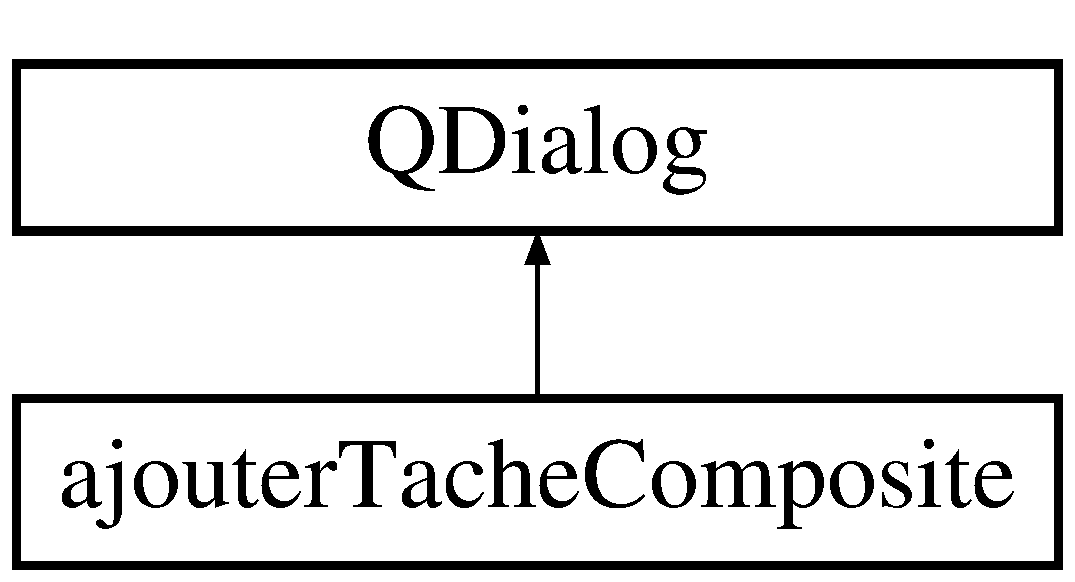
\includegraphics[height=2.000000cm]{classajouter_tache_composite}
\end{center}
\end{figure}
\subsection*{Fonctions membres publiques}
\begin{DoxyCompactItemize}
\item 
\hypertarget{classajouter_tache_composite_a831093adfc82d73e96e81d37b88d9a9b}{}{\bfseries ajouter\+Tache\+Composite} (\hyperlink{class_tache_composite}{Tache\+Composite} $\ast$tache=0, Q\+Widget $\ast$parent=0)\label{classajouter_tache_composite_a831093adfc82d73e96e81d37b88d9a9b}

\end{DoxyCompactItemize}


\subsection{Description détaillée}
Fenêtre d\textquotesingle{}ajout et de modification de \hyperlink{class_tache_composite}{Tache\+Composite}. 

La documentation de cette classe a été générée à partir des fichiers suivants \+:\begin{DoxyCompactItemize}
\item 
G\+U\+I/ajoutertachecomposite.\+h\item 
G\+U\+I/ajoutertachecomposite.\+cpp\end{DoxyCompactItemize}

\hypertarget{class_tache_composite_1_1const__iterator}{}\section{Référence de la classe Tache\+Composite\+:\+:const\+\_\+iterator}
\label{class_tache_composite_1_1const__iterator}\index{Tache\+Composite\+::const\+\_\+iterator@{Tache\+Composite\+::const\+\_\+iterator}}
Graphe d\textquotesingle{}héritage de Tache\+Composite\+:\+:const\+\_\+iterator\+:\begin{figure}[H]
\begin{center}
\leavevmode
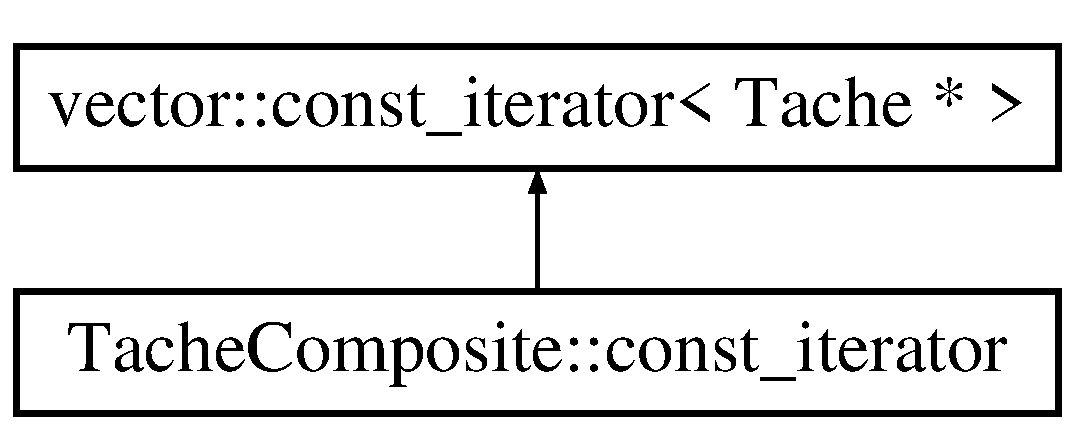
\includegraphics[height=2.000000cm]{class_tache_composite_1_1const__iterator}
\end{center}
\end{figure}
\subsection*{Fonctions membres publiques}
\begin{DoxyCompactItemize}
\item 
\hypertarget{class_tache_composite_1_1const__iterator_a674fb157f64fa34cc4194e3e59afdfcc}{}{\bfseries const\+\_\+iterator} (vector$<$ \hyperlink{class_tache}{Tache} $\ast$ $>$\+::\hyperlink{class_tache_composite_1_1const__iterator}{const\+\_\+iterator} it)\label{class_tache_composite_1_1const__iterator_a674fb157f64fa34cc4194e3e59afdfcc}

\end{DoxyCompactItemize}


La documentation de cette classe a été générée à partir du fichier suivant \+:\begin{DoxyCompactItemize}
\item 
evenement.\+h\end{DoxyCompactItemize}

\hypertarget{class_projet_1_1const__iterator}{}\section{Référence de la classe Projet\+:\+:const\+\_\+iterator}
\label{class_projet_1_1const__iterator}\index{Projet\+::const\+\_\+iterator@{Projet\+::const\+\_\+iterator}}
Graphe d\textquotesingle{}héritage de Projet\+:\+:const\+\_\+iterator\+:\begin{figure}[H]
\begin{center}
\leavevmode
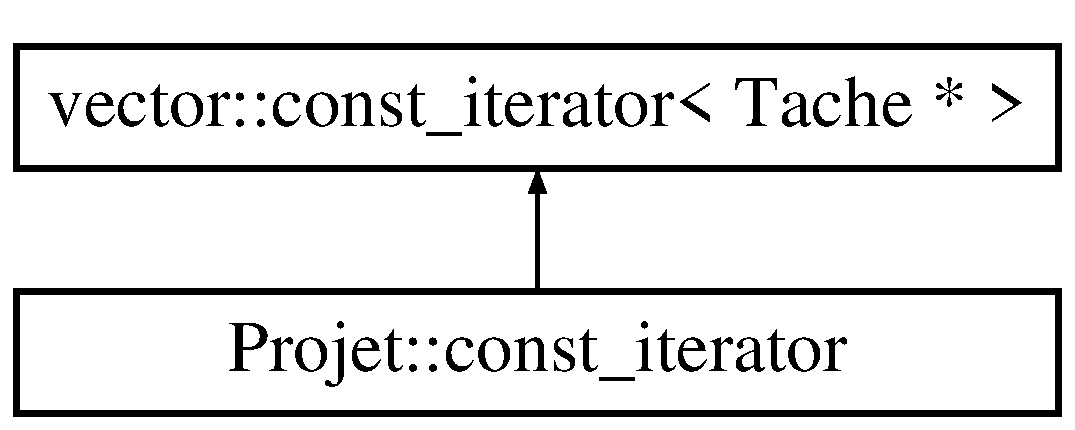
\includegraphics[height=2.000000cm]{class_projet_1_1const__iterator}
\end{center}
\end{figure}
\subsection*{Fonctions membres publiques}
\begin{DoxyCompactItemize}
\item 
\hypertarget{class_projet_1_1const__iterator_adec014c18cd3419ac3302c9a47dd88e2}{}{\bfseries const\+\_\+iterator} (vector$<$ \hyperlink{class_tache}{Tache} $\ast$ $>$\+::\hyperlink{class_projet_1_1const__iterator}{const\+\_\+iterator} it)\label{class_projet_1_1const__iterator_adec014c18cd3419ac3302c9a47dd88e2}

\end{DoxyCompactItemize}


La documentation de cette classe a été générée à partir du fichier suivant \+:\begin{DoxyCompactItemize}
\item 
evenement.\+h\end{DoxyCompactItemize}

\hypertarget{class_manager_1_1const__iterator}{}\section{Référence de la classe Manager$<$ T, U $>$\+:\+:const\+\_\+iterator}
\label{class_manager_1_1const__iterator}\index{Manager$<$ T, U $>$\+::const\+\_\+iterator@{Manager$<$ T, U $>$\+::const\+\_\+iterator}}
Graphe d\textquotesingle{}héritage de Manager$<$ T, U $>$\+:\+:const\+\_\+iterator\+:\begin{figure}[H]
\begin{center}
\leavevmode
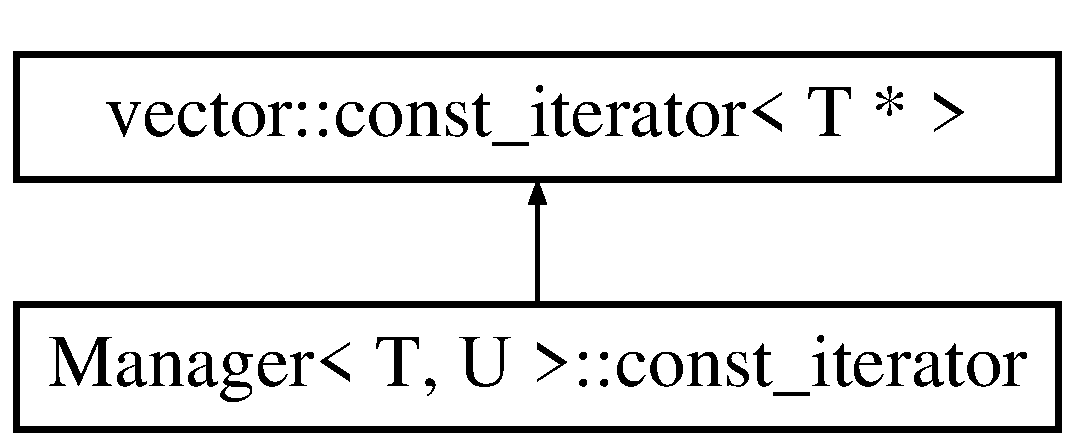
\includegraphics[height=2.000000cm]{class_manager_1_1const__iterator}
\end{center}
\end{figure}
\subsection*{Fonctions membres publiques}
\begin{DoxyCompactItemize}
\item 
\hypertarget{class_manager_1_1const__iterator_a0b291f291404f06dac59623886f02424}{}{\bfseries const\+\_\+iterator} (typename vector$<$ T $\ast$ $>$\+::\hyperlink{class_manager_1_1const__iterator}{const\+\_\+iterator} it)\label{class_manager_1_1const__iterator_a0b291f291404f06dac59623886f02424}

\end{DoxyCompactItemize}


La documentation de cette classe a été générée à partir du fichier suivant \+:\begin{DoxyCompactItemize}
\item 
manager.\+h\end{DoxyCompactItemize}

\hypertarget{class_t_i_m_e_1_1_date}{}\section{Référence de la classe T\+I\+M\+E\+:\+:Date}
\label{class_t_i_m_e_1_1_date}\index{T\+I\+M\+E\+::\+Date@{T\+I\+M\+E\+::\+Date}}


Classe permettant de manipuler des dates standards L\textquotesingle{}utilisation de cette classe nécessite des dates valides au sens commun du terme. Déclenchement d\textquotesingle{}exception dans le cas contraire.  




{\ttfamily \#include $<$timing.\+h$>$}

\subsection*{Fonctions membres publiques}
\begin{DoxyCompactItemize}
\item 
\hyperlink{class_t_i_m_e_1_1_date_ab0d72ce6e986c0c0a5f2902e586cf81a}{Date} (unsigned int short j=1, unsigned int short m=1, unsigned int a=0)
\begin{DoxyCompactList}\small\item\em Constructeur à partir d\textquotesingle{}un jour, mois, année. \end{DoxyCompactList}\item 
\hypertarget{class_t_i_m_e_1_1_date_a4af978b7df2b738f62449b0a7e53c21d}{}unsigned short int {\bfseries get\+Jour} () const \label{class_t_i_m_e_1_1_date_a4af978b7df2b738f62449b0a7e53c21d}

\item 
\hypertarget{class_t_i_m_e_1_1_date_a6cb9d945143df216115419c4cb8b14ce}{}unsigned short int {\bfseries get\+Mois} () const \label{class_t_i_m_e_1_1_date_a6cb9d945143df216115419c4cb8b14ce}

\item 
\hypertarget{class_t_i_m_e_1_1_date_a07b41b2e9e85ef78bf13689e772bef7d}{}unsigned int {\bfseries get\+Annee} () const \label{class_t_i_m_e_1_1_date_a07b41b2e9e85ef78bf13689e772bef7d}

\item 
\hypertarget{class_t_i_m_e_1_1_date_a7419902750e61b9473ab05ccd5ced33d}{}void \hyperlink{class_t_i_m_e_1_1_date_a7419902750e61b9473ab05ccd5ced33d}{set\+Date} (unsigned short int j, unsigned short int m, unsigned int a)\label{class_t_i_m_e_1_1_date_a7419902750e61b9473ab05ccd5ced33d}

\begin{DoxyCompactList}\small\item\em initialisation de la date \end{DoxyCompactList}\item 
\hypertarget{class_t_i_m_e_1_1_date_ace4be52a503c45de93b8db92dc592d93}{}void \hyperlink{class_t_i_m_e_1_1_date_ace4be52a503c45de93b8db92dc592d93}{set\+Date\+Aujourdhui} ()\label{class_t_i_m_e_1_1_date_ace4be52a503c45de93b8db92dc592d93}

\begin{DoxyCompactList}\small\item\em initialisation de la date avec la date d\textquotesingle{}aujourd\textquotesingle{}hui \end{DoxyCompactList}\item 
\hypertarget{class_t_i_m_e_1_1_date_aa45188755f5d9d17cbebf0e55d3c571b}{}void \hyperlink{class_t_i_m_e_1_1_date_aa45188755f5d9d17cbebf0e55d3c571b}{afficher} (std\+::ostream \&f=std\+::cout) const \label{class_t_i_m_e_1_1_date_aa45188755f5d9d17cbebf0e55d3c571b}

\begin{DoxyCompactList}\small\item\em affiche le date sous le format J\+J/\+M\+M/\+A\+A\+A\+A \end{DoxyCompactList}\item 
\hypertarget{class_t_i_m_e_1_1_date_aa8208298c0efe5dbf661c66a284fd163}{}bool {\bfseries operator==} (const \hyperlink{class_t_i_m_e_1_1_date}{Date} \&d) const \label{class_t_i_m_e_1_1_date_aa8208298c0efe5dbf661c66a284fd163}

\item 
\hypertarget{class_t_i_m_e_1_1_date_a8a3bccb05f00086e64c5b5518a37949f}{}bool {\bfseries operator$<$} (const \hyperlink{class_t_i_m_e_1_1_date}{Date} \&d) const \label{class_t_i_m_e_1_1_date_a8a3bccb05f00086e64c5b5518a37949f}

\item 
\hypertarget{class_t_i_m_e_1_1_date_a61f93f8612a998bc440070f9b8a2660a}{}int {\bfseries operator-\/} (const \hyperlink{class_t_i_m_e_1_1_date}{Date} \&d) const \label{class_t_i_m_e_1_1_date_a61f93f8612a998bc440070f9b8a2660a}

\item 
\hypertarget{class_t_i_m_e_1_1_date_a85907da4cadaff930c748328fda4d527}{}\hyperlink{class_t_i_m_e_1_1_date}{Date} {\bfseries demain} () const \label{class_t_i_m_e_1_1_date_a85907da4cadaff930c748328fda4d527}

\item 
\hypertarget{class_t_i_m_e_1_1_date_a3c1f346c2ad9287155a71dc5d09e7fd8}{}\hyperlink{class_t_i_m_e_1_1_date}{Date} {\bfseries operator+} (unsigned int nb) const \label{class_t_i_m_e_1_1_date_a3c1f346c2ad9287155a71dc5d09e7fd8}

\end{DoxyCompactItemize}


\subsection{Description détaillée}
Classe permettant de manipuler des dates standards L\textquotesingle{}utilisation de cette classe nécessite des dates valides au sens commun du terme. Déclenchement d\textquotesingle{}exception dans le cas contraire. 

\subsection{Documentation des constructeurs et destructeur}
\hypertarget{class_t_i_m_e_1_1_date_ab0d72ce6e986c0c0a5f2902e586cf81a}{}\index{T\+I\+M\+E\+::\+Date@{T\+I\+M\+E\+::\+Date}!Date@{Date}}
\index{Date@{Date}!T\+I\+M\+E\+::\+Date@{T\+I\+M\+E\+::\+Date}}
\subsubsection[{Date}]{\setlength{\rightskip}{0pt plus 5cm}T\+I\+M\+E\+::\+Date\+::\+Date (
\begin{DoxyParamCaption}
\item[{unsigned int short}]{j = {\ttfamily 1}, }
\item[{unsigned int short}]{m = {\ttfamily 1}, }
\item[{unsigned int}]{a = {\ttfamily 0}}
\end{DoxyParamCaption}
)\hspace{0.3cm}{\ttfamily [inline]}}\label{class_t_i_m_e_1_1_date_ab0d72ce6e986c0c0a5f2902e586cf81a}


Constructeur à partir d\textquotesingle{}un jour, mois, année. 


\begin{DoxyParams}{Paramètres}
{\em j} & jour avec 1$<$=j$<$=31 \\
\hline
{\em m} & mois avec 1$<$=m$<$=12 \\
\hline
{\em a} & année avec a$>$=0 \\
\hline
\end{DoxyParams}


La documentation de cette classe a été générée à partir des fichiers suivants \+:\begin{DoxyCompactItemize}
\item 
timing.\+h\item 
timing.\+cpp\end{DoxyCompactItemize}

\hypertarget{class_t_i_m_e_1_1_duree}{}\section{Référence de la classe T\+I\+M\+E\+:\+:Duree}
\label{class_t_i_m_e_1_1_duree}\index{T\+I\+M\+E\+::\+Duree@{T\+I\+M\+E\+::\+Duree}}


Classe permettant de manipuler des durees L\textquotesingle{}utilisation de cette classe nécessite des dates valides au sens commun du terme. Déclenchement d\textquotesingle{}exception dans le cas contraire.  




{\ttfamily \#include $<$timing.\+h$>$}

\subsection*{Fonctions membres publiques}
\begin{DoxyCompactItemize}
\item 
\hyperlink{class_t_i_m_e_1_1_duree_ae0532a0d60dbc31773f038967dfe220e}{Duree} (unsigned int h, unsigned int m)
\begin{DoxyCompactList}\small\item\em Constructeur à partir de heure et minute. \end{DoxyCompactList}\item 
\hyperlink{class_t_i_m_e_1_1_duree_a0f99878e52fad2f9e0643301c70d9ef7}{Duree} (unsigned int m=0)
\begin{DoxyCompactList}\small\item\em Constructeur à partir de minute. \end{DoxyCompactList}\item 
\hypertarget{class_t_i_m_e_1_1_duree_aabba3e357861f21faa8419339f7b7176}{}void {\bfseries set\+Duree} (unsigned int heures, unsigned int minutes)\label{class_t_i_m_e_1_1_duree_aabba3e357861f21faa8419339f7b7176}

\item 
\hypertarget{class_t_i_m_e_1_1_duree_a1e47fb5f0734ec562e2f9dba32db45f4}{}unsigned int {\bfseries get\+Duree\+En\+Minutes} () const \label{class_t_i_m_e_1_1_duree_a1e47fb5f0734ec562e2f9dba32db45f4}

\item 
\hypertarget{class_t_i_m_e_1_1_duree_afb11d106fc1f6761a68f486dc7a17564}{}double {\bfseries get\+Duree\+En\+Heures} () const \label{class_t_i_m_e_1_1_duree_afb11d106fc1f6761a68f486dc7a17564}

\item 
\hypertarget{class_t_i_m_e_1_1_duree_ad957a58f8bc103857f3e494bab5f60e1}{}void {\bfseries afficher} (std\+::ostream \&f=std\+::cout) const \label{class_t_i_m_e_1_1_duree_ad957a58f8bc103857f3e494bab5f60e1}

\end{DoxyCompactItemize}


\subsection{Description détaillée}
Classe permettant de manipuler des durees L\textquotesingle{}utilisation de cette classe nécessite des dates valides au sens commun du terme. Déclenchement d\textquotesingle{}exception dans le cas contraire. 

\subsection{Documentation des constructeurs et destructeur}
\hypertarget{class_t_i_m_e_1_1_duree_ae0532a0d60dbc31773f038967dfe220e}{}\index{T\+I\+M\+E\+::\+Duree@{T\+I\+M\+E\+::\+Duree}!Duree@{Duree}}
\index{Duree@{Duree}!T\+I\+M\+E\+::\+Duree@{T\+I\+M\+E\+::\+Duree}}
\subsubsection[{Duree}]{\setlength{\rightskip}{0pt plus 5cm}T\+I\+M\+E\+::\+Duree\+::\+Duree (
\begin{DoxyParamCaption}
\item[{unsigned int}]{h, }
\item[{unsigned int}]{m}
\end{DoxyParamCaption}
)\hspace{0.3cm}{\ttfamily [inline]}}\label{class_t_i_m_e_1_1_duree_ae0532a0d60dbc31773f038967dfe220e}


Constructeur à partir de heure et minute. 


\begin{DoxyParams}{Paramètres}
{\em h} & heure avec h$>$=0 \\
\hline
{\em m} & minute avec 0$<$=m$<$=59 \\
\hline
\end{DoxyParams}
\hypertarget{class_t_i_m_e_1_1_duree_a0f99878e52fad2f9e0643301c70d9ef7}{}\index{T\+I\+M\+E\+::\+Duree@{T\+I\+M\+E\+::\+Duree}!Duree@{Duree}}
\index{Duree@{Duree}!T\+I\+M\+E\+::\+Duree@{T\+I\+M\+E\+::\+Duree}}
\subsubsection[{Duree}]{\setlength{\rightskip}{0pt plus 5cm}T\+I\+M\+E\+::\+Duree\+::\+Duree (
\begin{DoxyParamCaption}
\item[{unsigned int}]{m = {\ttfamily 0}}
\end{DoxyParamCaption}
)\hspace{0.3cm}{\ttfamily [inline]}}\label{class_t_i_m_e_1_1_duree_a0f99878e52fad2f9e0643301c70d9ef7}


Constructeur à partir de minute. 


\begin{DoxyParams}{Paramètres}
{\em m} & minute avec m$>$=0 \\
\hline
\end{DoxyParams}


La documentation de cette classe a été générée à partir du fichier suivant \+:\begin{DoxyCompactItemize}
\item 
timing.\+h\end{DoxyCompactItemize}

\hypertarget{class_evenement}{}\section{Référence de la classe Evenement}
\label{class_evenement}\index{Evenement@{Evenement}}


La classe \hyperlink{class_evenement}{Evenement} est virtuelle pure, seules ses classes filles\+: \hyperlink{class_tache_unitaire}{Tache\+Unitaire} et \hyperlink{class_activite}{Activite} peuvent être instanciées, par leurs Managers respectifs.  




{\ttfamily \#include $<$evenement.\+h$>$}

Graphe d\textquotesingle{}héritage de Evenement\+:\begin{figure}[H]
\begin{center}
\leavevmode
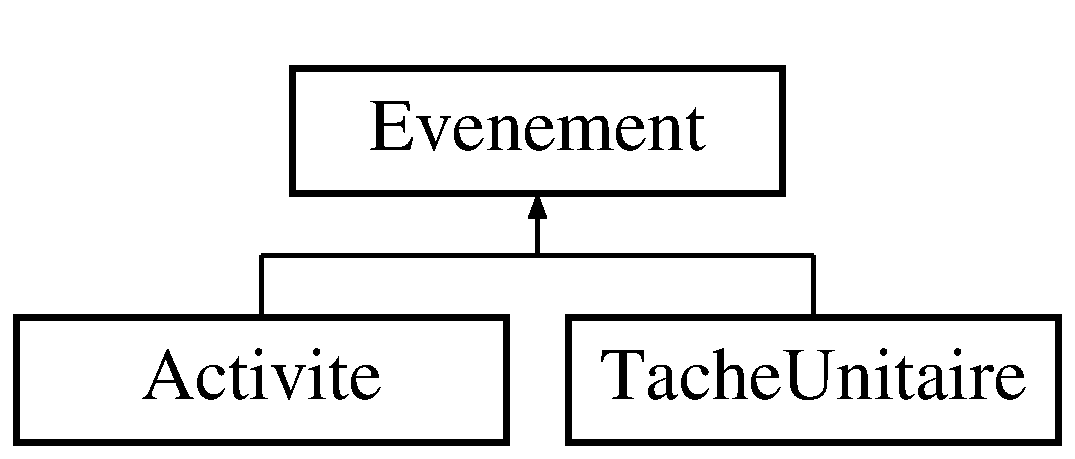
\includegraphics[height=2.000000cm]{class_evenement}
\end{center}
\end{figure}
\subsection*{Fonctions membres publiques}
\begin{DoxyCompactItemize}
\item 
const \hyperlink{class_q_time_span}{Q\+Time\+Span} \& \hyperlink{class_evenement_aec0228042f3cfe8ec970ddcbbaa57dd8}{get\+Duree} () const 
\item 
virtual void \hyperlink{class_evenement_a8e7e4eb2ec7352a1bf5a63df42c193c6}{set\+Duree} (const \hyperlink{class_q_time_span}{Q\+Time\+Span} \&d)
\item 
vector$<$ \hyperlink{class_programmation}{Programmation} $\ast$ $>$ \hyperlink{class_evenement_a5f451f67822905b35adf6c089b1f8aef}{get\+Programmations} () const 
\item 
\hypertarget{class_evenement_ace9b05926d5866254293a8a295f98e0d}{}virtual Q\+String {\bfseries who\+Am\+I} () const =0\label{class_evenement_ace9b05926d5866254293a8a295f98e0d}

\item 
\hypertarget{class_evenement_a941fd5fed58174df6cc2675306c80db7}{}virtual bool {\bfseries is\+Preemptive} () const =0\label{class_evenement_a941fd5fed58174df6cc2675306c80db7}

\item 
\hypertarget{class_evenement_a8230234b16a5056d7ec222ae79869770}{}virtual const Q\+String {\bfseries get\+Id} () const =0\label{class_evenement_a8230234b16a5056d7ec222ae79869770}

\end{DoxyCompactItemize}
\subsection*{Fonctions membres protégées}
\begin{DoxyCompactItemize}
\item 
\hypertarget{class_evenement_a4e94a42964ecbdd8eebeb25bc07b0cbb}{}{\bfseries Evenement} (const \hyperlink{class_q_time_span}{Q\+Time\+Span} \&d)\label{class_evenement_a4e94a42964ecbdd8eebeb25bc07b0cbb}

\end{DoxyCompactItemize}


\subsection{Description détaillée}
La classe \hyperlink{class_evenement}{Evenement} est virtuelle pure, seules ses classes filles\+: \hyperlink{class_tache_unitaire}{Tache\+Unitaire} et \hyperlink{class_activite}{Activite} peuvent être instanciées, par leurs Managers respectifs. 

\subsection{Documentation des fonctions membres}
\hypertarget{class_evenement_aec0228042f3cfe8ec970ddcbbaa57dd8}{}\index{Evenement@{Evenement}!get\+Duree@{get\+Duree}}
\index{get\+Duree@{get\+Duree}!Evenement@{Evenement}}
\subsubsection[{get\+Duree}]{\setlength{\rightskip}{0pt plus 5cm}const {\bf Q\+Time\+Span}\& Evenement\+::get\+Duree (
\begin{DoxyParamCaption}
{}
\end{DoxyParamCaption}
) const\hspace{0.3cm}{\ttfamily [inline]}}\label{class_evenement_aec0228042f3cfe8ec970ddcbbaa57dd8}
La méthode \hyperlink{class_evenement_aec0228042f3cfe8ec970ddcbbaa57dd8}{get\+Duree()} renvoie la durée de l\textquotesingle{}évènement. \hypertarget{class_evenement_a5f451f67822905b35adf6c089b1f8aef}{}\index{Evenement@{Evenement}!get\+Programmations@{get\+Programmations}}
\index{get\+Programmations@{get\+Programmations}!Evenement@{Evenement}}
\subsubsection[{get\+Programmations}]{\setlength{\rightskip}{0pt plus 5cm}vector$<$ {\bf Programmation} $\ast$ $>$ Evenement\+::get\+Programmations (
\begin{DoxyParamCaption}
{}
\end{DoxyParamCaption}
) const}\label{class_evenement_a5f451f67822905b35adf6c089b1f8aef}
La méthode \hyperlink{class_evenement_a5f451f67822905b35adf6c089b1f8aef}{get\+Programmations()} renvoie un vecteur de pointeurs sur les éventuelles programmations de l\textquotesingle{}évènement.
\begin{DoxyItemize}
\item Si ce dernier n\textquotesingle{}a pas été programmé, un vecteur vide sera retourné.
\item Egalement, si une tâche préemptive appelle cette méthode, plusieurs pointeurs de programmation sont susceptibles d\textquotesingle{}être retournés au sein du vecteur.
\item Sinon un seul pointeur de programmation sera retourné dans le vecteur.
\end{DoxyItemize}\hypertarget{class_evenement_a8e7e4eb2ec7352a1bf5a63df42c193c6}{}\index{Evenement@{Evenement}!set\+Duree@{set\+Duree}}
\index{set\+Duree@{set\+Duree}!Evenement@{Evenement}}
\subsubsection[{set\+Duree}]{\setlength{\rightskip}{0pt plus 5cm}virtual void Evenement\+::set\+Duree (
\begin{DoxyParamCaption}
\item[{const {\bf Q\+Time\+Span} \&}]{d}
\end{DoxyParamCaption}
)\hspace{0.3cm}{\ttfamily [inline]}, {\ttfamily [virtual]}}\label{class_evenement_a8e7e4eb2ec7352a1bf5a63df42c193c6}
La méthode \hyperlink{class_evenement_a8e7e4eb2ec7352a1bf5a63df42c193c6}{set\+Duree()} met à jour la durée avec celle passée en paramètre. 

Réimplémentée dans \hyperlink{class_tache_unitaire_a4065892def718cee931fe8bdbafa7ffc}{Tache\+Unitaire}.



La documentation de cette classe a été générée à partir des fichiers suivants \+:\begin{DoxyCompactItemize}
\item 
evenement.\+h\item 
evenement.\+cpp\end{DoxyCompactItemize}

\hypertarget{class_format}{}\section{Référence de la classe Format}
\label{class_format}\index{Format@{Format}}


\hyperlink{class_format}{Format} est une classe virtuelle pure permettant la mise en place du pattern design Strategy. Les classes fillent qui en héritent peuvent alors être utiliser par le \hyperlink{class_memento}{Memento} afin de réaliser divers types d\textquotesingle{}exportations.  




{\ttfamily \#include $<$import-\/export.\+h$>$}

Graphe d\textquotesingle{}héritage de Format\+:\begin{figure}[H]
\begin{center}
\leavevmode
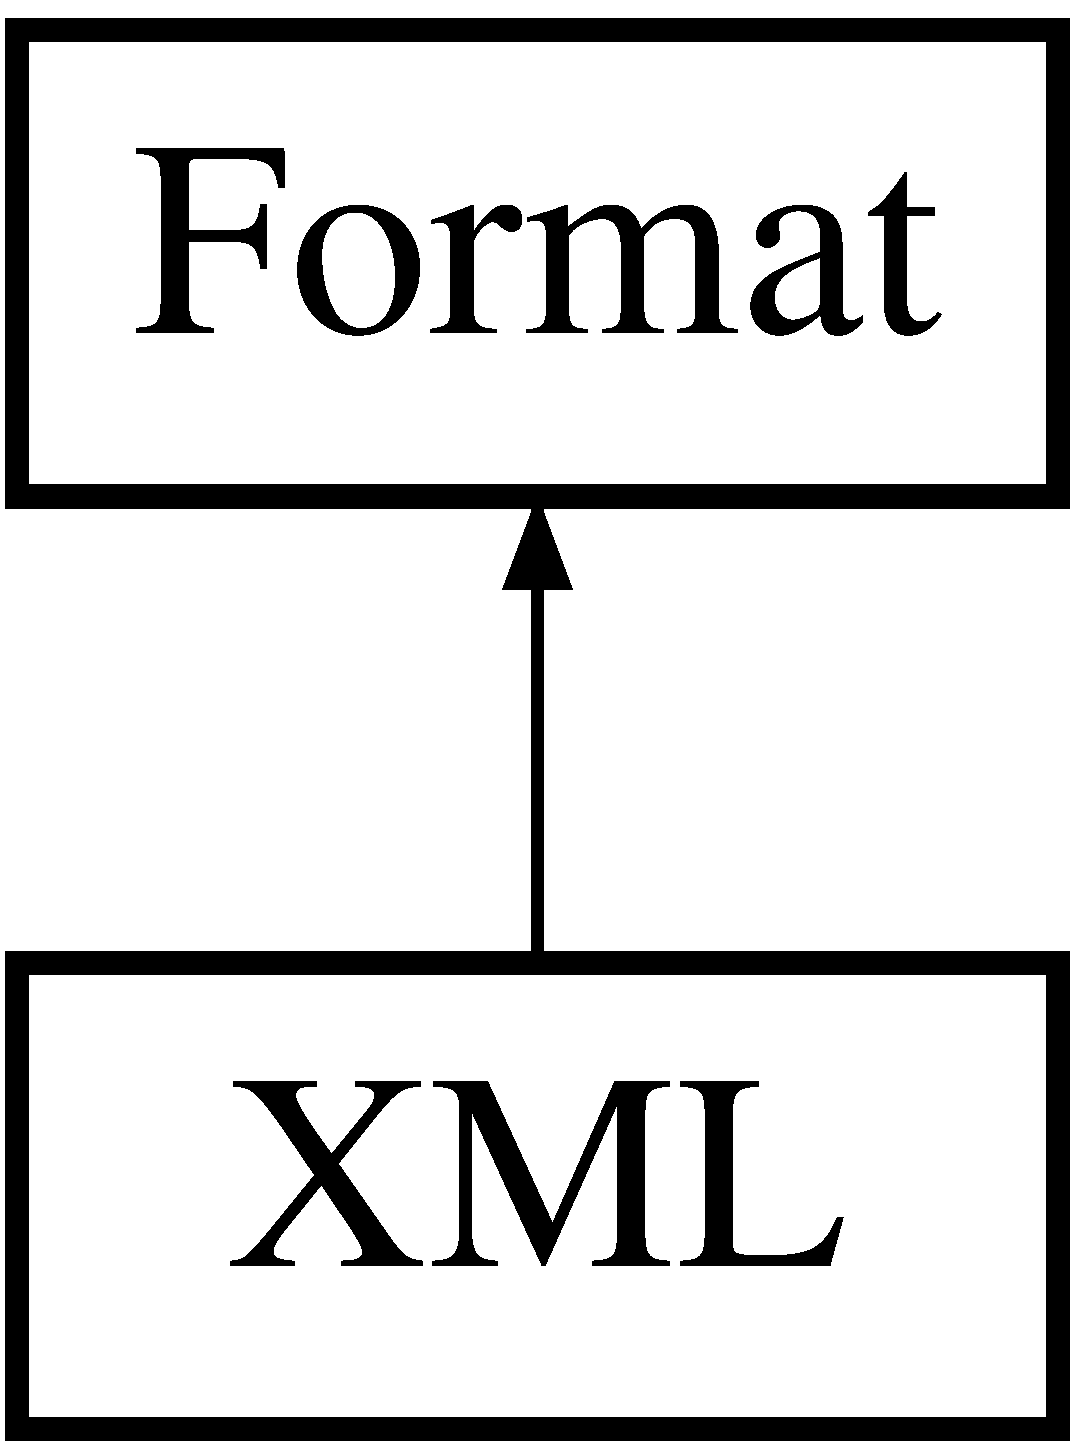
\includegraphics[height=2.000000cm]{class_format}
\end{center}
\end{figure}
\subsection*{Fonctions membres publiques}
\begin{DoxyCompactItemize}
\item 
void \hyperlink{class_format_ad4549bc7712d09a5fd8874e5cffd7c9b}{set\+Pathname} (const Q\+String \&p)
\item 
const Q\+String \& \hyperlink{class_format_a8ef3acfd8d6d5be588e31e6a4a1d789b}{get\+Pathname} ()
\item 
\hypertarget{class_format_a4e2330d6894994551b607e5cbfab42bc}{}virtual void {\bfseries save} () const =0\label{class_format_a4e2330d6894994551b607e5cbfab42bc}

\item 
\hypertarget{class_format_aa571fc1c38b61945d15b999088f43094}{}virtual void {\bfseries load} () const =0\label{class_format_aa571fc1c38b61945d15b999088f43094}

\end{DoxyCompactItemize}
\subsection*{Fonctions membres protégées}
\begin{DoxyCompactItemize}
\item 
\hypertarget{class_format_ae0a81f45095e58dda33592992dcf0289}{}{\bfseries Format} (const Q\+String \&p)\label{class_format_ae0a81f45095e58dda33592992dcf0289}

\item 
\hypertarget{class_format_ab69111c370cfe44f9508e78e5431cc65}{}{\bfseries Format} (const \hyperlink{class_format}{Format} \&)\label{class_format_ab69111c370cfe44f9508e78e5431cc65}

\item 
\hypertarget{class_format_a7a5276a88c488462eea3a508b71f4d9c}{}\hyperlink{class_format}{Format} \& {\bfseries operator=} (const \hyperlink{class_format}{Format} \&)\label{class_format_a7a5276a88c488462eea3a508b71f4d9c}

\end{DoxyCompactItemize}
\subsection*{Attributs protégés}
\begin{DoxyCompactItemize}
\item 
\hypertarget{class_format_a84b62f9b8ac97061cba153dc339b88d4}{}Q\+String {\bfseries pathname}\label{class_format_a84b62f9b8ac97061cba153dc339b88d4}

\end{DoxyCompactItemize}


\subsection{Description détaillée}
\hyperlink{class_format}{Format} est une classe virtuelle pure permettant la mise en place du pattern design Strategy. Les classes fillent qui en héritent peuvent alors être utiliser par le \hyperlink{class_memento}{Memento} afin de réaliser divers types d\textquotesingle{}exportations. 

\subsection{Documentation des fonctions membres}
\hypertarget{class_format_a8ef3acfd8d6d5be588e31e6a4a1d789b}{}\index{Format@{Format}!get\+Pathname@{get\+Pathname}}
\index{get\+Pathname@{get\+Pathname}!Format@{Format}}
\subsubsection[{get\+Pathname}]{\setlength{\rightskip}{0pt plus 5cm}const Q\+String\& Format\+::get\+Pathname (
\begin{DoxyParamCaption}
{}
\end{DoxyParamCaption}
)\hspace{0.3cm}{\ttfamily [inline]}}\label{class_format_a8ef3acfd8d6d5be588e31e6a4a1d789b}
Renvoie le chemin courant du fichier de sauvegarde. \hypertarget{class_format_ad4549bc7712d09a5fd8874e5cffd7c9b}{}\index{Format@{Format}!set\+Pathname@{set\+Pathname}}
\index{set\+Pathname@{set\+Pathname}!Format@{Format}}
\subsubsection[{set\+Pathname}]{\setlength{\rightskip}{0pt plus 5cm}void Format\+::set\+Pathname (
\begin{DoxyParamCaption}
\item[{const Q\+String \&}]{p}
\end{DoxyParamCaption}
)\hspace{0.3cm}{\ttfamily [inline]}}\label{class_format_ad4549bc7712d09a5fd8874e5cffd7c9b}
Modifie le chemin courant du fichier de sauvegarde. 

La documentation de cette classe a été générée à partir du fichier suivant \+:\begin{DoxyCompactItemize}
\item 
import-\/export.\+h\end{DoxyCompactItemize}

\hypertarget{class_t_i_m_e_1_1_horaire}{}\section{Référence de la classe T\+I\+M\+E\+:\+:Horaire}
\label{class_t_i_m_e_1_1_horaire}\index{T\+I\+M\+E\+::\+Horaire@{T\+I\+M\+E\+::\+Horaire}}


Classe permettant de manipuler des horaires L\textquotesingle{}utilisation de cette classe nécessite des dates valides au sens commun du terme. Déclenchement d\textquotesingle{}exception dans le cas contraire.  




{\ttfamily \#include $<$timing.\+h$>$}

\subsection*{Fonctions membres publiques}
\begin{DoxyCompactItemize}
\item 
\hyperlink{class_t_i_m_e_1_1_horaire_ab833c9dc3a4fdbda3894dbbd72643813}{Horaire} (unsigned short int h, unsigned short int m)
\begin{DoxyCompactList}\small\item\em Constructeur à partir de heure et minute. \end{DoxyCompactList}\item 
\hypertarget{class_t_i_m_e_1_1_horaire_ae4dd22490e383b0662fc5788bd42d370}{}void {\bfseries set\+Horaire} (unsigned short int h, unsigned short int m)\label{class_t_i_m_e_1_1_horaire_ae4dd22490e383b0662fc5788bd42d370}

\item 
\hypertarget{class_t_i_m_e_1_1_horaire_af4f27b26ed338d7fa03659107f813cf8}{}void {\bfseries afficher} (std\+::ostream \&f=std\+::cout) const \label{class_t_i_m_e_1_1_horaire_af4f27b26ed338d7fa03659107f813cf8}

\item 
\hypertarget{class_t_i_m_e_1_1_horaire_ace5d2381e38d80e99c6a84158a4044e3}{}unsigned short int {\bfseries get\+Heure} () const \label{class_t_i_m_e_1_1_horaire_ace5d2381e38d80e99c6a84158a4044e3}

\item 
\hypertarget{class_t_i_m_e_1_1_horaire_a5b0e73a520913fd0588407c1507344a8}{}unsigned short int {\bfseries get\+Minute} () const \label{class_t_i_m_e_1_1_horaire_a5b0e73a520913fd0588407c1507344a8}

\item 
\hypertarget{class_t_i_m_e_1_1_horaire_a30ec21c5b5cad95c1c17c02c66d796a6}{}bool {\bfseries operator$<$} (const \hyperlink{class_t_i_m_e_1_1_horaire}{Horaire} \&h) const \label{class_t_i_m_e_1_1_horaire_a30ec21c5b5cad95c1c17c02c66d796a6}

\end{DoxyCompactItemize}


\subsection{Description détaillée}
Classe permettant de manipuler des horaires L\textquotesingle{}utilisation de cette classe nécessite des dates valides au sens commun du terme. Déclenchement d\textquotesingle{}exception dans le cas contraire. 

\subsection{Documentation des constructeurs et destructeur}
\hypertarget{class_t_i_m_e_1_1_horaire_ab833c9dc3a4fdbda3894dbbd72643813}{}\index{T\+I\+M\+E\+::\+Horaire@{T\+I\+M\+E\+::\+Horaire}!Horaire@{Horaire}}
\index{Horaire@{Horaire}!T\+I\+M\+E\+::\+Horaire@{T\+I\+M\+E\+::\+Horaire}}
\subsubsection[{Horaire}]{\setlength{\rightskip}{0pt plus 5cm}T\+I\+M\+E\+::\+Horaire\+::\+Horaire (
\begin{DoxyParamCaption}
\item[{unsigned short int}]{h, }
\item[{unsigned short int}]{m}
\end{DoxyParamCaption}
)\hspace{0.3cm}{\ttfamily [inline]}}\label{class_t_i_m_e_1_1_horaire_ab833c9dc3a4fdbda3894dbbd72643813}


Constructeur à partir de heure et minute. 


\begin{DoxyParams}{Paramètres}
{\em h} & heure avec 0$<$=h$<$=23 \\
\hline
{\em m} & minute avec 0$<$=m$<$=59 \\
\hline
\end{DoxyParams}


La documentation de cette classe a été générée à partir des fichiers suivants \+:\begin{DoxyCompactItemize}
\item 
timing.\+h\item 
timing.\+cpp\end{DoxyCompactItemize}

\hypertarget{class_t_i_m_e_1_1_intervalle}{}\section{Référence de la classe T\+I\+M\+E\+:\+:Intervalle}
\label{class_t_i_m_e_1_1_intervalle}\index{T\+I\+M\+E\+::\+Intervalle@{T\+I\+M\+E\+::\+Intervalle}}


Classe permettant de manipuler des intervalles de dates L\textquotesingle{}utilisation de cette classe nécessite des dates valides au sens commun du terme. Déclenchement d\textquotesingle{}exception dans le cas contraire.  




{\ttfamily \#include $<$timing.\+h$>$}

\subsection*{Fonctions membres publiques}
\begin{DoxyCompactItemize}
\item 
\hyperlink{class_t_i_m_e_1_1_intervalle_a98b63f9c55a777090ec224d61ab26427}{Intervalle} (const \hyperlink{class_t_i_m_e_1_1_date}{Date} \&d, const \hyperlink{class_t_i_m_e_1_1_date}{Date} \&f)
\begin{DoxyCompactList}\small\item\em Constructeur à partir de deux dates. \end{DoxyCompactList}\item 
\hypertarget{class_t_i_m_e_1_1_intervalle_a729d464967de6618da00b772357dc923}{}void {\bfseries afficher} (std\+::ostream \&f=std\+::cout) const \label{class_t_i_m_e_1_1_intervalle_a729d464967de6618da00b772357dc923}

\item 
\hypertarget{class_t_i_m_e_1_1_intervalle_a8a9980c16e051af5e08135815cc3d074}{}\hyperlink{class_t_i_m_e_1_1_date}{Date} {\bfseries get\+Debut} () const \label{class_t_i_m_e_1_1_intervalle_a8a9980c16e051af5e08135815cc3d074}

\item 
\hypertarget{class_t_i_m_e_1_1_intervalle_a20a035fb9d9720ef94e62e1ef45845c3}{}\hyperlink{class_t_i_m_e_1_1_date}{Date} {\bfseries get\+Fin} () const \label{class_t_i_m_e_1_1_intervalle_a20a035fb9d9720ef94e62e1ef45845c3}

\item 
\hypertarget{class_t_i_m_e_1_1_intervalle_adec63857259b690f79de8d16b0ca0c4d}{}int {\bfseries get\+Duree} () const \label{class_t_i_m_e_1_1_intervalle_adec63857259b690f79de8d16b0ca0c4d}

\item 
\hypertarget{class_t_i_m_e_1_1_intervalle_a8f7dca71eb9d8648fa30225360df4fda}{}bool {\bfseries operator\&\&} (const \hyperlink{class_t_i_m_e_1_1_intervalle}{Intervalle} \&v) const \label{class_t_i_m_e_1_1_intervalle_a8f7dca71eb9d8648fa30225360df4fda}

\item 
\hypertarget{class_t_i_m_e_1_1_intervalle_a9dfead5501b190507a2ffa5c29450ffe}{}\hyperlink{class_t_i_m_e_1_1_intervalle}{Intervalle} {\bfseries operator+} (const \hyperlink{class_t_i_m_e_1_1_intervalle}{Intervalle} \&i) const \label{class_t_i_m_e_1_1_intervalle_a9dfead5501b190507a2ffa5c29450ffe}

\end{DoxyCompactItemize}


\subsection{Description détaillée}
Classe permettant de manipuler des intervalles de dates L\textquotesingle{}utilisation de cette classe nécessite des dates valides au sens commun du terme. Déclenchement d\textquotesingle{}exception dans le cas contraire. 

\subsection{Documentation des constructeurs et destructeur}
\hypertarget{class_t_i_m_e_1_1_intervalle_a98b63f9c55a777090ec224d61ab26427}{}\index{T\+I\+M\+E\+::\+Intervalle@{T\+I\+M\+E\+::\+Intervalle}!Intervalle@{Intervalle}}
\index{Intervalle@{Intervalle}!T\+I\+M\+E\+::\+Intervalle@{T\+I\+M\+E\+::\+Intervalle}}
\subsubsection[{Intervalle}]{\setlength{\rightskip}{0pt plus 5cm}Intervalle\+::\+Intervalle (
\begin{DoxyParamCaption}
\item[{const {\bf Date} \&}]{d, }
\item[{const {\bf Date} \&}]{f}
\end{DoxyParamCaption}
)}\label{class_t_i_m_e_1_1_intervalle_a98b63f9c55a777090ec224d61ab26427}


Constructeur à partir de deux dates. 


\begin{DoxyParams}{Paramètres}
{\em d} & date de début de l\textquotesingle{}intervalle \\
\hline
{\em f} & date de fin de l\textquotesingle{}intervalle. On doit avoir d$<$=f \\
\hline
\end{DoxyParams}


La documentation de cette classe a été générée à partir des fichiers suivants \+:\begin{DoxyCompactItemize}
\item 
timing.\+h\item 
timing.\+cpp\end{DoxyCompactItemize}

\hypertarget{class_tache_composite_1_1iterator}{}\section{Référence de la classe Tache\+Composite\+:\+:iterator}
\label{class_tache_composite_1_1iterator}\index{Tache\+Composite\+::iterator@{Tache\+Composite\+::iterator}}
Graphe d\textquotesingle{}héritage de Tache\+Composite\+:\+:iterator\+:\begin{figure}[H]
\begin{center}
\leavevmode
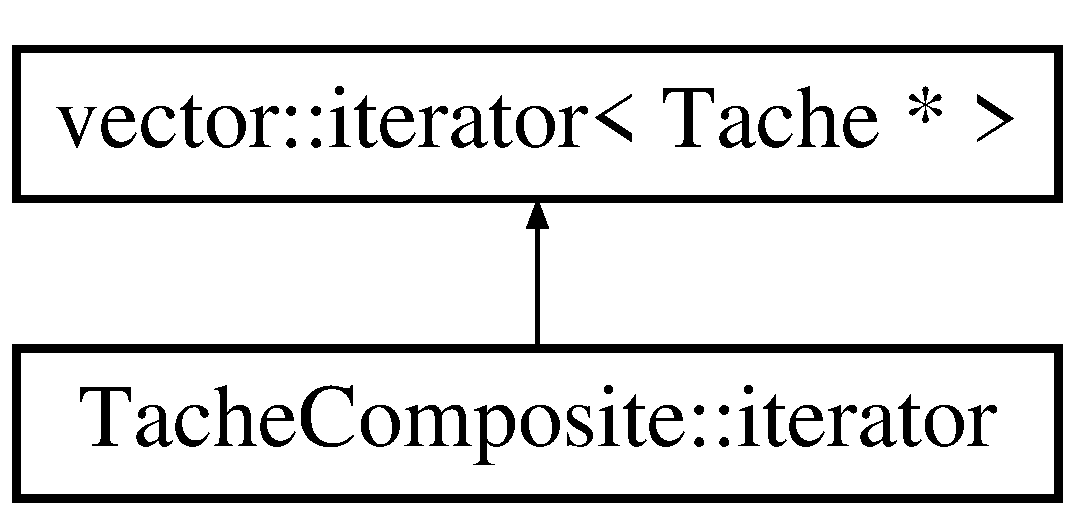
\includegraphics[height=2.000000cm]{class_tache_composite_1_1iterator}
\end{center}
\end{figure}
\subsection*{Fonctions membres publiques}
\begin{DoxyCompactItemize}
\item 
\hypertarget{class_tache_composite_1_1iterator_af1c995574219e4dd0342bed04b97ebbc}{}{\bfseries iterator} (vector$<$ \hyperlink{class_tache}{Tache} $\ast$ $>$\+::\hyperlink{class_tache_composite_1_1iterator}{iterator} it)\label{class_tache_composite_1_1iterator_af1c995574219e4dd0342bed04b97ebbc}

\end{DoxyCompactItemize}


La documentation de cette classe a été générée à partir du fichier suivant \+:\begin{DoxyCompactItemize}
\item 
evenement.\+h\end{DoxyCompactItemize}

\hypertarget{class_projet_1_1iterator}{}\section{Référence de la classe Projet\+:\+:iterator}
\label{class_projet_1_1iterator}\index{Projet\+::iterator@{Projet\+::iterator}}
Graphe d\textquotesingle{}héritage de Projet\+:\+:iterator\+:\begin{figure}[H]
\begin{center}
\leavevmode
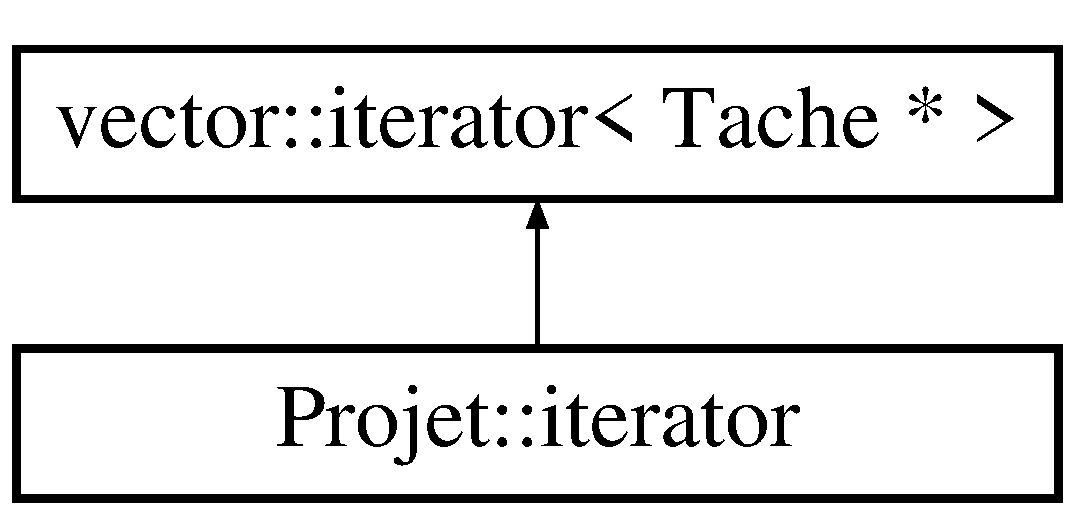
\includegraphics[height=2.000000cm]{class_projet_1_1iterator}
\end{center}
\end{figure}
\subsection*{Fonctions membres publiques}
\begin{DoxyCompactItemize}
\item 
\hypertarget{class_projet_1_1iterator_a1969381a91b0dc84a8bfd11e0c98c023}{}{\bfseries iterator} (vector$<$ \hyperlink{class_tache}{Tache} $\ast$ $>$\+::\hyperlink{class_projet_1_1iterator}{iterator} it)\label{class_projet_1_1iterator_a1969381a91b0dc84a8bfd11e0c98c023}

\end{DoxyCompactItemize}


La documentation de cette classe a été générée à partir du fichier suivant \+:\begin{DoxyCompactItemize}
\item 
evenement.\+h\end{DoxyCompactItemize}

\hypertarget{class_manager_1_1iterator}{}\section{Référence de la classe Manager$<$ T, U $>$\+:\+:iterator}
\label{class_manager_1_1iterator}\index{Manager$<$ T, U $>$\+::iterator@{Manager$<$ T, U $>$\+::iterator}}
Graphe d\textquotesingle{}héritage de Manager$<$ T, U $>$\+:\+:iterator\+:\begin{figure}[H]
\begin{center}
\leavevmode
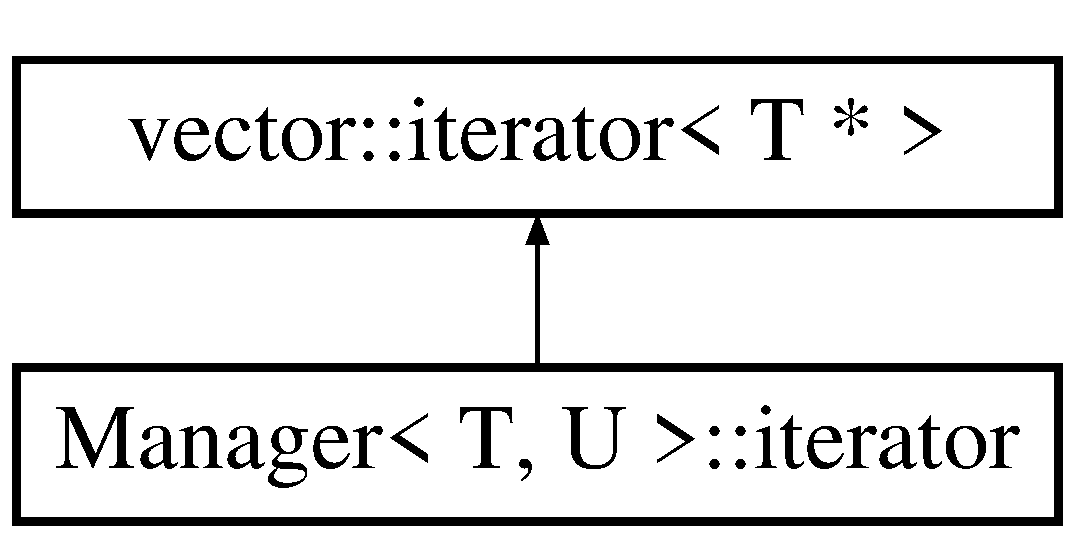
\includegraphics[height=2.000000cm]{class_manager_1_1iterator}
\end{center}
\end{figure}
\subsection*{Fonctions membres publiques}
\begin{DoxyCompactItemize}
\item 
\hypertarget{class_manager_1_1iterator_a9d451fc2bd2298ecddeabd4cc817e8ec}{}{\bfseries iterator} (typename vector$<$ T $\ast$ $>$\+::\hyperlink{class_manager_1_1iterator}{iterator} it)\label{class_manager_1_1iterator_a9d451fc2bd2298ecddeabd4cc817e8ec}

\end{DoxyCompactItemize}


La documentation de cette classe a été générée à partir du fichier suivant \+:\begin{DoxyCompactItemize}
\item 
manager.\+h\end{DoxyCompactItemize}

\hypertarget{class_main_window}{}\section{Référence de la classe Main\+Window}
\label{class_main_window}\index{Main\+Window@{Main\+Window}}


Fenêtre Principale du calendrier.  




{\ttfamily \#include $<$mainwindow.\+h$>$}

Graphe d\textquotesingle{}héritage de Main\+Window\+:\begin{figure}[H]
\begin{center}
\leavevmode
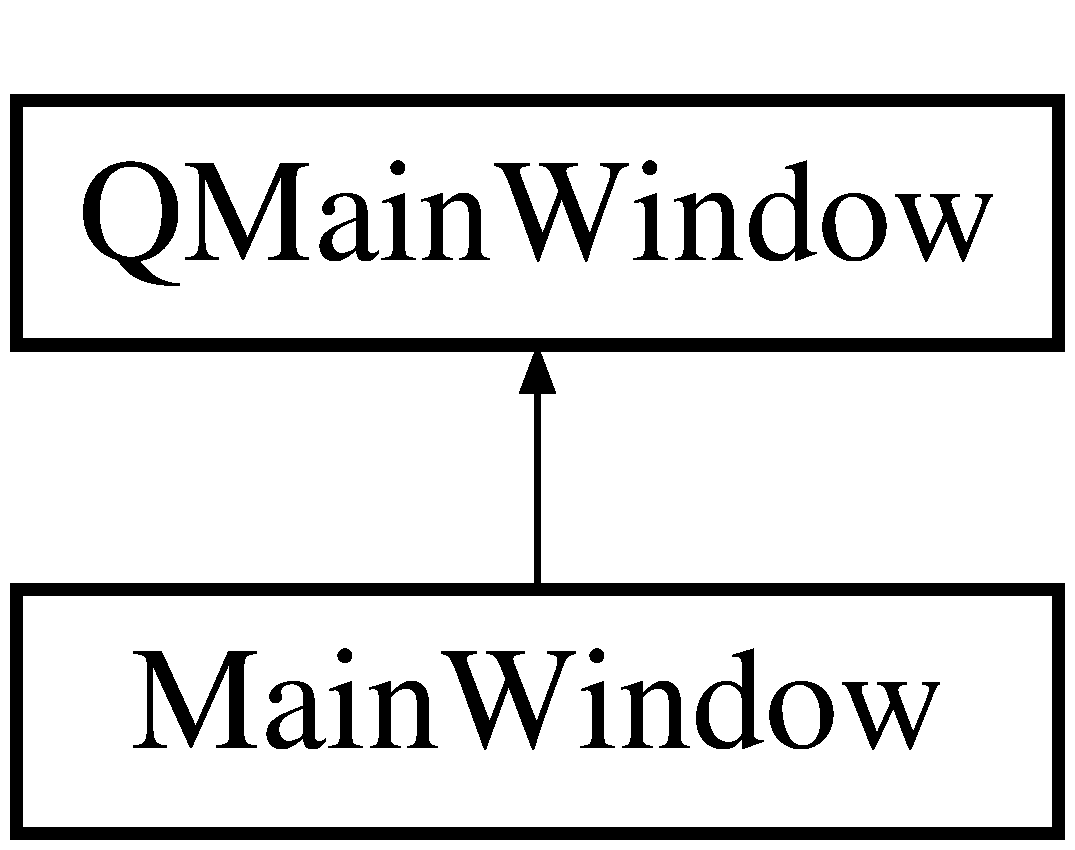
\includegraphics[height=2.000000cm]{class_main_window}
\end{center}
\end{figure}
\subsection*{Fonctions membres publiques}
\begin{DoxyCompactItemize}
\item 
\hypertarget{class_main_window_a8b244be8b7b7db1b08de2a2acb9409db}{}{\bfseries Main\+Window} (Q\+Widget $\ast$parent=0)\label{class_main_window_a8b244be8b7b7db1b08de2a2acb9409db}

\item 
\hypertarget{class_main_window_ae29bd136b47fdb473f80ce007e079b0c}{}void {\bfseries refresh\+\_\+calendar} (const Q\+Date \&date)\label{class_main_window_ae29bd136b47fdb473f80ce007e079b0c}

\item 
\hypertarget{class_main_window_afbd226d0f42df6f1436114bd96ea4d7d}{}void {\bfseries refresh\+\_\+calendar} ()\label{class_main_window_afbd226d0f42df6f1436114bd96ea4d7d}

\item 
\hypertarget{class_main_window_aa9c7f49a5902ddc911a117d547781aa7}{}const Q\+Date \& {\bfseries get\+Current\+Date} () const \label{class_main_window_aa9c7f49a5902ddc911a117d547781aa7}

\end{DoxyCompactItemize}


\subsection{Description détaillée}
Fenêtre Principale du calendrier. 

La documentation de cette classe a été générée à partir des fichiers suivants \+:\begin{DoxyCompactItemize}
\item 
G\+U\+I/mainwindow.\+h\item 
G\+U\+I/mainwindow.\+cpp\end{DoxyCompactItemize}

\hypertarget{class_manager}{}\section{Référence du modèle de la classe Manager$<$ T, U $>$}
\label{class_manager}\index{Manager$<$ T, U $>$@{Manager$<$ T, U $>$}}


{\ttfamily \#include $<$manager.\+h$>$}

\subsection*{Classes}
\begin{DoxyCompactItemize}
\item 
class \hyperlink{class_manager_1_1const__iterator}{const\+\_\+iterator}
\item 
class \hyperlink{class_manager_1_1iterator}{iterator}
\end{DoxyCompactItemize}
\subsection*{Fonctions membres publiques}
\begin{DoxyCompactItemize}
\item 
unsigned int \hyperlink{class_manager_adf66a1a70fdd9dc6cdaa13b0c5b4d834}{get\+Size} () const 
\item 
T $\ast$ \hyperlink{class_manager_a1a4856f30411e79051523887d0f251b8}{get\+Item} (const Q\+String \&id)
\item 
bool \hyperlink{class_manager_a8edf2ecc36ad33ba354ccabff3210d23}{is\+Id\+Free} (const Q\+String \&id)
\item 
void \hyperlink{class_manager_ac9136f779f6075c6be1437db35b31468}{delete\+Item} (T \&t)
\item 
void \hyperlink{class_manager_a6e003fb43ed160833e3094d1a59874e3}{delete\+Item} (const Q\+String \&id)
\item 
virtual void \hyperlink{class_manager_a151e9d0a033a7fa21c2d84221f22b01f}{delete\+Item} (\hyperlink{class_manager_1_1iterator}{iterator} it)
\item 
\hyperlink{class_manager_1_1iterator}{iterator} \hyperlink{class_manager_ad2d2c9ac1c765c3db47cb49f926e4494}{begin} ()
\item 
\hyperlink{class_manager_1_1iterator}{iterator} \hyperlink{class_manager_ab438bec0cd793093bee6c8f12c05b32a}{end} ()
\item 
\hyperlink{class_manager_1_1const__iterator}{const\+\_\+iterator} \hyperlink{class_manager_ad53e3636df68daf3cc47ce59da98db6d}{begin} () const 
\item 
\hyperlink{class_manager_1_1const__iterator}{const\+\_\+iterator} \hyperlink{class_manager_a15006050d43cbaef467051ff53faa8bd}{end} () const 
\end{DoxyCompactItemize}
\subsection*{Fonctions membres publiques statiques}
\begin{DoxyCompactItemize}
\item 
static U \& \hyperlink{class_manager_a8372e4f1e14f3605a57d839b152325ed}{get\+Instance} ()
\item 
static void \hyperlink{class_manager_ada15725fe33d625e2c06dcbe2c5edc4e}{free\+Instance} ()
\end{DoxyCompactItemize}
\subsection*{Fonctions membres protégées}
\begin{DoxyCompactItemize}
\item 
\hypertarget{class_manager_ada69ae9ca42784e98fb81b1fdbcfc6a6}{}void {\bfseries add\+Item} (T \&t)\label{class_manager_ada69ae9ca42784e98fb81b1fdbcfc6a6}

\end{DoxyCompactItemize}
\subsection*{Attributs protégés}
\begin{DoxyCompactItemize}
\item 
\hypertarget{class_manager_abbf456c6a3b97e3a4106316545cbfe69}{}vector$<$ T $\ast$ $>$ {\bfseries tab}\label{class_manager_abbf456c6a3b97e3a4106316545cbfe69}

\end{DoxyCompactItemize}
\subsection*{Attributs protégés statiques}
\begin{DoxyCompactItemize}
\item 
\hypertarget{class_manager_a2b5df0a89665c24f3a01f36ac6f725aa}{}static Handler {\bfseries handler}\label{class_manager_a2b5df0a89665c24f3a01f36ac6f725aa}

\end{DoxyCompactItemize}


\subsection{Description détaillée}
\subsubsection*{template$<$class T, class U$>$class Manager$<$ T, U $>$}

La classe \hyperlink{class_manager}{Manager} est un singleton conteneur d\textquotesingle{}items. Elle gère le cycle de vie de ses items, de la création à la destruction en passant par la modification. Une façade d\textquotesingle{}iterator a été mise en place pour empêcher l\textquotesingle{}accès direct au vecteur privé contenant les items. Celle-\/ci est virtuelle pure, ainsi seules ses classes filles peuvent être instanciées\+:
\begin{DoxyItemize}
\item \hyperlink{class_projet_manager}{Projet\+Manager}
\item \hyperlink{class_activite_manager}{Activite\+Manager}
\item \hyperlink{class_tache_manager}{Tache\+Manager}
\item \hyperlink{class_programmation_manager}{Programmation\+Manager}
\item \hyperlink{class_precedence_manager}{Precedence\+Manager}
\end{DoxyItemize}

Un Handler a également été mis en place permettant la désallocation automatique du \hyperlink{class_manager}{Manager} à la fin du processus. 

\subsection{Documentation des fonctions membres}
\hypertarget{class_manager_ad2d2c9ac1c765c3db47cb49f926e4494}{}\index{Manager@{Manager}!begin@{begin}}
\index{begin@{begin}!Manager@{Manager}}
\subsubsection[{begin}]{\setlength{\rightskip}{0pt plus 5cm}template$<$class T, class U$>$ {\bf iterator} {\bf Manager}$<$ T, U $>$\+::begin (
\begin{DoxyParamCaption}
{}
\end{DoxyParamCaption}
)\hspace{0.3cm}{\ttfamily [inline]}}\label{class_manager_ad2d2c9ac1c765c3db47cb49f926e4494}
Renvoie un iterator sur le premier item du vecteur. \hypertarget{class_manager_ad53e3636df68daf3cc47ce59da98db6d}{}\index{Manager@{Manager}!begin@{begin}}
\index{begin@{begin}!Manager@{Manager}}
\subsubsection[{begin}]{\setlength{\rightskip}{0pt plus 5cm}template$<$class T, class U$>$ {\bf const\+\_\+iterator} {\bf Manager}$<$ T, U $>$\+::begin (
\begin{DoxyParamCaption}
{}
\end{DoxyParamCaption}
) const\hspace{0.3cm}{\ttfamily [inline]}}\label{class_manager_ad53e3636df68daf3cc47ce59da98db6d}
Renvoie un \hyperlink{class_manager_1_1const__iterator}{const\+\_\+iterator} sur le premier item du vecteur. \hypertarget{class_manager_ac9136f779f6075c6be1437db35b31468}{}\index{Manager@{Manager}!delete\+Item@{delete\+Item}}
\index{delete\+Item@{delete\+Item}!Manager@{Manager}}
\subsubsection[{delete\+Item}]{\setlength{\rightskip}{0pt plus 5cm}template$<$class T, class U $>$ void {\bf Manager}$<$ T, U $>$\+::delete\+Item (
\begin{DoxyParamCaption}
\item[{T \&}]{t}
\end{DoxyParamCaption}
)}\label{class_manager_ac9136f779f6075c6be1437db35b31468}
Supprime l\textquotesingle{}item dont la référence a été passée en paramètre. \hypertarget{class_manager_a6e003fb43ed160833e3094d1a59874e3}{}\index{Manager@{Manager}!delete\+Item@{delete\+Item}}
\index{delete\+Item@{delete\+Item}!Manager@{Manager}}
\subsubsection[{delete\+Item}]{\setlength{\rightskip}{0pt plus 5cm}template$<$class T, class U $>$ void {\bf Manager}$<$ T, U $>$\+::delete\+Item (
\begin{DoxyParamCaption}
\item[{const Q\+String \&}]{id}
\end{DoxyParamCaption}
)}\label{class_manager_a6e003fb43ed160833e3094d1a59874e3}
Supprime l\textquotesingle{}item dont l\textquotesingle{}identificateur a été passé en paramètre. \hypertarget{class_manager_a151e9d0a033a7fa21c2d84221f22b01f}{}\index{Manager@{Manager}!delete\+Item@{delete\+Item}}
\index{delete\+Item@{delete\+Item}!Manager@{Manager}}
\subsubsection[{delete\+Item}]{\setlength{\rightskip}{0pt plus 5cm}template$<$class T, class U $>$ void {\bf Manager}$<$ T, U $>$\+::delete\+Item (
\begin{DoxyParamCaption}
\item[{{\bf iterator}}]{it}
\end{DoxyParamCaption}
)\hspace{0.3cm}{\ttfamily [inline]}, {\ttfamily [virtual]}}\label{class_manager_a151e9d0a033a7fa21c2d84221f22b01f}
Supprime l\textquotesingle{}item pointé par l\textquotesingle{}iterator passé en paramètre. \hypertarget{class_manager_ab438bec0cd793093bee6c8f12c05b32a}{}\index{Manager@{Manager}!end@{end}}
\index{end@{end}!Manager@{Manager}}
\subsubsection[{end}]{\setlength{\rightskip}{0pt plus 5cm}template$<$class T, class U$>$ {\bf iterator} {\bf Manager}$<$ T, U $>$\+::end (
\begin{DoxyParamCaption}
{}
\end{DoxyParamCaption}
)\hspace{0.3cm}{\ttfamily [inline]}}\label{class_manager_ab438bec0cd793093bee6c8f12c05b32a}
Renvoie un iterator sur la fin du vecteur. \hypertarget{class_manager_a15006050d43cbaef467051ff53faa8bd}{}\index{Manager@{Manager}!end@{end}}
\index{end@{end}!Manager@{Manager}}
\subsubsection[{end}]{\setlength{\rightskip}{0pt plus 5cm}template$<$class T, class U$>$ {\bf const\+\_\+iterator} {\bf Manager}$<$ T, U $>$\+::end (
\begin{DoxyParamCaption}
{}
\end{DoxyParamCaption}
) const\hspace{0.3cm}{\ttfamily [inline]}}\label{class_manager_a15006050d43cbaef467051ff53faa8bd}
Renvoie un \hyperlink{class_manager_1_1const__iterator}{const\+\_\+iterator} sur la fin du vecteur. \hypertarget{class_manager_ada15725fe33d625e2c06dcbe2c5edc4e}{}\index{Manager@{Manager}!free\+Instance@{free\+Instance}}
\index{free\+Instance@{free\+Instance}!Manager@{Manager}}
\subsubsection[{free\+Instance}]{\setlength{\rightskip}{0pt plus 5cm}template$<$class T , class U $>$ void {\bf Manager}$<$ T, U $>$\+::free\+Instance (
\begin{DoxyParamCaption}
{}
\end{DoxyParamCaption}
)\hspace{0.3cm}{\ttfamily [static]}}\label{class_manager_ada15725fe33d625e2c06dcbe2c5edc4e}
Libère l\textquotesingle{}instance du \hyperlink{class_manager}{Manager}, et entraine sa désallocation mémoire. \hypertarget{class_manager_a8372e4f1e14f3605a57d839b152325ed}{}\index{Manager@{Manager}!get\+Instance@{get\+Instance}}
\index{get\+Instance@{get\+Instance}!Manager@{Manager}}
\subsubsection[{get\+Instance}]{\setlength{\rightskip}{0pt plus 5cm}template$<$class T , class U $>$ U \& {\bf Manager}$<$ T, U $>$\+::get\+Instance (
\begin{DoxyParamCaption}
{}
\end{DoxyParamCaption}
)\hspace{0.3cm}{\ttfamily [static]}}\label{class_manager_a8372e4f1e14f3605a57d839b152325ed}
Renvoie une référence sur l\textquotesingle{}instance du \hyperlink{class_manager}{Manager}. Si ce dernier n\textquotesingle{}est pas créé lors de l\textquotesingle{}appel, la méthode instancie le \hyperlink{class_manager}{Manager} et renvoie sa référence. \hypertarget{class_manager_a1a4856f30411e79051523887d0f251b8}{}\index{Manager@{Manager}!get\+Item@{get\+Item}}
\index{get\+Item@{get\+Item}!Manager@{Manager}}
\subsubsection[{get\+Item}]{\setlength{\rightskip}{0pt plus 5cm}template$<$class T , class U $>$ T $\ast$ {\bf Manager}$<$ T, U $>$\+::get\+Item (
\begin{DoxyParamCaption}
\item[{const Q\+String \&}]{id}
\end{DoxyParamCaption}
)}\label{class_manager_a1a4856f30411e79051523887d0f251b8}
Renvoie un pointeur sur l\textquotesingle{}item dont l\textquotesingle{}identificateur a été passé en paramètre Si ce dernier n\textquotesingle{}existe pas, nullptr est retourné. \hypertarget{class_manager_adf66a1a70fdd9dc6cdaa13b0c5b4d834}{}\index{Manager@{Manager}!get\+Size@{get\+Size}}
\index{get\+Size@{get\+Size}!Manager@{Manager}}
\subsubsection[{get\+Size}]{\setlength{\rightskip}{0pt plus 5cm}template$<$class T, class U$>$ unsigned int {\bf Manager}$<$ T, U $>$\+::get\+Size (
\begin{DoxyParamCaption}
{}
\end{DoxyParamCaption}
) const\hspace{0.3cm}{\ttfamily [inline]}}\label{class_manager_adf66a1a70fdd9dc6cdaa13b0c5b4d834}
Retourne le nombre d\textquotesingle{}items contenus dans le vecteur. \hypertarget{class_manager_a8edf2ecc36ad33ba354ccabff3210d23}{}\index{Manager@{Manager}!is\+Id\+Free@{is\+Id\+Free}}
\index{is\+Id\+Free@{is\+Id\+Free}!Manager@{Manager}}
\subsubsection[{is\+Id\+Free}]{\setlength{\rightskip}{0pt plus 5cm}template$<$class T , class U $>$ bool {\bf Manager}$<$ T, U $>$\+::is\+Id\+Free (
\begin{DoxyParamCaption}
\item[{const Q\+String \&}]{id}
\end{DoxyParamCaption}
)}\label{class_manager_a8edf2ecc36ad33ba354ccabff3210d23}
Vérifie si l\textquotesingle{}identificateur passé en paramètre est déjà existant (il ne peut y avoir de doublon). Renvoie false si déjà existant, sinon retourne vrai. 

La documentation de cette classe a été générée à partir des fichiers suivants \+:\begin{DoxyCompactItemize}
\item 
evenement.\+h\item 
manager.\+h\end{DoxyCompactItemize}

\hypertarget{class_memento}{}\section{Référence de la classe Memento}
\label{class_memento}\index{Memento@{Memento}}


La classe \hyperlink{class_memento}{Memento} est un singleton memento permettant de charger et de sauvegarder l\textquotesingle{}ensemble des informations du calendrier. Elle les exporter selon une stratégie particulière, correspondant au format d\textquotesingle{}exportation. Cette stratégie peut être changée à tout moment par le biais de la méthode set\+Strategie. De plus, elle ne peut être instanciée directement mais peut être récupérer par le biais d\textquotesingle{}une référence ou d\textquotesingle{}un pointeur grâce à la méthode \hyperlink{class_memento_a0d8167075a7e5f8890d8cbe1bd3d1273}{get\+Instance()}. Un Handler a été mis en place afin désalloué automatiquement l\textquotesingle{}instance en fin de processus.  




{\ttfamily \#include $<$import-\/export.\+h$>$}

\subsection*{Fonctions membres publiques}
\begin{DoxyCompactItemize}
\item 
void \hyperlink{class_memento_a2ab0539c90bdafdce79776841f3f835b}{set\+Strategie} (\hyperlink{class_format}{Format} $\ast$strat)
\item 
void \hyperlink{class_memento_a36b2b96d212c9fe1338e80ae41912fa3}{save} () const 
\item 
void \hyperlink{class_memento_a05119b7214605862ef8e48d0d6bb2713}{load} () const 
\end{DoxyCompactItemize}
\subsection*{Fonctions membres publiques statiques}
\begin{DoxyCompactItemize}
\item 
static void \hyperlink{class_memento_a8e97e83e767bd9cb13c6ddcf16125553}{free\+Instance} ()
\item 
static \hyperlink{class_memento}{Memento} \& \hyperlink{class_memento_a0d8167075a7e5f8890d8cbe1bd3d1273}{get\+Instance} (\hyperlink{class_format}{Format} \&strategie=X\+M\+L\+::get\+Instance())
\end{DoxyCompactItemize}


\subsection{Description détaillée}
La classe \hyperlink{class_memento}{Memento} est un singleton memento permettant de charger et de sauvegarder l\textquotesingle{}ensemble des informations du calendrier. Elle les exporter selon une stratégie particulière, correspondant au format d\textquotesingle{}exportation. Cette stratégie peut être changée à tout moment par le biais de la méthode set\+Strategie. De plus, elle ne peut être instanciée directement mais peut être récupérer par le biais d\textquotesingle{}une référence ou d\textquotesingle{}un pointeur grâce à la méthode \hyperlink{class_memento_a0d8167075a7e5f8890d8cbe1bd3d1273}{get\+Instance()}. Un Handler a été mis en place afin désalloué automatiquement l\textquotesingle{}instance en fin de processus. 

\subsection{Documentation des fonctions membres}
\hypertarget{class_memento_a8e97e83e767bd9cb13c6ddcf16125553}{}\index{Memento@{Memento}!free\+Instance@{free\+Instance}}
\index{free\+Instance@{free\+Instance}!Memento@{Memento}}
\subsubsection[{free\+Instance}]{\setlength{\rightskip}{0pt plus 5cm}void Memento\+::free\+Instance (
\begin{DoxyParamCaption}
{}
\end{DoxyParamCaption}
)\hspace{0.3cm}{\ttfamily [static]}}\label{class_memento_a8e97e83e767bd9cb13c6ddcf16125553}
Libère l\textquotesingle{}instance du \hyperlink{class_memento}{Memento} et entraine sa désallocation mémoire. \hypertarget{class_memento_a0d8167075a7e5f8890d8cbe1bd3d1273}{}\index{Memento@{Memento}!get\+Instance@{get\+Instance}}
\index{get\+Instance@{get\+Instance}!Memento@{Memento}}
\subsubsection[{get\+Instance}]{\setlength{\rightskip}{0pt plus 5cm}{\bf Memento} \& Memento\+::get\+Instance (
\begin{DoxyParamCaption}
\item[{{\bf Format} \&}]{strategie = {\ttfamily XML\+:\+:getInstance()}}
\end{DoxyParamCaption}
)\hspace{0.3cm}{\ttfamily [static]}}\label{class_memento_a0d8167075a7e5f8890d8cbe1bd3d1273}
Instancie un objet de la classe \hyperlink{class_memento}{Memento} si aucune instanciation n\textquotesingle{}a été faite au préalable, et retourne sa référence. 
\begin{DoxyParams}{Paramètres}
{\em strategie} & Renvoie une reference sur l\textquotesingle{}instance de \hyperlink{class_memento}{Memento}. \\
\hline
\end{DoxyParams}
\hypertarget{class_memento_a05119b7214605862ef8e48d0d6bb2713}{}\index{Memento@{Memento}!load@{load}}
\index{load@{load}!Memento@{Memento}}
\subsubsection[{load}]{\setlength{\rightskip}{0pt plus 5cm}void Memento\+::load (
\begin{DoxyParamCaption}
{}
\end{DoxyParamCaption}
) const\hspace{0.3cm}{\ttfamily [inline]}}\label{class_memento_a05119b7214605862ef8e48d0d6bb2713}
Charge toutes les informations du calendrier à l\textquotesingle{}aide de la méthode \hyperlink{class_memento_a05119b7214605862ef8e48d0d6bb2713}{load()} de la stratégie actuelle. \hypertarget{class_memento_a36b2b96d212c9fe1338e80ae41912fa3}{}\index{Memento@{Memento}!save@{save}}
\index{save@{save}!Memento@{Memento}}
\subsubsection[{save}]{\setlength{\rightskip}{0pt plus 5cm}void Memento\+::save (
\begin{DoxyParamCaption}
{}
\end{DoxyParamCaption}
) const\hspace{0.3cm}{\ttfamily [inline]}}\label{class_memento_a36b2b96d212c9fe1338e80ae41912fa3}
Sauve toutes les informations du calendrier à l\textquotesingle{}aide de la méthode de la stratégie actuelle. \hypertarget{class_memento_a2ab0539c90bdafdce79776841f3f835b}{}\index{Memento@{Memento}!set\+Strategie@{set\+Strategie}}
\index{set\+Strategie@{set\+Strategie}!Memento@{Memento}}
\subsubsection[{set\+Strategie}]{\setlength{\rightskip}{0pt plus 5cm}void Memento\+::set\+Strategie (
\begin{DoxyParamCaption}
\item[{{\bf Format} $\ast$}]{strat}
\end{DoxyParamCaption}
)\hspace{0.3cm}{\ttfamily [inline]}}\label{class_memento_a2ab0539c90bdafdce79776841f3f835b}
Modifie la stratégie avec celle passée en paramètre 

La documentation de cette classe a été générée à partir des fichiers suivants \+:\begin{DoxyCompactItemize}
\item 
import-\/export.\+h\item 
import-\/export.\+cpp\end{DoxyCompactItemize}

\hypertarget{classouvrirsave}{}\section{Référence de la classe ouvrirsave}
\label{classouvrirsave}\index{ouvrirsave@{ouvrirsave}}


Fenêtre du choix de fichier de sauvegarde.  




{\ttfamily \#include $<$ouvrirsave.\+h$>$}

Graphe d\textquotesingle{}héritage de ouvrirsave\+:\begin{figure}[H]
\begin{center}
\leavevmode
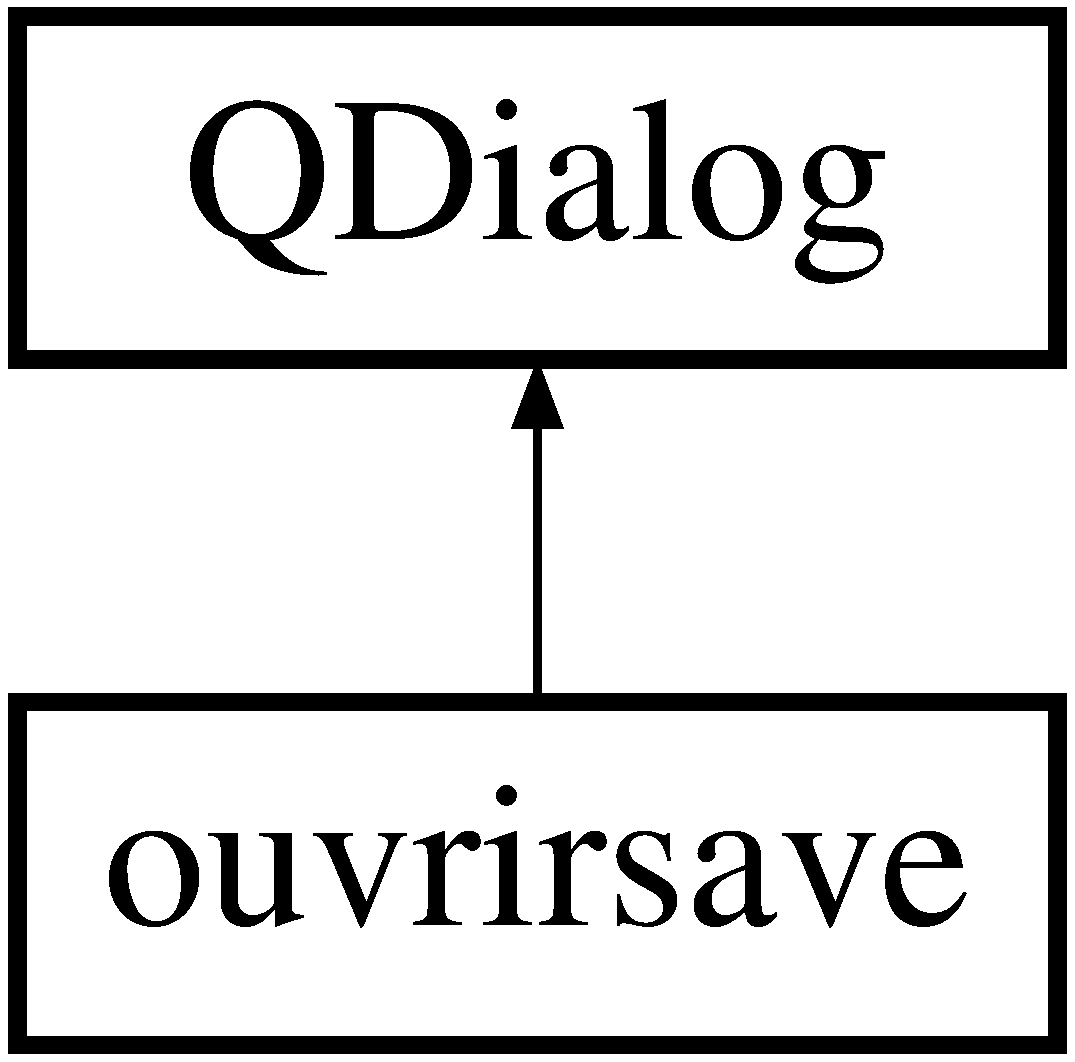
\includegraphics[height=2.000000cm]{classouvrirsave}
\end{center}
\end{figure}
\subsection*{Fonctions membres publiques}
\begin{DoxyCompactItemize}
\item 
\hypertarget{classouvrirsave_a3dd0e7eeb7cd7bebae55f167ee85eb29}{}{\bfseries ouvrirsave} (Q\+Widget $\ast$parent=0)\label{classouvrirsave_a3dd0e7eeb7cd7bebae55f167ee85eb29}

\end{DoxyCompactItemize}


\subsection{Description détaillée}
Fenêtre du choix de fichier de sauvegarde. 

La documentation de cette classe a été générée à partir des fichiers suivants \+:\begin{DoxyCompactItemize}
\item 
G\+U\+I/ouvrirsave.\+h\item 
G\+U\+I/ouvrirsave.\+cpp\end{DoxyCompactItemize}

\hypertarget{class_t_i_m_e_1_1_periode}{}\section{Référence de la classe T\+I\+M\+E\+:\+:Periode}
\label{class_t_i_m_e_1_1_periode}\index{T\+I\+M\+E\+::\+Periode@{T\+I\+M\+E\+::\+Periode}}


Classe permettant de manipuler des periodes exprimées en jours/mois/années L\textquotesingle{}utilisation de cette classe nécessite des dates valides au sens commun du terme. Déclenchement d\textquotesingle{}exception dans le cas contraire.  




{\ttfamily \#include $<$timing.\+h$>$}

\subsection*{Fonctions membres publiques}
\begin{DoxyCompactItemize}
\item 
\hyperlink{class_t_i_m_e_1_1_periode_ab5de9657ef88d74ca2cdc4a49b963ba6}{Periode} (unsigned int j, unsigned int m, unsigned int a)
\begin{DoxyCompactList}\small\item\em Constructeur à partir de jour/mois/année. \end{DoxyCompactList}\item 
\hypertarget{class_t_i_m_e_1_1_periode_a0e97a115f8a2e6b503fdcb82ee1d8f08}{}void {\bfseries afficher} (std\+::ostream \&f=std\+::cout) const \label{class_t_i_m_e_1_1_periode_a0e97a115f8a2e6b503fdcb82ee1d8f08}

\end{DoxyCompactItemize}


\subsection{Description détaillée}
Classe permettant de manipuler des periodes exprimées en jours/mois/années L\textquotesingle{}utilisation de cette classe nécessite des dates valides au sens commun du terme. Déclenchement d\textquotesingle{}exception dans le cas contraire. 

\subsection{Documentation des constructeurs et destructeur}
\hypertarget{class_t_i_m_e_1_1_periode_ab5de9657ef88d74ca2cdc4a49b963ba6}{}\index{T\+I\+M\+E\+::\+Periode@{T\+I\+M\+E\+::\+Periode}!Periode@{Periode}}
\index{Periode@{Periode}!T\+I\+M\+E\+::\+Periode@{T\+I\+M\+E\+::\+Periode}}
\subsubsection[{Periode}]{\setlength{\rightskip}{0pt plus 5cm}Periode\+::\+Periode (
\begin{DoxyParamCaption}
\item[{unsigned int}]{j, }
\item[{unsigned int}]{m, }
\item[{unsigned int}]{a}
\end{DoxyParamCaption}
)}\label{class_t_i_m_e_1_1_periode_ab5de9657ef88d74ca2cdc4a49b963ba6}


Constructeur à partir de jour/mois/année. 


\begin{DoxyParams}{Paramètres}
{\em j} & nombre de jours avec 0$<$=j$<$=364 \\
\hline
{\em m} & nombre de mois avec 0$<$=m$<$=11 \\
\hline
{\em a} & nombre d\textquotesingle{}années \\
\hline
\end{DoxyParams}


La documentation de cette classe a été générée à partir des fichiers suivants \+:\begin{DoxyCompactItemize}
\item 
timing.\+h\item 
timing.\+cpp\end{DoxyCompactItemize}

\hypertarget{class_precedence}{}\section{Référence de la classe Precedence}
\label{class_precedence}\index{Precedence@{Precedence}}


La classe \hyperlink{class_precedence}{Precedence} établit une relation de \hyperlink{class_precedence}{Precedence} entre deux tâches. Une \hyperlink{class_precedence}{Precedence} ne peut être instanciée que par le biais du \hyperlink{class_precedence_manager}{Precedence\+Manager}.  




{\ttfamily \#include $<$evenement.\+h$>$}

\subsection*{Fonctions membres publiques}
\begin{DoxyCompactItemize}
\item 
const \hyperlink{class_tache}{Tache} \& \hyperlink{class_precedence_a807169416212d0a2d83ad8791b91985b}{get\+Successeur} () const 
\item 
const \hyperlink{class_tache}{Tache} \& \hyperlink{class_precedence_af9567ba90b3b024ae3b06a034438b2b0}{get\+Predecesseur} () const 
\end{DoxyCompactItemize}
\subsection*{Amis}
\begin{DoxyCompactItemize}
\item 
\hypertarget{class_precedence_a49a568edb7039450f0fa2feb2f5f4dfa}{}class {\bfseries Precedence\+Manager}\label{class_precedence_a49a568edb7039450f0fa2feb2f5f4dfa}

\item 
\hypertarget{class_precedence_a542fcb155313e1054cab81875cf9d81f}{}class {\bfseries Manager$<$ Precedence, Precedence\+Manager $>$}\label{class_precedence_a542fcb155313e1054cab81875cf9d81f}

\end{DoxyCompactItemize}


\subsection{Description détaillée}
La classe \hyperlink{class_precedence}{Precedence} établit une relation de \hyperlink{class_precedence}{Precedence} entre deux tâches. Une \hyperlink{class_precedence}{Precedence} ne peut être instanciée que par le biais du \hyperlink{class_precedence_manager}{Precedence\+Manager}. 

\subsection{Documentation des fonctions membres}
\hypertarget{class_precedence_af9567ba90b3b024ae3b06a034438b2b0}{}\index{Precedence@{Precedence}!get\+Predecesseur@{get\+Predecesseur}}
\index{get\+Predecesseur@{get\+Predecesseur}!Precedence@{Precedence}}
\subsubsection[{get\+Predecesseur}]{\setlength{\rightskip}{0pt plus 5cm}const {\bf Tache}\& Precedence\+::get\+Predecesseur (
\begin{DoxyParamCaption}
{}
\end{DoxyParamCaption}
) const\hspace{0.3cm}{\ttfamily [inline]}}\label{class_precedence_af9567ba90b3b024ae3b06a034438b2b0}
Renvoie la tâche prédécesseur associée à la précédence. \hypertarget{class_precedence_a807169416212d0a2d83ad8791b91985b}{}\index{Precedence@{Precedence}!get\+Successeur@{get\+Successeur}}
\index{get\+Successeur@{get\+Successeur}!Precedence@{Precedence}}
\subsubsection[{get\+Successeur}]{\setlength{\rightskip}{0pt plus 5cm}const {\bf Tache}\& Precedence\+::get\+Successeur (
\begin{DoxyParamCaption}
{}
\end{DoxyParamCaption}
) const\hspace{0.3cm}{\ttfamily [inline]}}\label{class_precedence_a807169416212d0a2d83ad8791b91985b}
Renvoie la tâche successeur associée à la précédence. 

La documentation de cette classe a été générée à partir du fichier suivant \+:\begin{DoxyCompactItemize}
\item 
evenement.\+h\end{DoxyCompactItemize}

\hypertarget{class_precedence_manager}{}\section{Référence de la classe Precedence\+Manager}
\label{class_precedence_manager}\index{Precedence\+Manager@{Precedence\+Manager}}


La classe \hyperlink{class_precedence_manager}{Precedence\+Manager} est un \hyperlink{class_manager}{Manager} qui gère les items de type \hyperlink{class_precedence}{Precedence}. Elle ne peut être instanciée à cause du singleton mis en place dans sa classe mère. Elle peut toutefois être récupérée dans une référence ou un pointeur à l\textquotesingle{}aide la méthode mère\+: \hyperlink{class_manager_a8372e4f1e14f3605a57d839b152325ed}{get\+Instance()}.  




{\ttfamily \#include $<$manager.\+h$>$}

Graphe d\textquotesingle{}héritage de Precedence\+Manager\+:\begin{figure}[H]
\begin{center}
\leavevmode
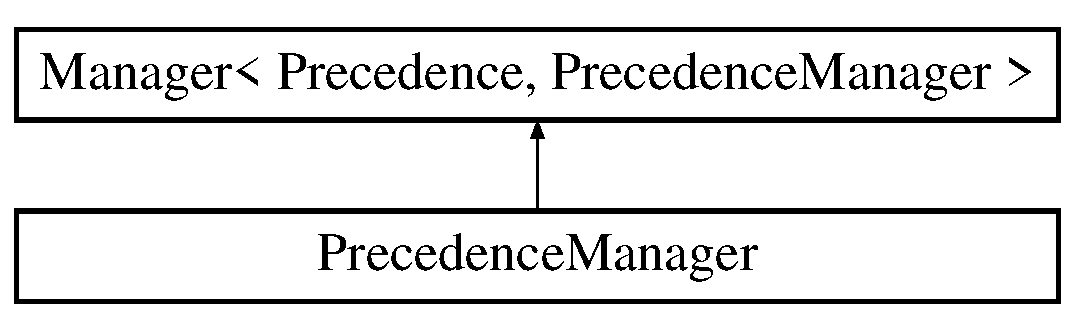
\includegraphics[height=2.000000cm]{class_precedence_manager}
\end{center}
\end{figure}
\subsection*{Fonctions membres publiques}
\begin{DoxyCompactItemize}
\item 
void \hyperlink{class_precedence_manager_ae59ff8a8e92d171c607e988d74a8fe1f}{delete\+Item} (\hyperlink{class_precedence}{Precedence} $\ast$t)
\item 
\hyperlink{class_precedence}{Precedence} \& \hyperlink{class_precedence_manager_ad8f271ddf75e6aa4b5a51eadaab662d0}{ajouter\+Precedence} (const \hyperlink{class_tache}{Tache} \&t1, const \hyperlink{class_tache}{Tache} \&t2)
\item 
\hypertarget{class_precedence_manager_acb5b927060191c478f496fbe30cd521d}{}void {\bfseries supprimer\+Precedence} (const Q\+String \&id)\label{class_precedence_manager_acb5b927060191c478f496fbe30cd521d}

\item 
bool \hyperlink{class_precedence_manager_ab50a623212a24469debe33e9df71037f}{is\+Predecesseur} (const \hyperlink{class_tache}{Tache} \&t1, const \hyperlink{class_tache}{Tache} \&t2) const 
\end{DoxyCompactItemize}
\subsection*{Membres hérités additionnels}


\subsection{Description détaillée}
La classe \hyperlink{class_precedence_manager}{Precedence\+Manager} est un \hyperlink{class_manager}{Manager} qui gère les items de type \hyperlink{class_precedence}{Precedence}. Elle ne peut être instanciée à cause du singleton mis en place dans sa classe mère. Elle peut toutefois être récupérée dans une référence ou un pointeur à l\textquotesingle{}aide la méthode mère\+: \hyperlink{class_manager_a8372e4f1e14f3605a57d839b152325ed}{get\+Instance()}. 

\subsection{Documentation des fonctions membres}
\hypertarget{class_precedence_manager_ad8f271ddf75e6aa4b5a51eadaab662d0}{}\index{Precedence\+Manager@{Precedence\+Manager}!ajouter\+Precedence@{ajouter\+Precedence}}
\index{ajouter\+Precedence@{ajouter\+Precedence}!Precedence\+Manager@{Precedence\+Manager}}
\subsubsection[{ajouter\+Precedence}]{\setlength{\rightskip}{0pt plus 5cm}{\bf Precedence} \& Precedence\+Manager\+::ajouter\+Precedence (
\begin{DoxyParamCaption}
\item[{const {\bf Tache} \&}]{t1, }
\item[{const {\bf Tache} \&}]{t2}
\end{DoxyParamCaption}
)}\label{class_precedence_manager_ad8f271ddf75e6aa4b5a51eadaab662d0}
Créer une une précédence entre deux tâches en vérifiant si celle-\/ci ne créera pas de circuit\+:
\begin{DoxyItemize}
\item La précédence de tâche1 est tâche2, la précédence de tâche2 est tâche1.
\end{DoxyItemize}

Puis l\textquotesingle{}ajoute au vecteur et renvoie sa référence. \hypertarget{class_precedence_manager_ae59ff8a8e92d171c607e988d74a8fe1f}{}\index{Precedence\+Manager@{Precedence\+Manager}!delete\+Item@{delete\+Item}}
\index{delete\+Item@{delete\+Item}!Precedence\+Manager@{Precedence\+Manager}}
\subsubsection[{delete\+Item}]{\setlength{\rightskip}{0pt plus 5cm}void Precedence\+Manager\+::delete\+Item (
\begin{DoxyParamCaption}
\item[{{\bf Precedence} $\ast$}]{t}
\end{DoxyParamCaption}
)}\label{class_precedence_manager_ae59ff8a8e92d171c607e988d74a8fe1f}
Supprimer la prédécence passée en paramètre. \hypertarget{class_precedence_manager_ab50a623212a24469debe33e9df71037f}{}\index{Precedence\+Manager@{Precedence\+Manager}!is\+Predecesseur@{is\+Predecesseur}}
\index{is\+Predecesseur@{is\+Predecesseur}!Precedence\+Manager@{Precedence\+Manager}}
\subsubsection[{is\+Predecesseur}]{\setlength{\rightskip}{0pt plus 5cm}bool Precedence\+Manager\+::is\+Predecesseur (
\begin{DoxyParamCaption}
\item[{const {\bf Tache} \&}]{t1, }
\item[{const {\bf Tache} \&}]{t2}
\end{DoxyParamCaption}
) const}\label{class_precedence_manager_ab50a623212a24469debe33e9df71037f}
Retourne vrai si tâche 1 est un prédécesseur de tâche 2. 

La documentation de cette classe a été générée à partir des fichiers suivants \+:\begin{DoxyCompactItemize}
\item 
manager.\+h\item 
manager.\+cpp\end{DoxyCompactItemize}

\hypertarget{class_programmation}{}\section{Référence de la classe Programmation}
\label{class_programmation}\index{Programmation@{Programmation}}


La classe \hyperlink{class_programmation}{Programmation} permet de programmer un évènement à une heure fixe en fonction de ses \hyperlink{class_precedence}{Precedence} s, de sa date de disponibilité et de sa date d\textquotesingle{}échéance. Une programmation ne peut être instanciée que par le biais du \hyperlink{class_programmation_manager}{Programmation\+Manager}.  




{\ttfamily \#include $<$evenement.\+h$>$}

\subsection*{Fonctions membres publiques}
\begin{DoxyCompactItemize}
\item 
\hyperlink{class_evenement}{Evenement} \& \hyperlink{class_programmation_a574f0e84ee4de3937249dff5df428d9a}{get\+Evenement} () const 
\item 
const Q\+Date\+Time \& \hyperlink{class_programmation_af047996948783353b99d55e2cd3dfd67}{get\+Date} () const 
\item 
Q\+Date\+Time \hyperlink{class_programmation_a178ae2552313a68a3552dea0782d042e}{get\+Fin} () const 
\item 
const \hyperlink{class_q_time_span}{Q\+Time\+Span} \& \hyperlink{class_programmation_a45fae841a66ff8abc7bd0af0d913f99f}{get\+Duree} () const 
\end{DoxyCompactItemize}
\subsection*{Amis}
\begin{DoxyCompactItemize}
\item 
\hypertarget{class_programmation_ade7bfcbf8cec66b12064c8ff25993d73}{}class {\bfseries Programmation\+Manager}\label{class_programmation_ade7bfcbf8cec66b12064c8ff25993d73}

\item 
\hypertarget{class_programmation_a2addbb7d8b656f2ebe9ca6edbb551f64}{}class {\bfseries Manager$<$ Programmation, Programmation\+Manager $>$}\label{class_programmation_a2addbb7d8b656f2ebe9ca6edbb551f64}

\end{DoxyCompactItemize}


\subsection{Description détaillée}
La classe \hyperlink{class_programmation}{Programmation} permet de programmer un évènement à une heure fixe en fonction de ses \hyperlink{class_precedence}{Precedence} s, de sa date de disponibilité et de sa date d\textquotesingle{}échéance. Une programmation ne peut être instanciée que par le biais du \hyperlink{class_programmation_manager}{Programmation\+Manager}. 

\subsection{Documentation des fonctions membres}
\hypertarget{class_programmation_af047996948783353b99d55e2cd3dfd67}{}\index{Programmation@{Programmation}!get\+Date@{get\+Date}}
\index{get\+Date@{get\+Date}!Programmation@{Programmation}}
\subsubsection[{get\+Date}]{\setlength{\rightskip}{0pt plus 5cm}const Q\+Date\+Time\& Programmation\+::get\+Date (
\begin{DoxyParamCaption}
{}
\end{DoxyParamCaption}
) const\hspace{0.3cm}{\ttfamily [inline]}}\label{class_programmation_af047996948783353b99d55e2cd3dfd67}
Renvoie la date de la programmation. \hypertarget{class_programmation_a45fae841a66ff8abc7bd0af0d913f99f}{}\index{Programmation@{Programmation}!get\+Duree@{get\+Duree}}
\index{get\+Duree@{get\+Duree}!Programmation@{Programmation}}
\subsubsection[{get\+Duree}]{\setlength{\rightskip}{0pt plus 5cm}const {\bf Q\+Time\+Span}\& Programmation\+::get\+Duree (
\begin{DoxyParamCaption}
{}
\end{DoxyParamCaption}
) const\hspace{0.3cm}{\ttfamily [inline]}}\label{class_programmation_a45fae841a66ff8abc7bd0af0d913f99f}
Renvoie la durée de la programmation. \hypertarget{class_programmation_a574f0e84ee4de3937249dff5df428d9a}{}\index{Programmation@{Programmation}!get\+Evenement@{get\+Evenement}}
\index{get\+Evenement@{get\+Evenement}!Programmation@{Programmation}}
\subsubsection[{get\+Evenement}]{\setlength{\rightskip}{0pt plus 5cm}{\bf Evenement}\& Programmation\+::get\+Evenement (
\begin{DoxyParamCaption}
{}
\end{DoxyParamCaption}
) const\hspace{0.3cm}{\ttfamily [inline]}}\label{class_programmation_a574f0e84ee4de3937249dff5df428d9a}
Renvoie l\textquotesingle{}évènement lié à la programmation. \hypertarget{class_programmation_a178ae2552313a68a3552dea0782d042e}{}\index{Programmation@{Programmation}!get\+Fin@{get\+Fin}}
\index{get\+Fin@{get\+Fin}!Programmation@{Programmation}}
\subsubsection[{get\+Fin}]{\setlength{\rightskip}{0pt plus 5cm}Q\+Date\+Time Programmation\+::get\+Fin (
\begin{DoxyParamCaption}
{}
\end{DoxyParamCaption}
) const\hspace{0.3cm}{\ttfamily [inline]}}\label{class_programmation_a178ae2552313a68a3552dea0782d042e}
Renvoie la date de fin de la programmation, calculée grâce à la durée et au début de celle-\/ci. 

La documentation de cette classe a été générée à partir du fichier suivant \+:\begin{DoxyCompactItemize}
\item 
evenement.\+h\end{DoxyCompactItemize}

\hypertarget{classprogrammation_activite}{}\section{Référence de la classe programmation\+Activite}
\label{classprogrammation_activite}\index{programmation\+Activite@{programmation\+Activite}}


Fenêtre d\textquotesingle{}ajout et de modification de \hyperlink{class_programmation}{Programmation} d\textquotesingle{}\hyperlink{class_activite}{Activite}.  




{\ttfamily \#include $<$programmationactivite.\+h$>$}

Graphe d\textquotesingle{}héritage de programmation\+Activite\+:\begin{figure}[H]
\begin{center}
\leavevmode
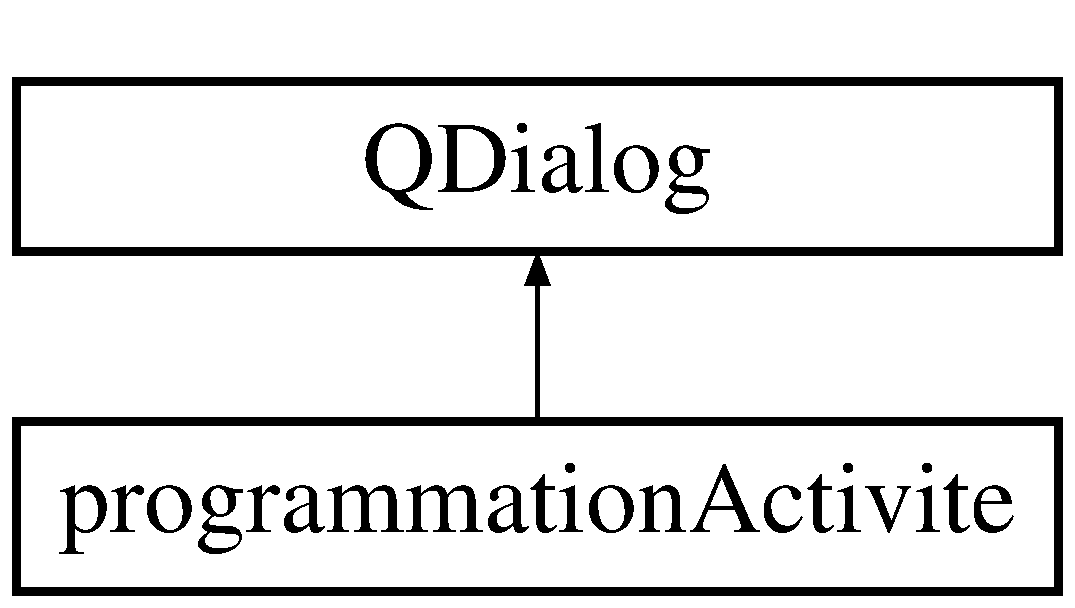
\includegraphics[height=2.000000cm]{classprogrammation_activite}
\end{center}
\end{figure}
\subsection*{Fonctions membres publiques}
\begin{DoxyCompactItemize}
\item 
\hypertarget{classprogrammation_activite_a10b94d6e981fa26f875ebdf464395148}{}{\bfseries programmation\+Activite} (\hyperlink{class_activite}{Activite} $\ast$activite, Q\+Widget $\ast$parent=0)\label{classprogrammation_activite_a10b94d6e981fa26f875ebdf464395148}

\end{DoxyCompactItemize}


\subsection{Description détaillée}
Fenêtre d\textquotesingle{}ajout et de modification de \hyperlink{class_programmation}{Programmation} d\textquotesingle{}\hyperlink{class_activite}{Activite}. 

La documentation de cette classe a été générée à partir des fichiers suivants \+:\begin{DoxyCompactItemize}
\item 
G\+U\+I/programmationactivite.\+h\item 
G\+U\+I/programmationactivite.\+cpp\end{DoxyCompactItemize}

\hypertarget{class_programmation_manager}{}\section{Référence de la classe Programmation\+Manager}
\label{class_programmation_manager}\index{Programmation\+Manager@{Programmation\+Manager}}


La classe \hyperlink{class_programmation_manager}{Programmation\+Manager} est un \hyperlink{class_manager}{Manager} qui gère les items de type \hyperlink{class_programmation}{Programmation}. Elle ne peut être instanciée à cause du singleton mis en place dans sa classe mère. Elle peut toutefois être récupérée dans une référence ou un pointeur à l\textquotesingle{}aide la méthode mère\+: \hyperlink{class_manager_a8372e4f1e14f3605a57d839b152325ed}{get\+Instance()}.  




{\ttfamily \#include $<$manager.\+h$>$}

Graphe d\textquotesingle{}héritage de Programmation\+Manager\+:\begin{figure}[H]
\begin{center}
\leavevmode
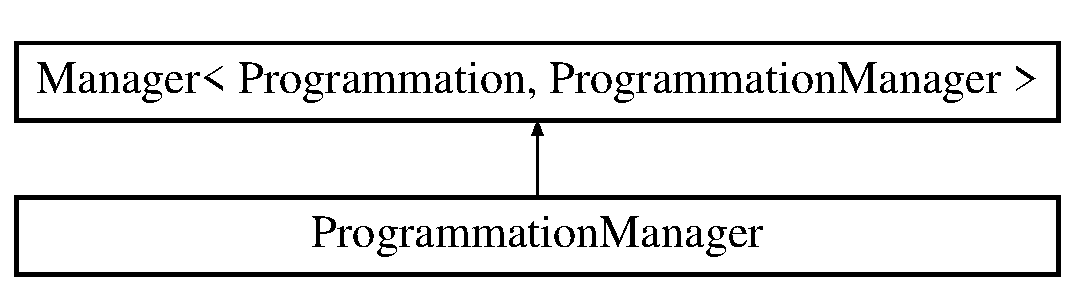
\includegraphics[height=2.000000cm]{class_programmation_manager}
\end{center}
\end{figure}
\subsection*{Fonctions membres publiques}
\begin{DoxyCompactItemize}
\item 
\hyperlink{class_programmation}{Programmation} \& \hyperlink{class_programmation_manager_acc7437f476ff946f81f676161b2e5d7a}{ajouter\+Programmation} (\hyperlink{class_evenement}{Evenement} \&evenement, const Q\+Date\+Time \&horaire, const \hyperlink{class_q_time_span}{Q\+Time\+Span} \&duree)
\item 
\hyperlink{class_programmation}{Programmation} \& \hyperlink{class_programmation_manager_a98ce96ec69b8df333648132fdb64840f}{ajouter\+Programmation} (\hyperlink{class_evenement}{Evenement} \&evenement, const Q\+String \&horaire, const Q\+String \&duree)
\item 
bool \hyperlink{class_programmation_manager_a55d24db8e1764ca3448e0451c6c9d211}{is\+Programmee} (const \hyperlink{class_evenement}{Evenement} \&e) const 
\item 
bool \hyperlink{class_programmation_manager_a4fae79fb6e160ca921b39060d9722c13}{is\+Programmee} (const \hyperlink{class_tache}{Tache} \&t, const Q\+Date\+Time \&date) const 
\item 
bool \hyperlink{class_programmation_manager_a17f660f90e17cfa6d87274644238ad74}{is\+Programmable} (const \hyperlink{class_evenement}{Evenement} \&t, const Q\+Date\+Time \&horaire, const \hyperlink{class_q_time_span}{Q\+Time\+Span} \&duree) const 
\item 
\hyperlink{class_q_time_span}{Q\+Time\+Span} \hyperlink{class_programmation_manager_a2f48066312a266f60c8b2b9bcf16b561}{duree\+Programmee} (const \hyperlink{class_evenement}{Evenement} \&e) const 
\item 
Q\+Date\+Time \hyperlink{class_programmation_manager_a808640afebdc24483826a1d3bc5d353a}{get\+Fin\+Tache} (const \hyperlink{class_tache_unitaire}{Tache\+Unitaire} \&tache) const 
\item 
vector$<$ const \hyperlink{class_programmation}{Programmation} $\ast$ $>$ \hyperlink{class_programmation_manager_a312930a36ef51d2d2e5b984438d57cd8}{get\+Programmations} (const \hyperlink{class_tache_unitaire}{Tache\+Unitaire} \&tache) const 
\item 
const vector$<$ \hyperlink{class_programmation}{Programmation} $\ast$ $>$ \hyperlink{class_programmation_manager_a3eea8e9a8f5d63e49e7a380d68272ff1}{get\+Programmations} (int week, int year) const 
\item 
\hyperlink{class_programmation}{Programmation} $\ast$ \hyperlink{class_programmation_manager_ad5f64c40cc00911159d5faf75b71deb1}{get\+Programmation} (const Q\+Date\+Time \&date) const 
\item 
void \hyperlink{class_programmation_manager_a640212a0312d5a83988c91f8673ea51b}{delete\+Item} (\hyperlink{class_programmation}{Programmation} $\ast$p)
\end{DoxyCompactItemize}
\subsection*{Membres hérités additionnels}


\subsection{Description détaillée}
La classe \hyperlink{class_programmation_manager}{Programmation\+Manager} est un \hyperlink{class_manager}{Manager} qui gère les items de type \hyperlink{class_programmation}{Programmation}. Elle ne peut être instanciée à cause du singleton mis en place dans sa classe mère. Elle peut toutefois être récupérée dans une référence ou un pointeur à l\textquotesingle{}aide la méthode mère\+: \hyperlink{class_manager_a8372e4f1e14f3605a57d839b152325ed}{get\+Instance()}. 

\subsection{Documentation des fonctions membres}
\hypertarget{class_programmation_manager_acc7437f476ff946f81f676161b2e5d7a}{}\index{Programmation\+Manager@{Programmation\+Manager}!ajouter\+Programmation@{ajouter\+Programmation}}
\index{ajouter\+Programmation@{ajouter\+Programmation}!Programmation\+Manager@{Programmation\+Manager}}
\subsubsection[{ajouter\+Programmation}]{\setlength{\rightskip}{0pt plus 5cm}{\bf Programmation} \& Programmation\+Manager\+::ajouter\+Programmation (
\begin{DoxyParamCaption}
\item[{{\bf Evenement} \&}]{evenement, }
\item[{const Q\+Date\+Time \&}]{horaire, }
\item[{const {\bf Q\+Time\+Span} \&}]{duree}
\end{DoxyParamCaption}
)}\label{class_programmation_manager_acc7437f476ff946f81f676161b2e5d7a}
Créer une programmation d\textquotesingle{}évènement en vérifiant les attributs passés en paramètre et si la tâche est bien programmable. Puis l\textquotesingle{}ajoute au vecteur et renvoie sa référence. \hypertarget{class_programmation_manager_a98ce96ec69b8df333648132fdb64840f}{}\index{Programmation\+Manager@{Programmation\+Manager}!ajouter\+Programmation@{ajouter\+Programmation}}
\index{ajouter\+Programmation@{ajouter\+Programmation}!Programmation\+Manager@{Programmation\+Manager}}
\subsubsection[{ajouter\+Programmation}]{\setlength{\rightskip}{0pt plus 5cm}{\bf Programmation} \& Programmation\+Manager\+::ajouter\+Programmation (
\begin{DoxyParamCaption}
\item[{{\bf Evenement} \&}]{evenement, }
\item[{const Q\+String \&}]{horaire, }
\item[{const Q\+String \&}]{duree}
\end{DoxyParamCaption}
)}\label{class_programmation_manager_a98ce96ec69b8df333648132fdb64840f}
Créer un projet en vérifiant les attributs passés en paramètre. Puis l\textquotesingle{}ajoute au vecteur et renvoie sa référence. \hypertarget{class_programmation_manager_a640212a0312d5a83988c91f8673ea51b}{}\index{Programmation\+Manager@{Programmation\+Manager}!delete\+Item@{delete\+Item}}
\index{delete\+Item@{delete\+Item}!Programmation\+Manager@{Programmation\+Manager}}
\subsubsection[{delete\+Item}]{\setlength{\rightskip}{0pt plus 5cm}void Programmation\+Manager\+::delete\+Item (
\begin{DoxyParamCaption}
\item[{{\bf Programmation} $\ast$}]{p}
\end{DoxyParamCaption}
)}\label{class_programmation_manager_a640212a0312d5a83988c91f8673ea51b}
Supprime la programmation passée en paramètre. \hypertarget{class_programmation_manager_a2f48066312a266f60c8b2b9bcf16b561}{}\index{Programmation\+Manager@{Programmation\+Manager}!duree\+Programmee@{duree\+Programmee}}
\index{duree\+Programmee@{duree\+Programmee}!Programmation\+Manager@{Programmation\+Manager}}
\subsubsection[{duree\+Programmee}]{\setlength{\rightskip}{0pt plus 5cm}{\bf Q\+Time\+Span} Programmation\+Manager\+::duree\+Programmee (
\begin{DoxyParamCaption}
\item[{const {\bf Evenement} \&}]{e}
\end{DoxyParamCaption}
) const}\label{class_programmation_manager_a2f48066312a266f60c8b2b9bcf16b561}
Renvoie la durée totale programmée de l\textquotesingle{}évènement, si celui-\/ci est préemptif (dans le cas d\textquotesingle{}une tâche unitaire préemptive) ou non. \hypertarget{class_programmation_manager_a808640afebdc24483826a1d3bc5d353a}{}\index{Programmation\+Manager@{Programmation\+Manager}!get\+Fin\+Tache@{get\+Fin\+Tache}}
\index{get\+Fin\+Tache@{get\+Fin\+Tache}!Programmation\+Manager@{Programmation\+Manager}}
\subsubsection[{get\+Fin\+Tache}]{\setlength{\rightskip}{0pt plus 5cm}Q\+Date\+Time Programmation\+Manager\+::get\+Fin\+Tache (
\begin{DoxyParamCaption}
\item[{const {\bf Tache\+Unitaire} \&}]{tache}
\end{DoxyParamCaption}
) const}\label{class_programmation_manager_a808640afebdc24483826a1d3bc5d353a}
Renvoie la date de fin de la tâche. \hypertarget{class_programmation_manager_ad5f64c40cc00911159d5faf75b71deb1}{}\index{Programmation\+Manager@{Programmation\+Manager}!get\+Programmation@{get\+Programmation}}
\index{get\+Programmation@{get\+Programmation}!Programmation\+Manager@{Programmation\+Manager}}
\subsubsection[{get\+Programmation}]{\setlength{\rightskip}{0pt plus 5cm}{\bf Programmation} $\ast$ Programmation\+Manager\+::get\+Programmation (
\begin{DoxyParamCaption}
\item[{const Q\+Date\+Time \&}]{date}
\end{DoxyParamCaption}
) const}\label{class_programmation_manager_ad5f64c40cc00911159d5faf75b71deb1}
Renvoie la programmation d\textquotesingle{}un évènement quelconque dont la date de programmation est celle passée en paramètre. (une unique programmation peut avoir lieu en un temps donné) \hypertarget{class_programmation_manager_a312930a36ef51d2d2e5b984438d57cd8}{}\index{Programmation\+Manager@{Programmation\+Manager}!get\+Programmations@{get\+Programmations}}
\index{get\+Programmations@{get\+Programmations}!Programmation\+Manager@{Programmation\+Manager}}
\subsubsection[{get\+Programmations}]{\setlength{\rightskip}{0pt plus 5cm}vector$<$ const {\bf Programmation} $\ast$ $>$ Programmation\+Manager\+::get\+Programmations (
\begin{DoxyParamCaption}
\item[{const {\bf Tache\+Unitaire} \&}]{tache}
\end{DoxyParamCaption}
) const}\label{class_programmation_manager_a312930a36ef51d2d2e5b984438d57cd8}
Retourne un vecteur de pointeurs des programmations liées à une tâche unitaire.
\begin{DoxyItemize}
\item Si la tâche n\textquotesingle{}est pas programmée, elle renvoie un vecteur vide.
\item Si la tâche est programmée et non-\/préemptive, elle renvoie un vecteur contenant un seul pointeur de programmation.
\item Si la tâche est programmée et préemptive, elle renvoie un vecteur contenant tous les pointeurs de programmation. 
\end{DoxyItemize}\hypertarget{class_programmation_manager_a3eea8e9a8f5d63e49e7a380d68272ff1}{}\index{Programmation\+Manager@{Programmation\+Manager}!get\+Programmations@{get\+Programmations}}
\index{get\+Programmations@{get\+Programmations}!Programmation\+Manager@{Programmation\+Manager}}
\subsubsection[{get\+Programmations}]{\setlength{\rightskip}{0pt plus 5cm}const vector$<$ {\bf Programmation} $\ast$ $>$ Programmation\+Manager\+::get\+Programmations (
\begin{DoxyParamCaption}
\item[{int}]{week, }
\item[{int}]{year}
\end{DoxyParamCaption}
) const}\label{class_programmation_manager_a3eea8e9a8f5d63e49e7a380d68272ff1}
Retourne un vecteur de pointeurs des programmations qui ont lieu lors de la semaine et de l\textquotesingle{}année passées en paramètre. \hypertarget{class_programmation_manager_a17f660f90e17cfa6d87274644238ad74}{}\index{Programmation\+Manager@{Programmation\+Manager}!is\+Programmable@{is\+Programmable}}
\index{is\+Programmable@{is\+Programmable}!Programmation\+Manager@{Programmation\+Manager}}
\subsubsection[{is\+Programmable}]{\setlength{\rightskip}{0pt plus 5cm}bool Programmation\+Manager\+::is\+Programmable (
\begin{DoxyParamCaption}
\item[{const {\bf Evenement} \&}]{t, }
\item[{const Q\+Date\+Time \&}]{horaire, }
\item[{const {\bf Q\+Time\+Span} \&}]{duree}
\end{DoxyParamCaption}
) const}\label{class_programmation_manager_a17f660f90e17cfa6d87274644238ad74}
Vérifie les contraintes liées la date de disponibilité, d\textquotesingle{}échéance, la durée, aux précédence et au projet lié. Retourne vrai si toutes ces contraintes sont vérifiées. \hypertarget{class_programmation_manager_a55d24db8e1764ca3448e0451c6c9d211}{}\index{Programmation\+Manager@{Programmation\+Manager}!is\+Programmee@{is\+Programmee}}
\index{is\+Programmee@{is\+Programmee}!Programmation\+Manager@{Programmation\+Manager}}
\subsubsection[{is\+Programmee}]{\setlength{\rightskip}{0pt plus 5cm}bool Programmation\+Manager\+::is\+Programmee (
\begin{DoxyParamCaption}
\item[{const {\bf Evenement} \&}]{e}
\end{DoxyParamCaption}
) const}\label{class_programmation_manager_a55d24db8e1764ca3448e0451c6c9d211}
Renvoie vrai si l\textquotesingle{}évènement est entièrement programmé. Dans le cas d\textquotesingle{}une tâche préemptive, is\+Programmee retournera vrai si elle est entièrement programmée. Renvoie faux le cas échéant. \hypertarget{class_programmation_manager_a4fae79fb6e160ca921b39060d9722c13}{}\index{Programmation\+Manager@{Programmation\+Manager}!is\+Programmee@{is\+Programmee}}
\index{is\+Programmee@{is\+Programmee}!Programmation\+Manager@{Programmation\+Manager}}
\subsubsection[{is\+Programmee}]{\setlength{\rightskip}{0pt plus 5cm}bool Programmation\+Manager\+::is\+Programmee (
\begin{DoxyParamCaption}
\item[{const {\bf Tache} \&}]{t, }
\item[{const Q\+Date\+Time \&}]{date}
\end{DoxyParamCaption}
) const}\label{class_programmation_manager_a4fae79fb6e160ca921b39060d9722c13}
Renvoie vrai si l\textquotesingle{}évènement est entièrement programmé. Dans le cas d\textquotesingle{}une tâche préemptive, is\+Programmee retournera vrai si elle est entièrement programmée. Renvoie faux le cas échéant. 

La documentation de cette classe a été générée à partir des fichiers suivants \+:\begin{DoxyCompactItemize}
\item 
manager.\+h\item 
manager.\+cpp\end{DoxyCompactItemize}

\hypertarget{classprogrammation_tache}{}\section{Référence de la classe programmation\+Tache}
\label{classprogrammation_tache}\index{programmation\+Tache@{programmation\+Tache}}


Fenêtre d\textquotesingle{}ajout et de modification de \hyperlink{class_programmation}{Programmation} de \hyperlink{class_tache}{Tache}.  




{\ttfamily \#include $<$programmationtache.\+h$>$}

Graphe d\textquotesingle{}héritage de programmation\+Tache\+:\begin{figure}[H]
\begin{center}
\leavevmode
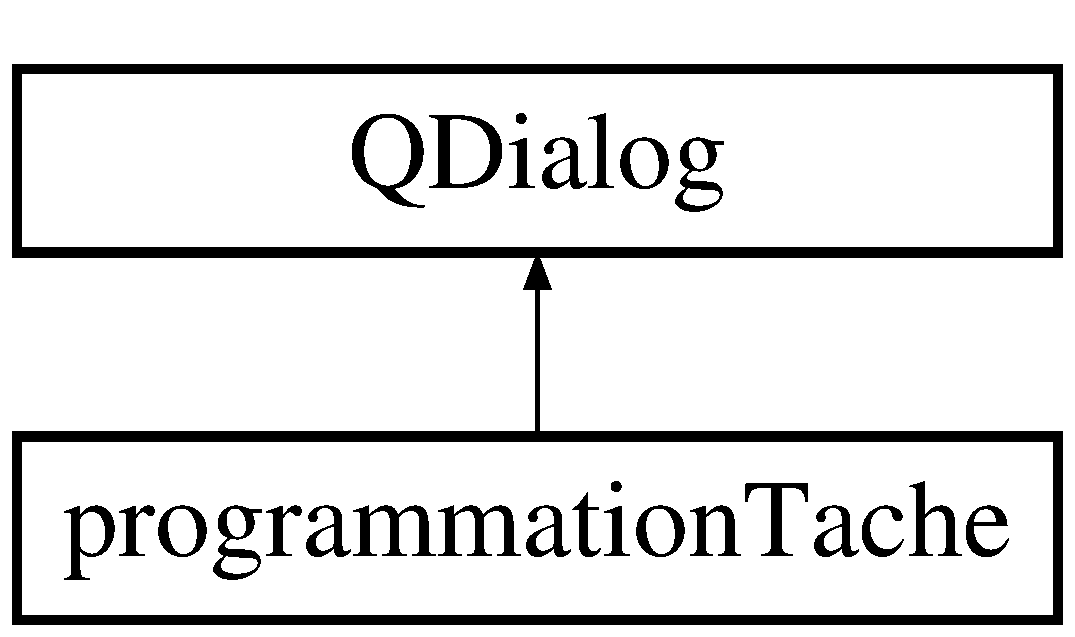
\includegraphics[height=2.000000cm]{classprogrammation_tache}
\end{center}
\end{figure}
\subsection*{Fonctions membres publiques}
\begin{DoxyCompactItemize}
\item 
\hypertarget{classprogrammation_tache_a95f013eeff1cffc8ce6b30cc31b8df68}{}{\bfseries programmation\+Tache} (\hyperlink{class_tache_unitaire}{Tache\+Unitaire} $\ast$tache=0, Q\+Widget $\ast$parent=0)\label{classprogrammation_tache_a95f013eeff1cffc8ce6b30cc31b8df68}

\end{DoxyCompactItemize}


\subsection{Description détaillée}
Fenêtre d\textquotesingle{}ajout et de modification de \hyperlink{class_programmation}{Programmation} de \hyperlink{class_tache}{Tache}. 

La documentation de cette classe a été générée à partir des fichiers suivants \+:\begin{DoxyCompactItemize}
\item 
G\+U\+I/programmationtache.\+h\item 
G\+U\+I/programmationtache.\+cpp\end{DoxyCompactItemize}

\hypertarget{class_projet}{}\section{Référence de la classe Projet}
\label{class_projet}\index{Projet@{Projet}}


La classe \hyperlink{class_projet}{Projet} permet de regrouper différentes Taches et impose une dâte de disponibilité. Elle ne peut être instanciée que par le biais du \hyperlink{class_projet_manager}{Projet\+Manager}.  




{\ttfamily \#include $<$evenement.\+h$>$}

\subsection*{Classes}
\begin{DoxyCompactItemize}
\item 
class \hyperlink{class_projet_1_1const__iterator}{const\+\_\+iterator}
\item 
class \hyperlink{class_projet_1_1iterator}{iterator}
\end{DoxyCompactItemize}
\subsection*{Fonctions membres publiques}
\begin{DoxyCompactItemize}
\item 
\hyperlink{class_projet_1_1iterator}{iterator} \hyperlink{class_projet_a8d7cc0246df8b6929f4798b1024e208d}{begin} ()
\item 
\hyperlink{class_projet_1_1iterator}{iterator} \hyperlink{class_projet_a2aeb5e7db79a1240800d91b962c14ddf}{end} ()
\item 
\hyperlink{class_projet_1_1const__iterator}{const\+\_\+iterator} \hyperlink{class_projet_a16cb2ae4625deab305145f78db918e59}{begin} () const 
\item 
\hyperlink{class_projet_1_1const__iterator}{const\+\_\+iterator} \hyperlink{class_projet_ab24984c532525679fe3c0230b0686363}{end} () const 
\item 
size\+\_\+t \hyperlink{class_projet_aaa4fac44323bd319c740c1f1d285bfaa}{get\+Size} () const 
\item 
const Q\+Date\+Time \& \hyperlink{class_projet_a0deffe9e90675158ea636d346d454cc1}{get\+Disponibilite} () const 
\item 
Q\+Date\+Time \hyperlink{class_projet_aaf16b2ced20117743bee25d546f11f78}{get\+Echeance} ()
\item 
const Q\+String \& \hyperlink{class_projet_a917a74942a7c232849012687dad64b8e}{get\+Titre} () const 
\item 
const Q\+String \& \hyperlink{class_projet_a9a92a64fdf15130c72e3d4a9875467f0}{get\+Id} () const 
\item 
bool \hyperlink{class_projet_a42363da876b04e6028924fba9e2e86d8}{possede} (const \hyperlink{class_tache}{Tache} \&t)
\item 
void \hyperlink{class_projet_a5f325c588558b085ffacf51c48f06551}{set\+Id} (const Q\+String \&i)
\item 
void \hyperlink{class_projet_a1bc00f170040b45948f34b3ce7e0642b}{set\+Titre} (const Q\+String \&t)
\item 
void \hyperlink{class_projet_aba69d4166df2f8dc32e39913f2add7f2}{set\+Disponibilite} (const Q\+Date\+Time \&t)
\item 
void \hyperlink{class_projet_adf4f7c0f48ee4661b57be82af2b056ae}{ajouter\+Tache} (\hyperlink{class_tache}{Tache} $\ast$t)
\item 
void \hyperlink{class_projet_a65c346c033545bf02e08864c16ae2e8f}{ajouter\+Tache} (const Q\+String \&id)
\item 
void \hyperlink{class_projet_a3c0c1f9a620854878291c3e873a52f6e}{retirer\+Tache} (\hyperlink{class_tache}{Tache} $\ast$t)
\item 
void \hyperlink{class_projet_a9cc9037c1ee3ab49a1cbf3c153665f19}{retirer\+Tache} (const Q\+String \&id)
\item 
virtual void \hyperlink{class_projet_aff670a5010d70339cdce91773f7199a3}{afficher} ()
\end{DoxyCompactItemize}
\subsection*{Amis}
\begin{DoxyCompactItemize}
\item 
\hypertarget{class_projet_aaaed9857b3481233fa7c581b5c86151d}{}class {\bfseries Projet\+Manager}\label{class_projet_aaaed9857b3481233fa7c581b5c86151d}

\item 
\hypertarget{class_projet_a8cf00d1da3b93cadfd9c400c941b9b73}{}class {\bfseries Manager$<$ Projet, Projet\+Manager $>$}\label{class_projet_a8cf00d1da3b93cadfd9c400c941b9b73}

\end{DoxyCompactItemize}


\subsection{Description détaillée}
La classe \hyperlink{class_projet}{Projet} permet de regrouper différentes Taches et impose une dâte de disponibilité. Elle ne peut être instanciée que par le biais du \hyperlink{class_projet_manager}{Projet\+Manager}. 

\subsection{Documentation des fonctions membres}
\hypertarget{class_projet_aff670a5010d70339cdce91773f7199a3}{}\index{Projet@{Projet}!afficher@{afficher}}
\index{afficher@{afficher}!Projet@{Projet}}
\subsubsection[{afficher}]{\setlength{\rightskip}{0pt plus 5cm}void Projet\+::afficher (
\begin{DoxyParamCaption}
{}
\end{DoxyParamCaption}
)\hspace{0.3cm}{\ttfamily [virtual]}}\label{class_projet_aff670a5010d70339cdce91773f7199a3}
La méthode \hyperlink{class_projet_aff670a5010d70339cdce91773f7199a3}{afficher()} permet d\textquotesingle{}afficher en mode debug les attributs et les tâches du projet.\hypertarget{class_projet_adf4f7c0f48ee4661b57be82af2b056ae}{}\index{Projet@{Projet}!ajouter\+Tache@{ajouter\+Tache}}
\index{ajouter\+Tache@{ajouter\+Tache}!Projet@{Projet}}
\subsubsection[{ajouter\+Tache}]{\setlength{\rightskip}{0pt plus 5cm}void Projet\+::ajouter\+Tache (
\begin{DoxyParamCaption}
\item[{{\bf Tache} $\ast$}]{t}
\end{DoxyParamCaption}
)}\label{class_projet_adf4f7c0f48ee4661b57be82af2b056ae}
La méthode \hyperlink{class_projet_adf4f7c0f48ee4661b57be82af2b056ae}{ajouter\+Tache()} ajoute la tâche correspondante dans le projet.\hypertarget{class_projet_a65c346c033545bf02e08864c16ae2e8f}{}\index{Projet@{Projet}!ajouter\+Tache@{ajouter\+Tache}}
\index{ajouter\+Tache@{ajouter\+Tache}!Projet@{Projet}}
\subsubsection[{ajouter\+Tache}]{\setlength{\rightskip}{0pt plus 5cm}void Projet\+::ajouter\+Tache (
\begin{DoxyParamCaption}
\item[{const Q\+String \&}]{id}
\end{DoxyParamCaption}
)}\label{class_projet_a65c346c033545bf02e08864c16ae2e8f}
Voir \hyperlink{class_projet_adf4f7c0f48ee4661b57be82af2b056ae}{ajouter\+Tache(\+Tache$\ast$ t)};\hypertarget{class_projet_a8d7cc0246df8b6929f4798b1024e208d}{}\index{Projet@{Projet}!begin@{begin}}
\index{begin@{begin}!Projet@{Projet}}
\subsubsection[{begin}]{\setlength{\rightskip}{0pt plus 5cm}{\bf iterator} Projet\+::begin (
\begin{DoxyParamCaption}
{}
\end{DoxyParamCaption}
)\hspace{0.3cm}{\ttfamily [inline]}}\label{class_projet_a8d7cc0246df8b6929f4798b1024e208d}
Renvoie un iterator sur la première tâche composante. \hypertarget{class_projet_a16cb2ae4625deab305145f78db918e59}{}\index{Projet@{Projet}!begin@{begin}}
\index{begin@{begin}!Projet@{Projet}}
\subsubsection[{begin}]{\setlength{\rightskip}{0pt plus 5cm}{\bf const\+\_\+iterator} Projet\+::begin (
\begin{DoxyParamCaption}
{}
\end{DoxyParamCaption}
) const\hspace{0.3cm}{\ttfamily [inline]}}\label{class_projet_a16cb2ae4625deab305145f78db918e59}
Renvoie un \hyperlink{class_projet_1_1const__iterator}{const\+\_\+iterator} sur la première tâche composante. \hypertarget{class_projet_a2aeb5e7db79a1240800d91b962c14ddf}{}\index{Projet@{Projet}!end@{end}}
\index{end@{end}!Projet@{Projet}}
\subsubsection[{end}]{\setlength{\rightskip}{0pt plus 5cm}{\bf iterator} Projet\+::end (
\begin{DoxyParamCaption}
{}
\end{DoxyParamCaption}
)\hspace{0.3cm}{\ttfamily [inline]}}\label{class_projet_a2aeb5e7db79a1240800d91b962c14ddf}
Renvoie un iterator sur la fin du tableau de tâches composantes. \hypertarget{class_projet_ab24984c532525679fe3c0230b0686363}{}\index{Projet@{Projet}!end@{end}}
\index{end@{end}!Projet@{Projet}}
\subsubsection[{end}]{\setlength{\rightskip}{0pt plus 5cm}{\bf const\+\_\+iterator} Projet\+::end (
\begin{DoxyParamCaption}
{}
\end{DoxyParamCaption}
) const\hspace{0.3cm}{\ttfamily [inline]}}\label{class_projet_ab24984c532525679fe3c0230b0686363}
Renvoie un \hyperlink{class_projet_1_1const__iterator}{const\+\_\+iterator} sur la fin du tableau de tâches composantes. \hypertarget{class_projet_a0deffe9e90675158ea636d346d454cc1}{}\index{Projet@{Projet}!get\+Disponibilite@{get\+Disponibilite}}
\index{get\+Disponibilite@{get\+Disponibilite}!Projet@{Projet}}
\subsubsection[{get\+Disponibilite}]{\setlength{\rightskip}{0pt plus 5cm}const Q\+Date\+Time\& Projet\+::get\+Disponibilite (
\begin{DoxyParamCaption}
{}
\end{DoxyParamCaption}
) const\hspace{0.3cm}{\ttfamily [inline]}}\label{class_projet_a0deffe9e90675158ea636d346d454cc1}
Renvoie la date de disponibilité du projet. \hypertarget{class_projet_aaf16b2ced20117743bee25d546f11f78}{}\index{Projet@{Projet}!get\+Echeance@{get\+Echeance}}
\index{get\+Echeance@{get\+Echeance}!Projet@{Projet}}
\subsubsection[{get\+Echeance}]{\setlength{\rightskip}{0pt plus 5cm}Q\+Date\+Time Projet\+::get\+Echeance (
\begin{DoxyParamCaption}
{}
\end{DoxyParamCaption}
)}\label{class_projet_aaf16b2ced20117743bee25d546f11f78}
La méthode \hyperlink{class_projet_aaf16b2ced20117743bee25d546f11f78}{get\+Echeance()} renvoie la date d\textquotesingle{}échéance la plus lointaine parmi celles des tâches qui composent le projet..\hypertarget{class_projet_a9a92a64fdf15130c72e3d4a9875467f0}{}\index{Projet@{Projet}!get\+Id@{get\+Id}}
\index{get\+Id@{get\+Id}!Projet@{Projet}}
\subsubsection[{get\+Id}]{\setlength{\rightskip}{0pt plus 5cm}const Q\+String\& Projet\+::get\+Id (
\begin{DoxyParamCaption}
{}
\end{DoxyParamCaption}
) const\hspace{0.3cm}{\ttfamily [inline]}}\label{class_projet_a9a92a64fdf15130c72e3d4a9875467f0}
Renvoie l\textquotesingle{}identificateur du projet. \hypertarget{class_projet_aaa4fac44323bd319c740c1f1d285bfaa}{}\index{Projet@{Projet}!get\+Size@{get\+Size}}
\index{get\+Size@{get\+Size}!Projet@{Projet}}
\subsubsection[{get\+Size}]{\setlength{\rightskip}{0pt plus 5cm}size\+\_\+t Projet\+::get\+Size (
\begin{DoxyParamCaption}
{}
\end{DoxyParamCaption}
) const\hspace{0.3cm}{\ttfamily [inline]}}\label{class_projet_aaa4fac44323bd319c740c1f1d285bfaa}
Renvoie le nombre de tâches liées au projet. \hypertarget{class_projet_a917a74942a7c232849012687dad64b8e}{}\index{Projet@{Projet}!get\+Titre@{get\+Titre}}
\index{get\+Titre@{get\+Titre}!Projet@{Projet}}
\subsubsection[{get\+Titre}]{\setlength{\rightskip}{0pt plus 5cm}const Q\+String\& Projet\+::get\+Titre (
\begin{DoxyParamCaption}
{}
\end{DoxyParamCaption}
) const\hspace{0.3cm}{\ttfamily [inline]}}\label{class_projet_a917a74942a7c232849012687dad64b8e}
Renvoie le titre du projet. \hypertarget{class_projet_a42363da876b04e6028924fba9e2e86d8}{}\index{Projet@{Projet}!possede@{possede}}
\index{possede@{possede}!Projet@{Projet}}
\subsubsection[{possede}]{\setlength{\rightskip}{0pt plus 5cm}bool Projet\+::possede (
\begin{DoxyParamCaption}
\item[{const {\bf Tache} \&}]{t}
\end{DoxyParamCaption}
)}\label{class_projet_a42363da876b04e6028924fba9e2e86d8}
La méthode \hyperlink{class_projet_a42363da876b04e6028924fba9e2e86d8}{possede()} renvoie true si le la tache en paramètre est liée au projet. False sinon.\hypertarget{class_projet_a3c0c1f9a620854878291c3e873a52f6e}{}\index{Projet@{Projet}!retirer\+Tache@{retirer\+Tache}}
\index{retirer\+Tache@{retirer\+Tache}!Projet@{Projet}}
\subsubsection[{retirer\+Tache}]{\setlength{\rightskip}{0pt plus 5cm}void Projet\+::retirer\+Tache (
\begin{DoxyParamCaption}
\item[{{\bf Tache} $\ast$}]{t}
\end{DoxyParamCaption}
)}\label{class_projet_a3c0c1f9a620854878291c3e873a52f6e}
La méthode \hyperlink{class_projet_a3c0c1f9a620854878291c3e873a52f6e}{retirer\+Tache()} retire la tâche correspondante du projet.\hypertarget{class_projet_a9cc9037c1ee3ab49a1cbf3c153665f19}{}\index{Projet@{Projet}!retirer\+Tache@{retirer\+Tache}}
\index{retirer\+Tache@{retirer\+Tache}!Projet@{Projet}}
\subsubsection[{retirer\+Tache}]{\setlength{\rightskip}{0pt plus 5cm}void Projet\+::retirer\+Tache (
\begin{DoxyParamCaption}
\item[{const Q\+String \&}]{id}
\end{DoxyParamCaption}
)}\label{class_projet_a9cc9037c1ee3ab49a1cbf3c153665f19}
Voir \hyperlink{class_projet_a3c0c1f9a620854878291c3e873a52f6e}{retirer\+Tache(\+Tache$\ast$ t)};\hypertarget{class_projet_aba69d4166df2f8dc32e39913f2add7f2}{}\index{Projet@{Projet}!set\+Disponibilite@{set\+Disponibilite}}
\index{set\+Disponibilite@{set\+Disponibilite}!Projet@{Projet}}
\subsubsection[{set\+Disponibilite}]{\setlength{\rightskip}{0pt plus 5cm}void Projet\+::set\+Disponibilite (
\begin{DoxyParamCaption}
\item[{const Q\+Date\+Time \&}]{t}
\end{DoxyParamCaption}
)\hspace{0.3cm}{\ttfamily [inline]}}\label{class_projet_aba69d4166df2f8dc32e39913f2add7f2}
Met à jour la date de disponibilité du projet. \hypertarget{class_projet_a5f325c588558b085ffacf51c48f06551}{}\index{Projet@{Projet}!set\+Id@{set\+Id}}
\index{set\+Id@{set\+Id}!Projet@{Projet}}
\subsubsection[{set\+Id}]{\setlength{\rightskip}{0pt plus 5cm}void Projet\+::set\+Id (
\begin{DoxyParamCaption}
\item[{const Q\+String \&}]{i}
\end{DoxyParamCaption}
)\hspace{0.3cm}{\ttfamily [inline]}}\label{class_projet_a5f325c588558b085ffacf51c48f06551}
Met à jour l\textquotesingle{}identificateur du projet. \hypertarget{class_projet_a1bc00f170040b45948f34b3ce7e0642b}{}\index{Projet@{Projet}!set\+Titre@{set\+Titre}}
\index{set\+Titre@{set\+Titre}!Projet@{Projet}}
\subsubsection[{set\+Titre}]{\setlength{\rightskip}{0pt plus 5cm}void Projet\+::set\+Titre (
\begin{DoxyParamCaption}
\item[{const Q\+String \&}]{t}
\end{DoxyParamCaption}
)\hspace{0.3cm}{\ttfamily [inline]}}\label{class_projet_a1bc00f170040b45948f34b3ce7e0642b}
Met à jour le titre du projet. 

La documentation de cette classe a été générée à partir des fichiers suivants \+:\begin{DoxyCompactItemize}
\item 
evenement.\+h\item 
evenement.\+cpp\end{DoxyCompactItemize}

\hypertarget{class_projet_manager}{}\section{Référence de la classe Projet\+Manager}
\label{class_projet_manager}\index{Projet\+Manager@{Projet\+Manager}}


La classe \hyperlink{class_projet_manager}{Projet\+Manager} est un \hyperlink{class_manager}{Manager} qui gère les items de type \hyperlink{class_projet}{Projet}. Elle ne peut être instanciée à cause du singleton mis en place dans sa classe mère. Elle peut toutefois être récupérée dans une référence ou un pointeur à l\textquotesingle{}aide la méthode mère\+: \hyperlink{class_manager_a8372e4f1e14f3605a57d839b152325ed}{get\+Instance()}.  




{\ttfamily \#include $<$manager.\+h$>$}

Graphe d\textquotesingle{}héritage de Projet\+Manager\+:\begin{figure}[H]
\begin{center}
\leavevmode
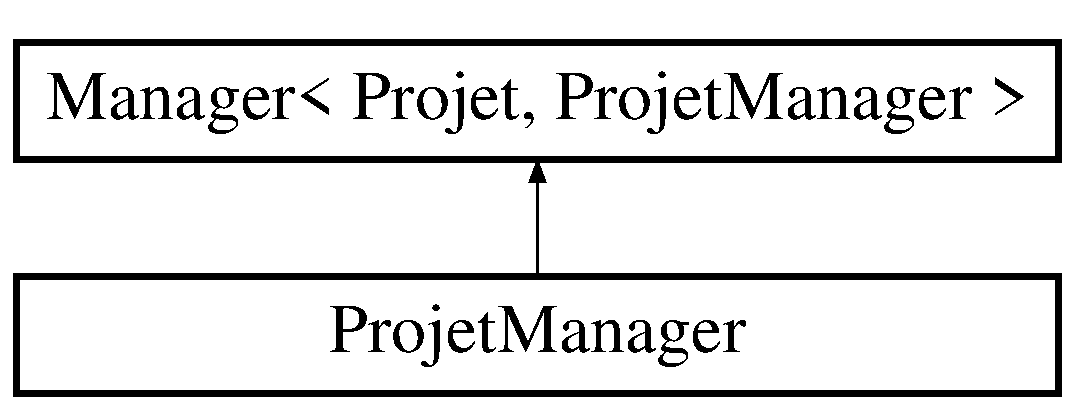
\includegraphics[height=2.000000cm]{class_projet_manager}
\end{center}
\end{figure}
\subsection*{Fonctions membres publiques}
\begin{DoxyCompactItemize}
\item 
\hyperlink{class_projet}{Projet} \& \hyperlink{class_projet_manager_a3394d5ab0749ea68efb5ae535b27e6fc}{ajouter\+Projet} (const Q\+String \&id, const Q\+String \&titre, const Q\+String \&dispo)
\item 
\hyperlink{class_projet}{Projet} \& \hyperlink{class_projet_manager_a6da5a61e20cbf0a6bc98a3681f977829}{ajouter\+Projet} (const Q\+String \&id, const Q\+String \&titre, const Q\+Date\+Time \&dispo)
\item 
\hypertarget{class_projet_manager_a04c4b5b2c4d84f2ad48abe24d6960607}{}void {\bfseries supprimer\+Projet} (Q\+String id)\label{class_projet_manager_a04c4b5b2c4d84f2ad48abe24d6960607}

\end{DoxyCompactItemize}
\subsection*{Membres hérités additionnels}


\subsection{Description détaillée}
La classe \hyperlink{class_projet_manager}{Projet\+Manager} est un \hyperlink{class_manager}{Manager} qui gère les items de type \hyperlink{class_projet}{Projet}. Elle ne peut être instanciée à cause du singleton mis en place dans sa classe mère. Elle peut toutefois être récupérée dans une référence ou un pointeur à l\textquotesingle{}aide la méthode mère\+: \hyperlink{class_manager_a8372e4f1e14f3605a57d839b152325ed}{get\+Instance()}. 

\subsection{Documentation des fonctions membres}
\hypertarget{class_projet_manager_a3394d5ab0749ea68efb5ae535b27e6fc}{}\index{Projet\+Manager@{Projet\+Manager}!ajouter\+Projet@{ajouter\+Projet}}
\index{ajouter\+Projet@{ajouter\+Projet}!Projet\+Manager@{Projet\+Manager}}
\subsubsection[{ajouter\+Projet}]{\setlength{\rightskip}{0pt plus 5cm}{\bf Projet} \& Projet\+Manager\+::ajouter\+Projet (
\begin{DoxyParamCaption}
\item[{const Q\+String \&}]{id, }
\item[{const Q\+String \&}]{titre, }
\item[{const Q\+String \&}]{dispo}
\end{DoxyParamCaption}
)}\label{class_projet_manager_a3394d5ab0749ea68efb5ae535b27e6fc}
Créer un projet en vérifiant les attributs passés en paramètre. Puis l\textquotesingle{}ajoute au vecteur et renvoie sa référence. \hypertarget{class_projet_manager_a6da5a61e20cbf0a6bc98a3681f977829}{}\index{Projet\+Manager@{Projet\+Manager}!ajouter\+Projet@{ajouter\+Projet}}
\index{ajouter\+Projet@{ajouter\+Projet}!Projet\+Manager@{Projet\+Manager}}
\subsubsection[{ajouter\+Projet}]{\setlength{\rightskip}{0pt plus 5cm}{\bf Projet} \& Projet\+Manager\+::ajouter\+Projet (
\begin{DoxyParamCaption}
\item[{const Q\+String \&}]{id, }
\item[{const Q\+String \&}]{titre, }
\item[{const Q\+Date\+Time \&}]{dispo}
\end{DoxyParamCaption}
)}\label{class_projet_manager_a6da5a61e20cbf0a6bc98a3681f977829}
Créer un projet en vérifiant les attributs passés en paramètre. Puis l\textquotesingle{}ajoute au vecteur et renvoie sa référence. 

La documentation de cette classe a été générée à partir des fichiers suivants \+:\begin{DoxyCompactItemize}
\item 
manager.\+h\item 
manager.\+cpp\end{DoxyCompactItemize}

\hypertarget{class_q_time_span}{}\section{Référence de la classe Q\+Time\+Span}
\label{class_q_time_span}\index{Q\+Time\+Span@{Q\+Time\+Span}}


Classe permettant de manipuler les temps/durées en implémentant l\textquotesingle{}addition et la soustraction manquantes à classe Q\+Time.  




{\ttfamily \#include $<$qtimespan.\+h$>$}

Graphe d\textquotesingle{}héritage de Q\+Time\+Span\+:\begin{figure}[H]
\begin{center}
\leavevmode
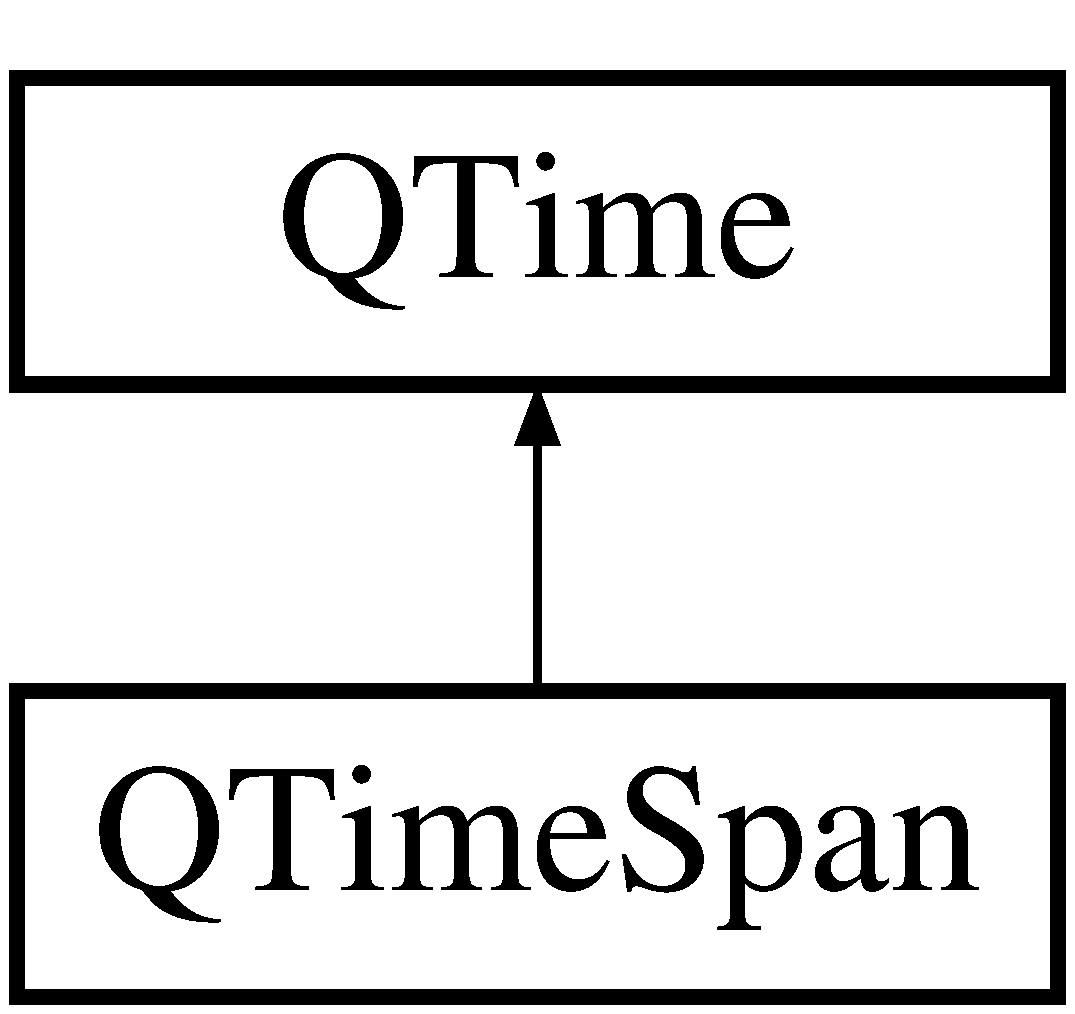
\includegraphics[height=2.000000cm]{class_q_time_span}
\end{center}
\end{figure}
\subsection*{Fonctions membres publiques}
\begin{DoxyCompactItemize}
\item 
\hypertarget{class_q_time_span_a8cd29696e67c41f49f5a240e9e78cabe}{}{\bfseries Q\+Time\+Span} (const Q\+Time \&horaire)\label{class_q_time_span_a8cd29696e67c41f49f5a240e9e78cabe}

\item 
\hypertarget{class_q_time_span_a00f65e986fe17b60dd36cd028c19ce0f}{}{\bfseries Q\+Time\+Span} (int h, int m, int s=0, int ms=0)\label{class_q_time_span_a00f65e986fe17b60dd36cd028c19ce0f}

\item 
\hyperlink{class_q_time_span}{Q\+Time\+Span} \hyperlink{class_q_time_span_af687464e1116164d0c32c4655b024560}{operator+} (const \hyperlink{class_q_time_span}{Q\+Time\+Span} \&d) const 
\item 
\hyperlink{class_q_time_span}{Q\+Time\+Span} \& \hyperlink{class_q_time_span_a038fd914f077796445c578374d066fe5}{operator+=} (const \hyperlink{class_q_time_span}{Q\+Time\+Span} \&d)
\item 
\hyperlink{class_q_time_span}{Q\+Time\+Span} \hyperlink{class_q_time_span_a2a68d770016787234f2d4b1fb6e05335}{operator-\/} (const \hyperlink{class_q_time_span}{Q\+Time\+Span} \&d) const 
\item 
\hyperlink{class_q_time_span}{Q\+Time\+Span} \& \hyperlink{class_q_time_span_a68657d22a32edb47bd04776162038031}{operator-\/=} (const \hyperlink{class_q_time_span}{Q\+Time\+Span} \&d)
\end{DoxyCompactItemize}


\subsection{Description détaillée}
Classe permettant de manipuler les temps/durées en implémentant l\textquotesingle{}addition et la soustraction manquantes à classe Q\+Time. 

\subsection{Documentation des fonctions membres}
\hypertarget{class_q_time_span_af687464e1116164d0c32c4655b024560}{}\index{Q\+Time\+Span@{Q\+Time\+Span}!operator+@{operator+}}
\index{operator+@{operator+}!Q\+Time\+Span@{Q\+Time\+Span}}
\subsubsection[{operator+}]{\setlength{\rightskip}{0pt plus 5cm}{\bf Q\+Time\+Span} Q\+Time\+Span\+::operator+ (
\begin{DoxyParamCaption}
\item[{const {\bf Q\+Time\+Span} \&}]{d}
\end{DoxyParamCaption}
) const}\label{class_q_time_span_af687464e1116164d0c32c4655b024560}
Opérateur d\textquotesingle{}addition permettant d\textquotesingle{}additionner deux \hyperlink{class_q_time_span}{Q\+Time\+Span} et leurs attributs respectifs. \hypertarget{class_q_time_span_a038fd914f077796445c578374d066fe5}{}\index{Q\+Time\+Span@{Q\+Time\+Span}!operator+=@{operator+=}}
\index{operator+=@{operator+=}!Q\+Time\+Span@{Q\+Time\+Span}}
\subsubsection[{operator+=}]{\setlength{\rightskip}{0pt plus 5cm}{\bf Q\+Time\+Span} \& Q\+Time\+Span\+::operator+= (
\begin{DoxyParamCaption}
\item[{const {\bf Q\+Time\+Span} \&}]{d}
\end{DoxyParamCaption}
)}\label{class_q_time_span_a038fd914f077796445c578374d066fe5}
Opérateur d\textquotesingle{}addition permettant d\textquotesingle{}additionner deux \hyperlink{class_q_time_span}{Q\+Time\+Span} et leurs attributs respectifs. \hypertarget{class_q_time_span_a2a68d770016787234f2d4b1fb6e05335}{}\index{Q\+Time\+Span@{Q\+Time\+Span}!operator-\/@{operator-\/}}
\index{operator-\/@{operator-\/}!Q\+Time\+Span@{Q\+Time\+Span}}
\subsubsection[{operator-\/}]{\setlength{\rightskip}{0pt plus 5cm}{\bf Q\+Time\+Span} Q\+Time\+Span\+::operator-\/ (
\begin{DoxyParamCaption}
\item[{const {\bf Q\+Time\+Span} \&}]{d}
\end{DoxyParamCaption}
) const}\label{class_q_time_span_a2a68d770016787234f2d4b1fb6e05335}
Opérateur de soustraction permettant de soustraire deux \hyperlink{class_q_time_span}{Q\+Time\+Span} et leurs attributs respectifs. \hypertarget{class_q_time_span_a68657d22a32edb47bd04776162038031}{}\index{Q\+Time\+Span@{Q\+Time\+Span}!operator-\/=@{operator-\/=}}
\index{operator-\/=@{operator-\/=}!Q\+Time\+Span@{Q\+Time\+Span}}
\subsubsection[{operator-\/=}]{\setlength{\rightskip}{0pt plus 5cm}{\bf Q\+Time\+Span} \& Q\+Time\+Span\+::operator-\/= (
\begin{DoxyParamCaption}
\item[{const {\bf Q\+Time\+Span} \&}]{d}
\end{DoxyParamCaption}
)}\label{class_q_time_span_a68657d22a32edb47bd04776162038031}
Opérateur de soustraction permettant de soustraire deux \hyperlink{class_q_time_span}{Q\+Time\+Span} et leurs attributs respectifs. 

La documentation de cette classe a été générée à partir des fichiers suivants \+:\begin{DoxyCompactItemize}
\item 
qtimespan.\+h\item 
qtimespan.\+cpp\end{DoxyCompactItemize}

\hypertarget{class_tache}{}\section{Référence de la classe Tache}
\label{class_tache}\index{Tache@{Tache}}


La classe \hyperlink{class_tache}{Tache} est virtuelle pure, seules ses classes filles\+: tâche unitaire et tâche composite peuvent être instanciées, par le \hyperlink{class_tache_manager}{Tache\+Manager}.  




{\ttfamily \#include $<$evenement.\+h$>$}

Graphe d\textquotesingle{}héritage de Tache\+:\begin{figure}[H]
\begin{center}
\leavevmode
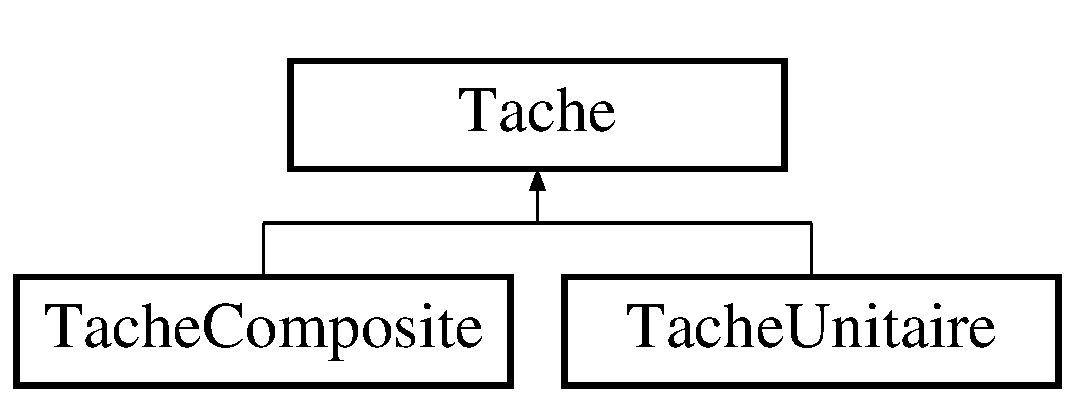
\includegraphics[height=2.000000cm]{class_tache}
\end{center}
\end{figure}
\subsection*{Fonctions membres publiques}
\begin{DoxyCompactItemize}
\item 
\hyperlink{class_projet}{Projet} $\ast$ \hyperlink{class_tache_ab625a7bde0e9ef9cbb8bb07696cdd985}{get\+Projet} () const 
\item 
vector$<$ \hyperlink{class_precedence}{Precedence} $\ast$ $>$ \hyperlink{class_tache_a663555dc2753ade57ceb7b3407e01fca}{get\+Precedences} () const 
\item 
const Q\+Date\+Time \& \hyperlink{class_tache_af01274a0f287d4598c611e65ff560509}{get\+Disponibilite} () const 
\item 
const Q\+Date\+Time \& \hyperlink{class_tache_a31bc22c34f6f3630192009245347da71}{get\+Echeance} () const 
\item 
const Q\+String \& \hyperlink{class_tache_a1f9ccf770c1873bbaa1c63aba11c198e}{get\+Titre} () const 
\item 
const Q\+String \& \hyperlink{class_tache_ab8354f8832fb8f1ed8e911c53f9ecb51}{get\+Id} () const 
\item 
void \hyperlink{class_tache_ab86e1a897f1da92bedad09af497a4076}{set\+Id} (const Q\+String \&i)
\item 
void \hyperlink{class_tache_afade5c5180edea94d258da777b2006df}{set\+Titre} (const Q\+String \&t)
\item 
void \hyperlink{class_tache_a3ee16d4ce77af8bae5ceea485d4fce79}{set\+Disponibilite} (const Q\+String \&d)
\item 
void \hyperlink{class_tache_a1d06b03ee9f2c60ef43ffb8fc7cacdba}{set\+Echeance} (const Q\+String \&e)
\item 
void \hyperlink{class_tache_ad48e1f420a9acdb88d05fab52ddcc402}{set\+Projet} (\hyperlink{class_projet}{Projet} \&p)
\item 
void \hyperlink{class_tache_aaceff1bb035b504fdcc06401515b66d8}{set\+Projet} (const Q\+String \&id)
\item 
\hyperlink{class_tache_composite}{Tache\+Composite} $\ast$ \hyperlink{class_tache_a69fe54e6a7551244a18101764256c3cd}{get\+Composite} () const 
\item 
virtual void \hyperlink{class_tache_a5f22769fadb598764c937d65a901946f}{set\+Disponibilite\+D\+T} (const Q\+Date\+Time \&d)
\item 
\hypertarget{class_tache_add128bd3a8b4832f4e6f52e0ee80e16b}{}virtual void \hyperlink{class_tache_add128bd3a8b4832f4e6f52e0ee80e16b}{set\+Echeance\+D\+T} (const Q\+Date\+Time \&e)\label{class_tache_add128bd3a8b4832f4e6f52e0ee80e16b}

\begin{DoxyCompactList}\small\item\em La méthode \hyperlink{class_tache_add128bd3a8b4832f4e6f52e0ee80e16b}{set\+Echeance\+D\+T()} met à jour la date d\textquotesingle{}écheance de la tâche avec la date passée en paramètre. \end{DoxyCompactList}\item 
virtual void \hyperlink{class_tache_aa56e1690299f9b6892d21e10df7768b0}{afficher} () const 
\item 
\hypertarget{class_tache_acde59bde54ea8be7c5cbdca0267e7092}{}virtual Q\+String {\bfseries who\+Am\+I} () const =0\label{class_tache_acde59bde54ea8be7c5cbdca0267e7092}

\end{DoxyCompactItemize}
\subsection*{Fonctions membres protégées}
\begin{DoxyCompactItemize}
\item 
\hypertarget{class_tache_a5323cf9614ab261150a163937261c8b6}{}{\bfseries Tache} (const Q\+String \&id, const Q\+String \&title, const Q\+Date\+Time \&dispo, const Q\+Date\+Time \&echeance)\label{class_tache_a5323cf9614ab261150a163937261c8b6}

\item 
\hypertarget{class_tache_af154eeeb0bcfa9f8364025260d5f70b6}{}{\bfseries Tache} (const \hyperlink{class_tache}{Tache} \&t)\label{class_tache_af154eeeb0bcfa9f8364025260d5f70b6}

\item 
\hypertarget{class_tache_a481a4c75b9908ff79ef9dc9b8e957b51}{}const \hyperlink{class_tache}{Tache} \& {\bfseries operator=} (const \hyperlink{class_tache}{Tache} \&t)\label{class_tache_a481a4c75b9908ff79ef9dc9b8e957b51}

\end{DoxyCompactItemize}
\subsection*{Attributs protégés}
\begin{DoxyCompactItemize}
\item 
\hypertarget{class_tache_ae22f26aa33762082872376475946acff}{}Q\+String {\bfseries identificateur}\label{class_tache_ae22f26aa33762082872376475946acff}

\item 
\hypertarget{class_tache_a1d3d20046c0c4cc8482f71bb555b79cf}{}Q\+String {\bfseries titre}\label{class_tache_a1d3d20046c0c4cc8482f71bb555b79cf}

\item 
\hypertarget{class_tache_ad4d89bbfb2bd93ecf00e790ab792799d}{}Q\+Date\+Time {\bfseries date\+\_\+echeance}\label{class_tache_ad4d89bbfb2bd93ecf00e790ab792799d}

\item 
\hypertarget{class_tache_a6a892b5554571cabd823b1dae1ab270d}{}Q\+Date\+Time {\bfseries date\+\_\+dispo}\label{class_tache_a6a892b5554571cabd823b1dae1ab270d}

\end{DoxyCompactItemize}
\subsection*{Amis}
\begin{DoxyCompactItemize}
\item 
\hypertarget{class_tache_a59876a285574eb2b160307049a269610}{}class {\bfseries Tache\+Manager}\label{class_tache_a59876a285574eb2b160307049a269610}

\item 
\hypertarget{class_tache_a46c1844e74be2532f86bf3a09ec141e7}{}class {\bfseries Manager$<$ Tache, Tache\+Manager $>$}\label{class_tache_a46c1844e74be2532f86bf3a09ec141e7}

\end{DoxyCompactItemize}


\subsection{Description détaillée}
La classe \hyperlink{class_tache}{Tache} est virtuelle pure, seules ses classes filles\+: tâche unitaire et tâche composite peuvent être instanciées, par le \hyperlink{class_tache_manager}{Tache\+Manager}. 

\subsection{Documentation des fonctions membres}
\hypertarget{class_tache_aa56e1690299f9b6892d21e10df7768b0}{}\index{Tache@{Tache}!afficher@{afficher}}
\index{afficher@{afficher}!Tache@{Tache}}
\subsubsection[{afficher}]{\setlength{\rightskip}{0pt plus 5cm}void Tache\+::afficher (
\begin{DoxyParamCaption}
{}
\end{DoxyParamCaption}
) const\hspace{0.3cm}{\ttfamily [virtual]}}\label{class_tache_aa56e1690299f9b6892d21e10df7768b0}
La méthode \hyperlink{class_tache_aa56e1690299f9b6892d21e10df7768b0}{afficher()} permet d\textquotesingle{}afficher en mode debug les attributs de la tâche.

Réimplémentée dans \hyperlink{class_tache_unitaire_a8f28f8372a319aaee49881487f530a60}{Tache\+Unitaire}.

\hypertarget{class_tache_a69fe54e6a7551244a18101764256c3cd}{}\index{Tache@{Tache}!get\+Composite@{get\+Composite}}
\index{get\+Composite@{get\+Composite}!Tache@{Tache}}
\subsubsection[{get\+Composite}]{\setlength{\rightskip}{0pt plus 5cm}{\bf Tache\+Composite} $\ast$ Tache\+::get\+Composite (
\begin{DoxyParamCaption}
{}
\end{DoxyParamCaption}
) const}\label{class_tache_a69fe54e6a7551244a18101764256c3cd}
La méthode \hyperlink{class_tache_a69fe54e6a7551244a18101764256c3cd}{get\+Composite()} renvoie un pointeur sur la tâche composite composé de la tâche. Si cette dernière ne compose pas de tâche composite, un pointeur null sera renvoyé.\hypertarget{class_tache_af01274a0f287d4598c611e65ff560509}{}\index{Tache@{Tache}!get\+Disponibilite@{get\+Disponibilite}}
\index{get\+Disponibilite@{get\+Disponibilite}!Tache@{Tache}}
\subsubsection[{get\+Disponibilite}]{\setlength{\rightskip}{0pt plus 5cm}const Q\+Date\+Time\& Tache\+::get\+Disponibilite (
\begin{DoxyParamCaption}
{}
\end{DoxyParamCaption}
) const\hspace{0.3cm}{\ttfamily [inline]}}\label{class_tache_af01274a0f287d4598c611e65ff560509}
La méthode \hyperlink{class_tache_af01274a0f287d4598c611e65ff560509}{get\+Disponibilite()} renvoie la date de disponibilité de la tâche. \hypertarget{class_tache_a31bc22c34f6f3630192009245347da71}{}\index{Tache@{Tache}!get\+Echeance@{get\+Echeance}}
\index{get\+Echeance@{get\+Echeance}!Tache@{Tache}}
\subsubsection[{get\+Echeance}]{\setlength{\rightskip}{0pt plus 5cm}const Q\+Date\+Time\& Tache\+::get\+Echeance (
\begin{DoxyParamCaption}
{}
\end{DoxyParamCaption}
) const\hspace{0.3cm}{\ttfamily [inline]}}\label{class_tache_a31bc22c34f6f3630192009245347da71}
La méthode \hyperlink{class_tache_a31bc22c34f6f3630192009245347da71}{get\+Echeance()} renvoie la date d\textquotesingle{}écheance de la tâche. \hypertarget{class_tache_ab8354f8832fb8f1ed8e911c53f9ecb51}{}\index{Tache@{Tache}!get\+Id@{get\+Id}}
\index{get\+Id@{get\+Id}!Tache@{Tache}}
\subsubsection[{get\+Id}]{\setlength{\rightskip}{0pt plus 5cm}const Q\+String\& Tache\+::get\+Id (
\begin{DoxyParamCaption}
{}
\end{DoxyParamCaption}
) const\hspace{0.3cm}{\ttfamily [inline]}}\label{class_tache_ab8354f8832fb8f1ed8e911c53f9ecb51}
La méthode \hyperlink{class_tache_ab8354f8832fb8f1ed8e911c53f9ecb51}{get\+Id()} renvoie l\textquotesingle{}identificateur de la tâche. \hypertarget{class_tache_a663555dc2753ade57ceb7b3407e01fca}{}\index{Tache@{Tache}!get\+Precedences@{get\+Precedences}}
\index{get\+Precedences@{get\+Precedences}!Tache@{Tache}}
\subsubsection[{get\+Precedences}]{\setlength{\rightskip}{0pt plus 5cm}vector$<$ {\bf Precedence} $\ast$ $>$ Tache\+::get\+Precedences (
\begin{DoxyParamCaption}
{}
\end{DoxyParamCaption}
) const}\label{class_tache_a663555dc2753ade57ceb7b3407e01fca}
La méthode \hyperlink{class_tache_a663555dc2753ade57ceb7b3407e01fca}{get\+Precedences()} renvoie un vecteur contenant les précédences de la tache.\hypertarget{class_tache_ab625a7bde0e9ef9cbb8bb07696cdd985}{}\index{Tache@{Tache}!get\+Projet@{get\+Projet}}
\index{get\+Projet@{get\+Projet}!Tache@{Tache}}
\subsubsection[{get\+Projet}]{\setlength{\rightskip}{0pt plus 5cm}{\bf Projet} $\ast$ Tache\+::get\+Projet (
\begin{DoxyParamCaption}
{}
\end{DoxyParamCaption}
) const}\label{class_tache_ab625a7bde0e9ef9cbb8bb07696cdd985}
La méthode \hyperlink{class_tache_ab625a7bde0e9ef9cbb8bb07696cdd985}{get\+Projet()} renvoie un pointeur sur le projet lié à la tâche. Si la tache n\textquotesingle{}est dans aucun projet, \hyperlink{class_tache_ab625a7bde0e9ef9cbb8bb07696cdd985}{get\+Projet()} renvoie un pointeur null.\hypertarget{class_tache_a1f9ccf770c1873bbaa1c63aba11c198e}{}\index{Tache@{Tache}!get\+Titre@{get\+Titre}}
\index{get\+Titre@{get\+Titre}!Tache@{Tache}}
\subsubsection[{get\+Titre}]{\setlength{\rightskip}{0pt plus 5cm}const Q\+String\& Tache\+::get\+Titre (
\begin{DoxyParamCaption}
{}
\end{DoxyParamCaption}
) const\hspace{0.3cm}{\ttfamily [inline]}}\label{class_tache_a1f9ccf770c1873bbaa1c63aba11c198e}
La méthode \hyperlink{class_tache_a1f9ccf770c1873bbaa1c63aba11c198e}{get\+Titre()} renvoie le titre de la tâche. \hypertarget{class_tache_a3ee16d4ce77af8bae5ceea485d4fce79}{}\index{Tache@{Tache}!set\+Disponibilite@{set\+Disponibilite}}
\index{set\+Disponibilite@{set\+Disponibilite}!Tache@{Tache}}
\subsubsection[{set\+Disponibilite}]{\setlength{\rightskip}{0pt plus 5cm}void Tache\+::set\+Disponibilite (
\begin{DoxyParamCaption}
\item[{const Q\+String \&}]{d}
\end{DoxyParamCaption}
)}\label{class_tache_a3ee16d4ce77af8bae5ceea485d4fce79}
La méthode \hyperlink{class_tache_a3ee16d4ce77af8bae5ceea485d4fce79}{set\+Disponibilite()} permet de modifier la date de disponibilite de la tâche.\hypertarget{class_tache_a5f22769fadb598764c937d65a901946f}{}\index{Tache@{Tache}!set\+Disponibilite\+D\+T@{set\+Disponibilite\+D\+T}}
\index{set\+Disponibilite\+D\+T@{set\+Disponibilite\+D\+T}!Tache@{Tache}}
\subsubsection[{set\+Disponibilite\+D\+T}]{\setlength{\rightskip}{0pt plus 5cm}virtual void Tache\+::set\+Disponibilite\+D\+T (
\begin{DoxyParamCaption}
\item[{const Q\+Date\+Time \&}]{d}
\end{DoxyParamCaption}
)\hspace{0.3cm}{\ttfamily [inline]}, {\ttfamily [virtual]}}\label{class_tache_a5f22769fadb598764c937d65a901946f}
La méthode \hyperlink{class_tache_a5f22769fadb598764c937d65a901946f}{set\+Disponibilite\+D\+T()} met à jour la date de disponibilite de la tâche avec la date passée en paramètre. 

Réimplémentée dans \hyperlink{class_tache_composite_a5032eaa67db81045f77dbf5446943261}{Tache\+Composite}.

\hypertarget{class_tache_a1d06b03ee9f2c60ef43ffb8fc7cacdba}{}\index{Tache@{Tache}!set\+Echeance@{set\+Echeance}}
\index{set\+Echeance@{set\+Echeance}!Tache@{Tache}}
\subsubsection[{set\+Echeance}]{\setlength{\rightskip}{0pt plus 5cm}void Tache\+::set\+Echeance (
\begin{DoxyParamCaption}
\item[{const Q\+String \&}]{e}
\end{DoxyParamCaption}
)}\label{class_tache_a1d06b03ee9f2c60ef43ffb8fc7cacdba}
La méthode \hyperlink{class_tache_a1d06b03ee9f2c60ef43ffb8fc7cacdba}{set\+Echeance()} permet de modifier la date d\textquotesingle{}écheance de la tâche.\hypertarget{class_tache_ab86e1a897f1da92bedad09af497a4076}{}\index{Tache@{Tache}!set\+Id@{set\+Id}}
\index{set\+Id@{set\+Id}!Tache@{Tache}}
\subsubsection[{set\+Id}]{\setlength{\rightskip}{0pt plus 5cm}void Tache\+::set\+Id (
\begin{DoxyParamCaption}
\item[{const Q\+String \&}]{i}
\end{DoxyParamCaption}
)\hspace{0.3cm}{\ttfamily [inline]}}\label{class_tache_ab86e1a897f1da92bedad09af497a4076}
La méthode \hyperlink{class_tache_ab86e1a897f1da92bedad09af497a4076}{set\+Id()} met à jour l\textquotesingle{}identificateur de la tâche avec la chaine passée en paramètre. \hypertarget{class_tache_ad48e1f420a9acdb88d05fab52ddcc402}{}\index{Tache@{Tache}!set\+Projet@{set\+Projet}}
\index{set\+Projet@{set\+Projet}!Tache@{Tache}}
\subsubsection[{set\+Projet}]{\setlength{\rightskip}{0pt plus 5cm}void Tache\+::set\+Projet (
\begin{DoxyParamCaption}
\item[{{\bf Projet} \&}]{p}
\end{DoxyParamCaption}
)}\label{class_tache_ad48e1f420a9acdb88d05fab52ddcc402}
La méthode set\+Projet permet de lier une tâche à un projet. Si cette dernière est déjà liée, cette liaison sera supprimée puis remplacée.\hypertarget{class_tache_aaceff1bb035b504fdcc06401515b66d8}{}\index{Tache@{Tache}!set\+Projet@{set\+Projet}}
\index{set\+Projet@{set\+Projet}!Tache@{Tache}}
\subsubsection[{set\+Projet}]{\setlength{\rightskip}{0pt plus 5cm}void Tache\+::set\+Projet (
\begin{DoxyParamCaption}
\item[{const Q\+String \&}]{id}
\end{DoxyParamCaption}
)}\label{class_tache_aaceff1bb035b504fdcc06401515b66d8}
Voir \hyperlink{class_tache_ad48e1f420a9acdb88d05fab52ddcc402}{set\+Projet(\+Projet\& P)}.\hypertarget{class_tache_afade5c5180edea94d258da777b2006df}{}\index{Tache@{Tache}!set\+Titre@{set\+Titre}}
\index{set\+Titre@{set\+Titre}!Tache@{Tache}}
\subsubsection[{set\+Titre}]{\setlength{\rightskip}{0pt plus 5cm}void Tache\+::set\+Titre (
\begin{DoxyParamCaption}
\item[{const Q\+String \&}]{t}
\end{DoxyParamCaption}
)\hspace{0.3cm}{\ttfamily [inline]}}\label{class_tache_afade5c5180edea94d258da777b2006df}
La méthode \hyperlink{class_tache_afade5c5180edea94d258da777b2006df}{set\+Titre()} met à jour le titre de la tâche avec la chaine passée en paramètre. 

La documentation de cette classe a été générée à partir des fichiers suivants \+:\begin{DoxyCompactItemize}
\item 
evenement.\+h\item 
evenement.\+cpp\end{DoxyCompactItemize}

\hypertarget{class_tache_composite}{}\section{Référence de la classe Tache\+Composite}
\label{class_tache_composite}\index{Tache\+Composite@{Tache\+Composite}}


Une \hyperlink{class_tache_composite}{Tache\+Composite} est une tâche non-\/programmable composée d\textquotesingle{}autres tâches, pouvant être unitaires ou composites. Elle ne peut être instanciée que par le biais \hyperlink{class_tache_manager}{Tache\+Manager}.  




{\ttfamily \#include $<$evenement.\+h$>$}

Graphe d\textquotesingle{}héritage de Tache\+Composite\+:\begin{figure}[H]
\begin{center}
\leavevmode
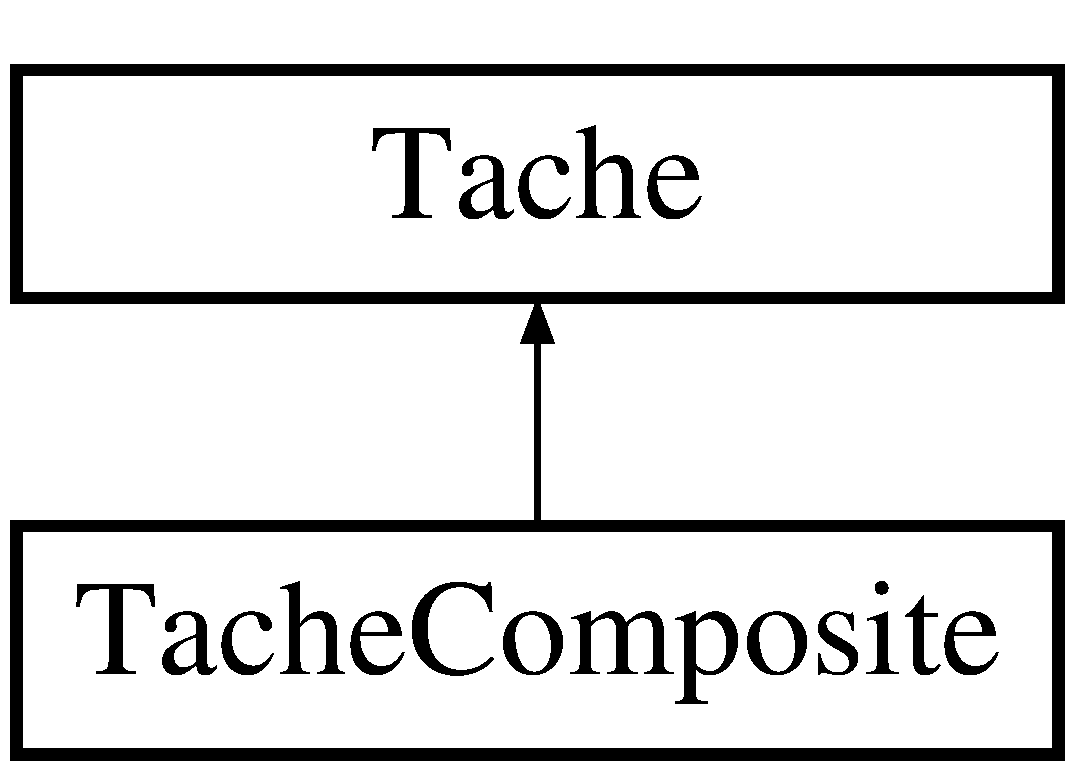
\includegraphics[height=2.000000cm]{class_tache_composite}
\end{center}
\end{figure}
\subsection*{Classes}
\begin{DoxyCompactItemize}
\item 
class \hyperlink{class_tache_composite_1_1const__iterator}{const\+\_\+iterator}
\item 
class \hyperlink{class_tache_composite_1_1iterator}{iterator}
\end{DoxyCompactItemize}
\subsection*{Fonctions membres publiques}
\begin{DoxyCompactItemize}
\item 
size\+\_\+t \hyperlink{class_tache_composite_af1ba658a78e4e6f1080b9c000eba4201}{get\+Size} ()
\item 
\hyperlink{class_tache_composite_1_1iterator}{iterator} \hyperlink{class_tache_composite_a0ddf3aa66c03324530c1edae9e51d97b}{begin} ()
\item 
\hyperlink{class_tache_composite_1_1iterator}{iterator} \hyperlink{class_tache_composite_a19085d7f01e368efab4ec40f63a04117}{end} ()
\item 
\hyperlink{class_tache_composite_1_1const__iterator}{const\+\_\+iterator} \hyperlink{class_tache_composite_a08938304455ed31cc3219677787d376e}{begin} () const 
\item 
\hyperlink{class_tache_composite_1_1const__iterator}{const\+\_\+iterator} \hyperlink{class_tache_composite_adc3b95cd5e0da1d570535356a7e18ecb}{end} () const 
\item 
bool \hyperlink{class_tache_composite_afbbffa746a783c2f5475bd2746bdc318}{is\+Composable} (const \hyperlink{class_tache}{Tache} \&t) const 
\item 
void \hyperlink{class_tache_composite_a560d35db6e3c5c0961fcc7224f65765d}{push\+\_\+back} (\hyperlink{class_tache}{Tache} \&t)
\item 
void \hyperlink{class_tache_composite_a8f6db68650bf23621041520216dd1a2a}{pop\+\_\+back} ()
\item 
\hyperlink{class_tache_composite_1_1iterator}{iterator} \hyperlink{class_tache_composite_af456d1818e34d4e7a91c624a28de2f78}{erase} (\hyperlink{class_tache_composite_1_1iterator}{iterator} position)
\item 
void \hyperlink{class_tache_composite_a5032eaa67db81045f77dbf5446943261}{set\+Disponibilite\+D\+T} (const Q\+Date\+Time \&dispo) override
\item 
void \hyperlink{class_tache_composite_a286829ee84d887a7416318a07fb72a2e}{set\+Echeance\+D\+T} (const Q\+Date\+Time \&echeance) override
\begin{DoxyCompactList}\small\item\em La méthode \hyperlink{class_tache_composite_a286829ee84d887a7416318a07fb72a2e}{set\+Echeance\+D\+T()} met à jour la date d\textquotesingle{}écheance de la tâche avec la date passée en paramètre. \end{DoxyCompactList}\item 
void \hyperlink{class_tache_composite_a784957f6b9a7b7ccb0105e8e73104567}{afficher} ()
\item 
Q\+String \hyperlink{class_tache_composite_ac49737e53296e809078d099de5525973}{who\+Am\+I} () const 
\end{DoxyCompactItemize}
\subsection*{Amis}
\begin{DoxyCompactItemize}
\item 
\hypertarget{class_tache_composite_a59876a285574eb2b160307049a269610}{}class {\bfseries Tache\+Manager}\label{class_tache_composite_a59876a285574eb2b160307049a269610}

\item 
\hypertarget{class_tache_composite_a46c1844e74be2532f86bf3a09ec141e7}{}class {\bfseries Manager$<$ Tache, Tache\+Manager $>$}\label{class_tache_composite_a46c1844e74be2532f86bf3a09ec141e7}

\end{DoxyCompactItemize}
\subsection*{Membres hérités additionnels}


\subsection{Description détaillée}
Une \hyperlink{class_tache_composite}{Tache\+Composite} est une tâche non-\/programmable composée d\textquotesingle{}autres tâches, pouvant être unitaires ou composites. Elle ne peut être instanciée que par le biais \hyperlink{class_tache_manager}{Tache\+Manager}. 

\subsection{Documentation des fonctions membres}
\hypertarget{class_tache_composite_a784957f6b9a7b7ccb0105e8e73104567}{}\index{Tache\+Composite@{Tache\+Composite}!afficher@{afficher}}
\index{afficher@{afficher}!Tache\+Composite@{Tache\+Composite}}
\subsubsection[{afficher}]{\setlength{\rightskip}{0pt plus 5cm}void Tache\+Composite\+::afficher (
\begin{DoxyParamCaption}
{}
\end{DoxyParamCaption}
)}\label{class_tache_composite_a784957f6b9a7b7ccb0105e8e73104567}
La méthode \hyperlink{class_tache_composite_a784957f6b9a7b7ccb0105e8e73104567}{afficher()} permet d\textquotesingle{}afficher en mode debug les attributs et tâches composantes de la tâche composite.\hypertarget{class_tache_composite_a0ddf3aa66c03324530c1edae9e51d97b}{}\index{Tache\+Composite@{Tache\+Composite}!begin@{begin}}
\index{begin@{begin}!Tache\+Composite@{Tache\+Composite}}
\subsubsection[{begin}]{\setlength{\rightskip}{0pt plus 5cm}{\bf iterator} Tache\+Composite\+::begin (
\begin{DoxyParamCaption}
{}
\end{DoxyParamCaption}
)\hspace{0.3cm}{\ttfamily [inline]}}\label{class_tache_composite_a0ddf3aa66c03324530c1edae9e51d97b}
Renvoie un iterator sur la première tâche composante. \hypertarget{class_tache_composite_a08938304455ed31cc3219677787d376e}{}\index{Tache\+Composite@{Tache\+Composite}!begin@{begin}}
\index{begin@{begin}!Tache\+Composite@{Tache\+Composite}}
\subsubsection[{begin}]{\setlength{\rightskip}{0pt plus 5cm}{\bf const\+\_\+iterator} Tache\+Composite\+::begin (
\begin{DoxyParamCaption}
{}
\end{DoxyParamCaption}
) const\hspace{0.3cm}{\ttfamily [inline]}}\label{class_tache_composite_a08938304455ed31cc3219677787d376e}
Renvoie un \hyperlink{class_tache_composite_1_1const__iterator}{const\+\_\+iterator} sur la première tâche composante \hypertarget{class_tache_composite_a19085d7f01e368efab4ec40f63a04117}{}\index{Tache\+Composite@{Tache\+Composite}!end@{end}}
\index{end@{end}!Tache\+Composite@{Tache\+Composite}}
\subsubsection[{end}]{\setlength{\rightskip}{0pt plus 5cm}{\bf iterator} Tache\+Composite\+::end (
\begin{DoxyParamCaption}
{}
\end{DoxyParamCaption}
)\hspace{0.3cm}{\ttfamily [inline]}}\label{class_tache_composite_a19085d7f01e368efab4ec40f63a04117}
Renvoie un iterator sur la fin du tableau de tâches composantes. \hypertarget{class_tache_composite_adc3b95cd5e0da1d570535356a7e18ecb}{}\index{Tache\+Composite@{Tache\+Composite}!end@{end}}
\index{end@{end}!Tache\+Composite@{Tache\+Composite}}
\subsubsection[{end}]{\setlength{\rightskip}{0pt plus 5cm}{\bf const\+\_\+iterator} Tache\+Composite\+::end (
\begin{DoxyParamCaption}
{}
\end{DoxyParamCaption}
) const\hspace{0.3cm}{\ttfamily [inline]}}\label{class_tache_composite_adc3b95cd5e0da1d570535356a7e18ecb}
Renvoie un \hyperlink{class_tache_composite_1_1const__iterator}{const\+\_\+iterator} sur la fin du tableau de tâches composantes. \hypertarget{class_tache_composite_af456d1818e34d4e7a91c624a28de2f78}{}\index{Tache\+Composite@{Tache\+Composite}!erase@{erase}}
\index{erase@{erase}!Tache\+Composite@{Tache\+Composite}}
\subsubsection[{erase}]{\setlength{\rightskip}{0pt plus 5cm}{\bf iterator} Tache\+Composite\+::erase (
\begin{DoxyParamCaption}
\item[{{\bf iterator}}]{position}
\end{DoxyParamCaption}
)\hspace{0.3cm}{\ttfamily [inline]}}\label{class_tache_composite_af456d1818e34d4e7a91c624a28de2f78}
Supprime le pointeur de tâche composante pointée par l\textquotesingle{}iterator \hypertarget{class_tache_composite_af1ba658a78e4e6f1080b9c000eba4201}{}\index{Tache\+Composite@{Tache\+Composite}!get\+Size@{get\+Size}}
\index{get\+Size@{get\+Size}!Tache\+Composite@{Tache\+Composite}}
\subsubsection[{get\+Size}]{\setlength{\rightskip}{0pt plus 5cm}size\+\_\+t Tache\+Composite\+::get\+Size (
\begin{DoxyParamCaption}
{}
\end{DoxyParamCaption}
)\hspace{0.3cm}{\ttfamily [inline]}}\label{class_tache_composite_af1ba658a78e4e6f1080b9c000eba4201}
Renvoie le nombre de taches composantes. \hypertarget{class_tache_composite_afbbffa746a783c2f5475bd2746bdc318}{}\index{Tache\+Composite@{Tache\+Composite}!is\+Composable@{is\+Composable}}
\index{is\+Composable@{is\+Composable}!Tache\+Composite@{Tache\+Composite}}
\subsubsection[{is\+Composable}]{\setlength{\rightskip}{0pt plus 5cm}bool Tache\+Composite\+::is\+Composable (
\begin{DoxyParamCaption}
\item[{const {\bf Tache} \&}]{t}
\end{DoxyParamCaption}
) const}\label{class_tache_composite_afbbffa746a783c2f5475bd2746bdc318}
La méthode \hyperlink{class_tache_composite_afbbffa746a783c2f5475bd2746bdc318}{is\+Composable()} renvoie true si la tâche en paramètre peut être inclue dans la tâche composite.\hypertarget{class_tache_composite_a8f6db68650bf23621041520216dd1a2a}{}\index{Tache\+Composite@{Tache\+Composite}!pop\+\_\+back@{pop\+\_\+back}}
\index{pop\+\_\+back@{pop\+\_\+back}!Tache\+Composite@{Tache\+Composite}}
\subsubsection[{pop\+\_\+back}]{\setlength{\rightskip}{0pt plus 5cm}void Tache\+Composite\+::pop\+\_\+back (
\begin{DoxyParamCaption}
{}
\end{DoxyParamCaption}
)\hspace{0.3cm}{\ttfamily [inline]}}\label{class_tache_composite_a8f6db68650bf23621041520216dd1a2a}
Supprime le pointeur vers la première tâche composante. \hypertarget{class_tache_composite_a560d35db6e3c5c0961fcc7224f65765d}{}\index{Tache\+Composite@{Tache\+Composite}!push\+\_\+back@{push\+\_\+back}}
\index{push\+\_\+back@{push\+\_\+back}!Tache\+Composite@{Tache\+Composite}}
\subsubsection[{push\+\_\+back}]{\setlength{\rightskip}{0pt plus 5cm}void Tache\+Composite\+::push\+\_\+back (
\begin{DoxyParamCaption}
\item[{{\bf Tache} \&}]{t}
\end{DoxyParamCaption}
)}\label{class_tache_composite_a560d35db6e3c5c0961fcc7224f65765d}
La méthode \hyperlink{class_tache_composite_a560d35db6e3c5c0961fcc7224f65765d}{push\+\_\+back()} vérifie si la tâche en paramètre peut être inclue dans la tâche composite. Si oui, elle ajoute cette tâche dans cette dernière. \hypertarget{class_tache_composite_a5032eaa67db81045f77dbf5446943261}{}\index{Tache\+Composite@{Tache\+Composite}!set\+Disponibilite\+D\+T@{set\+Disponibilite\+D\+T}}
\index{set\+Disponibilite\+D\+T@{set\+Disponibilite\+D\+T}!Tache\+Composite@{Tache\+Composite}}
\subsubsection[{set\+Disponibilite\+D\+T}]{\setlength{\rightskip}{0pt plus 5cm}void Tache\+Composite\+::set\+Disponibilite\+D\+T (
\begin{DoxyParamCaption}
\item[{const Q\+Date\+Time \&}]{dispo}
\end{DoxyParamCaption}
)\hspace{0.3cm}{\ttfamily [override]}, {\ttfamily [virtual]}}\label{class_tache_composite_a5032eaa67db81045f77dbf5446943261}
La méthode \hyperlink{class_tache_composite_a5032eaa67db81045f77dbf5446943261}{set\+Disponibilite\+D\+T()} permet de modifier la date de disponibilité de la tâche composite.

Réimplémentée à partir de \hyperlink{class_tache_a5f22769fadb598764c937d65a901946f}{Tache}.

\hypertarget{class_tache_composite_a286829ee84d887a7416318a07fb72a2e}{}\index{Tache\+Composite@{Tache\+Composite}!set\+Echeance\+D\+T@{set\+Echeance\+D\+T}}
\index{set\+Echeance\+D\+T@{set\+Echeance\+D\+T}!Tache\+Composite@{Tache\+Composite}}
\subsubsection[{set\+Echeance\+D\+T}]{\setlength{\rightskip}{0pt plus 5cm}void Tache\+Composite\+::set\+Echeance\+D\+T (
\begin{DoxyParamCaption}
\item[{const Q\+Date\+Time \&}]{e}
\end{DoxyParamCaption}
)\hspace{0.3cm}{\ttfamily [override]}, {\ttfamily [virtual]}}\label{class_tache_composite_a286829ee84d887a7416318a07fb72a2e}


La méthode \hyperlink{class_tache_composite_a286829ee84d887a7416318a07fb72a2e}{set\+Echeance\+D\+T()} met à jour la date d\textquotesingle{}écheance de la tâche avec la date passée en paramètre. 

La méthode \hyperlink{class_tache_composite_a5032eaa67db81045f77dbf5446943261}{set\+Disponibilite\+D\+T()} permet de modifier la date d\textquotesingle{}échéance de la tâche composite.

Réimplémentée à partir de \hyperlink{class_tache_add128bd3a8b4832f4e6f52e0ee80e16b}{Tache}.

\hypertarget{class_tache_composite_ac49737e53296e809078d099de5525973}{}\index{Tache\+Composite@{Tache\+Composite}!who\+Am\+I@{who\+Am\+I}}
\index{who\+Am\+I@{who\+Am\+I}!Tache\+Composite@{Tache\+Composite}}
\subsubsection[{who\+Am\+I}]{\setlength{\rightskip}{0pt plus 5cm}Q\+String Tache\+Composite\+::who\+Am\+I (
\begin{DoxyParamCaption}
{}
\end{DoxyParamCaption}
) const\hspace{0.3cm}{\ttfamily [inline]}, {\ttfamily [virtual]}}\label{class_tache_composite_ac49737e53296e809078d099de5525973}
Renvoie le type de tâche, ici \char`\"{}tache\+\_\+composite\char`\"{} 

Implémente \hyperlink{class_tache}{Tache}.



La documentation de cette classe a été générée à partir des fichiers suivants \+:\begin{DoxyCompactItemize}
\item 
evenement.\+h\item 
evenement.\+cpp\end{DoxyCompactItemize}

\hypertarget{classtache_editeur}{}\section{Référence de la classe tache\+Editeur}
\label{classtache_editeur}\index{tache\+Editeur@{tache\+Editeur}}


Fenêtre d\textquotesingle{}ajout et de modification de \hyperlink{class_tache_unitaire}{Tache\+Unitaire}.  




{\ttfamily \#include $<$tacheediteur.\+h$>$}

Graphe d\textquotesingle{}héritage de tache\+Editeur\+:\begin{figure}[H]
\begin{center}
\leavevmode
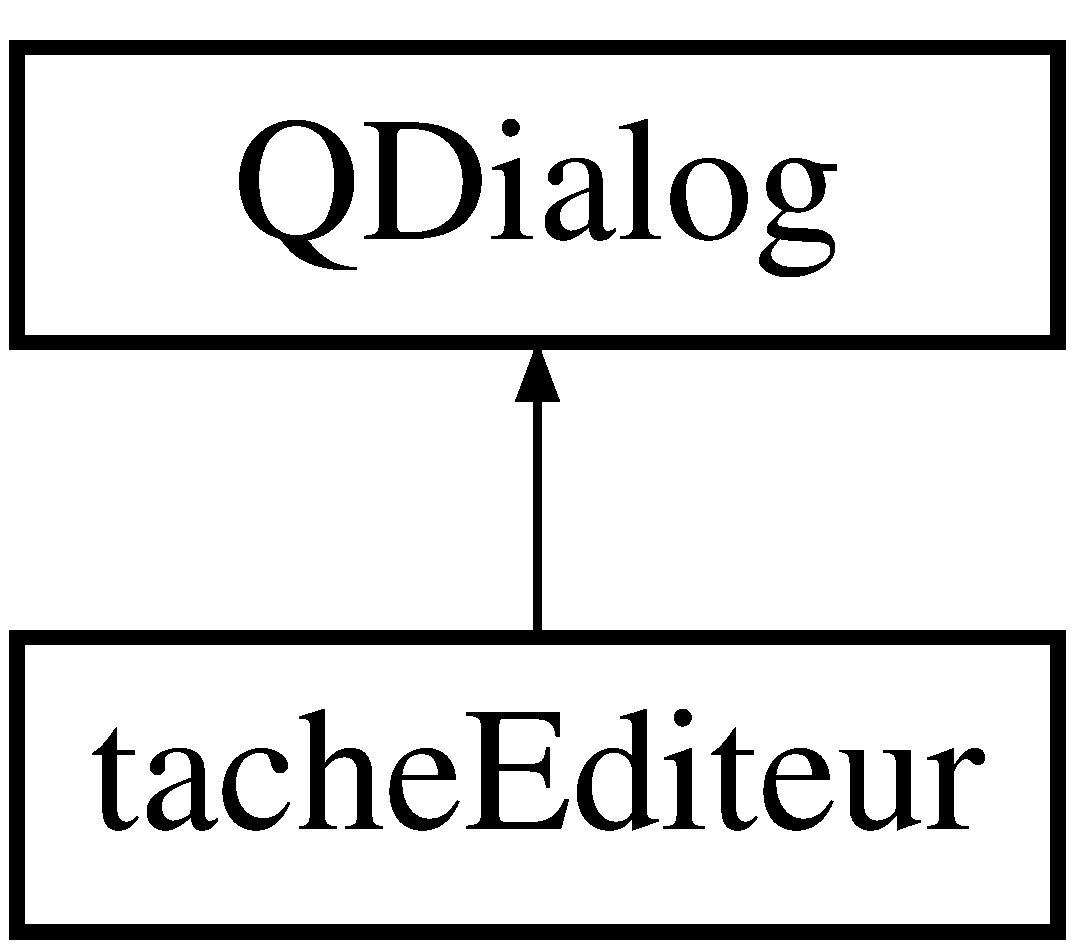
\includegraphics[height=2.000000cm]{classtache_editeur}
\end{center}
\end{figure}
\subsection*{Connecteurs publics}
\begin{DoxyCompactItemize}
\item 
\hypertarget{classtache_editeur_ab16a9e76ba7ef80478ff6eaf2e12c438}{}void {\bfseries sauver} ()\label{classtache_editeur_ab16a9e76ba7ef80478ff6eaf2e12c438}

\end{DoxyCompactItemize}
\subsection*{Fonctions membres publiques}
\begin{DoxyCompactItemize}
\item 
\hypertarget{classtache_editeur_ab1a1804a424319598c250665c34b4655}{}{\bfseries tache\+Editeur} (\hyperlink{class_tache_unitaire}{Tache\+Unitaire} $\ast$tache\+To\+Edit=0, Q\+Widget $\ast$parent=0)\label{classtache_editeur_ab1a1804a424319598c250665c34b4655}

\end{DoxyCompactItemize}


\subsection{Description détaillée}
Fenêtre d\textquotesingle{}ajout et de modification de \hyperlink{class_tache_unitaire}{Tache\+Unitaire}. 

La documentation de cette classe a été générée à partir des fichiers suivants \+:\begin{DoxyCompactItemize}
\item 
G\+U\+I/tacheediteur.\+h\item 
G\+U\+I/tacheediteur.\+cpp\end{DoxyCompactItemize}

\hypertarget{class_tache_manager}{}\section{Référence de la classe Tache\+Manager}
\label{class_tache_manager}\index{Tache\+Manager@{Tache\+Manager}}


La classe \hyperlink{class_tache_manager}{Tache\+Manager} est un \hyperlink{class_manager}{Manager} qui gère les items de type \hyperlink{class_tache}{Tache}. Elle ne peut être instanciée à cause du singleton mis en place dans sa classe mère. Elle peut toutefois être récupérée dans une référence ou un pointeur à l\textquotesingle{}aide la méthode mère\+: \hyperlink{class_manager_a8372e4f1e14f3605a57d839b152325ed}{get\+Instance()}.  




{\ttfamily \#include $<$manager.\+h$>$}

Graphe d\textquotesingle{}héritage de Tache\+Manager\+:\begin{figure}[H]
\begin{center}
\leavevmode
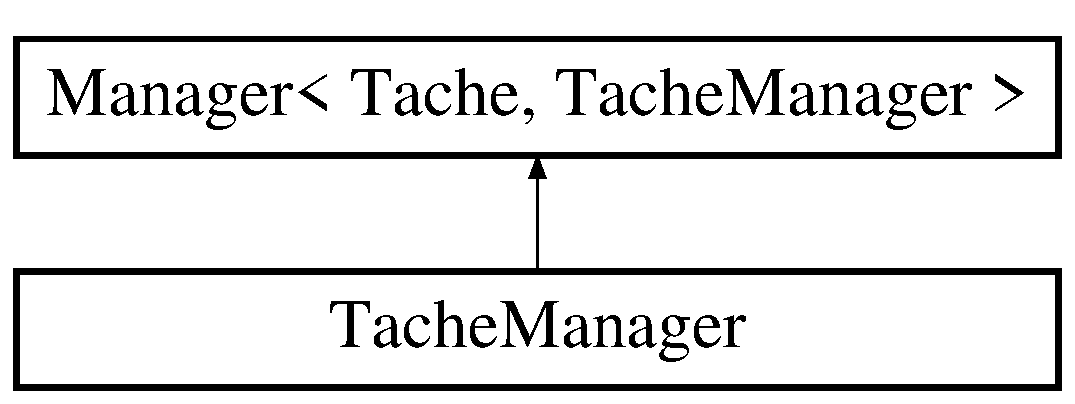
\includegraphics[height=2.000000cm]{class_tache_manager}
\end{center}
\end{figure}
\subsection*{Fonctions membres publiques}
\begin{DoxyCompactItemize}
\item 
\hyperlink{class_tache_unitaire}{Tache\+Unitaire} \& \hyperlink{class_tache_manager_aa9a015186cb6f439cc035a451d49ee90}{ajouter\+Tache\+Unitaire} (const Q\+String \&id, const Q\+String \&titre, const Q\+String \&duree, bool preemptive, const Q\+String \&dispo, const Q\+String \&echeance)
\item 
\hyperlink{class_tache_unitaire}{Tache\+Unitaire} \& \hyperlink{class_tache_manager_ab15a1f68d9e0c82d01d4751c954ddbf4}{ajouter\+Tache\+Unitaire} (const Q\+String \&id, const Q\+String \&titre, const \hyperlink{class_q_time_span}{Q\+Time\+Span} \&duree, bool preemptive, const Q\+Date\+Time \&dispo, const Q\+Date\+Time \&echeance)
\item 
\hyperlink{class_tache_composite}{Tache\+Composite} \& \hyperlink{class_tache_manager_aa8ab42b1e37f0a4965d836dd0ce22068}{ajouter\+Tache\+Composite} (const Q\+String \&id, const Q\+String \&titre, const Q\+String \&dispo, const Q\+String \&echeance, vector$<$ \hyperlink{class_tache}{Tache} $\ast$ $>$ liste=vector$<$ \hyperlink{class_tache}{Tache} $\ast$ $>$())
\item 
\hyperlink{class_tache_composite}{Tache\+Composite} \& \hyperlink{class_tache_manager_a27341ce34b6acd764275307e4d2eeeff}{ajouter\+Tache\+Composite} (const Q\+String \&id, const Q\+String \&titre, const Q\+Date\+Time \&dispo, const Q\+Date\+Time \&echeance, vector$<$ \hyperlink{class_tache}{Tache} $\ast$ $>$ liste=vector$<$ \hyperlink{class_tache}{Tache} $\ast$ $>$())
\end{DoxyCompactItemize}
\subsection*{Membres hérités additionnels}


\subsection{Description détaillée}
La classe \hyperlink{class_tache_manager}{Tache\+Manager} est un \hyperlink{class_manager}{Manager} qui gère les items de type \hyperlink{class_tache}{Tache}. Elle ne peut être instanciée à cause du singleton mis en place dans sa classe mère. Elle peut toutefois être récupérée dans une référence ou un pointeur à l\textquotesingle{}aide la méthode mère\+: \hyperlink{class_manager_a8372e4f1e14f3605a57d839b152325ed}{get\+Instance()}. 

\subsection{Documentation des fonctions membres}
\hypertarget{class_tache_manager_aa8ab42b1e37f0a4965d836dd0ce22068}{}\index{Tache\+Manager@{Tache\+Manager}!ajouter\+Tache\+Composite@{ajouter\+Tache\+Composite}}
\index{ajouter\+Tache\+Composite@{ajouter\+Tache\+Composite}!Tache\+Manager@{Tache\+Manager}}
\subsubsection[{ajouter\+Tache\+Composite}]{\setlength{\rightskip}{0pt plus 5cm}{\bf Tache\+Composite} \& Tache\+Manager\+::ajouter\+Tache\+Composite (
\begin{DoxyParamCaption}
\item[{const Q\+String \&}]{id, }
\item[{const Q\+String \&}]{titre, }
\item[{const Q\+String \&}]{dispo, }
\item[{const Q\+String \&}]{echeance, }
\item[{vector$<$ {\bf Tache} $\ast$ $>$}]{liste = {\ttfamily vector$<${\bf Tache}$\ast$$>$()}}
\end{DoxyParamCaption}
)}\label{class_tache_manager_aa8ab42b1e37f0a4965d836dd0ce22068}
Créer une tâche composite en vérifiant les attributs passés en paramètre, les contraintes de disponibilité, d\textquotesingle{}écheance, de précédence, mais également les contraintes liées aux tâches compostantes. Puis l\textquotesingle{}ajoute au vecteur et renvoie sa référence. \hypertarget{class_tache_manager_a27341ce34b6acd764275307e4d2eeeff}{}\index{Tache\+Manager@{Tache\+Manager}!ajouter\+Tache\+Composite@{ajouter\+Tache\+Composite}}
\index{ajouter\+Tache\+Composite@{ajouter\+Tache\+Composite}!Tache\+Manager@{Tache\+Manager}}
\subsubsection[{ajouter\+Tache\+Composite}]{\setlength{\rightskip}{0pt plus 5cm}{\bf Tache\+Composite} \& Tache\+Manager\+::ajouter\+Tache\+Composite (
\begin{DoxyParamCaption}
\item[{const Q\+String \&}]{id, }
\item[{const Q\+String \&}]{titre, }
\item[{const Q\+Date\+Time \&}]{dispo, }
\item[{const Q\+Date\+Time \&}]{echeance, }
\item[{vector$<$ {\bf Tache} $\ast$ $>$}]{liste = {\ttfamily vector$<${\bf Tache}$\ast$$>$()}}
\end{DoxyParamCaption}
)}\label{class_tache_manager_a27341ce34b6acd764275307e4d2eeeff}
Créer une tâche composite en vérifiant les attributs passés en paramètre, les contraintes de disponibilité, d\textquotesingle{}écheance, de précédence, mais également les contraintes liées aux tâches compostantes. Puis l\textquotesingle{}ajoute au vecteur et renvoie sa référence. \hypertarget{class_tache_manager_aa9a015186cb6f439cc035a451d49ee90}{}\index{Tache\+Manager@{Tache\+Manager}!ajouter\+Tache\+Unitaire@{ajouter\+Tache\+Unitaire}}
\index{ajouter\+Tache\+Unitaire@{ajouter\+Tache\+Unitaire}!Tache\+Manager@{Tache\+Manager}}
\subsubsection[{ajouter\+Tache\+Unitaire}]{\setlength{\rightskip}{0pt plus 5cm}{\bf Tache\+Unitaire} \& Tache\+Manager\+::ajouter\+Tache\+Unitaire (
\begin{DoxyParamCaption}
\item[{const Q\+String \&}]{id, }
\item[{const Q\+String \&}]{titre, }
\item[{const Q\+String \&}]{duree, }
\item[{bool}]{preemptive, }
\item[{const Q\+String \&}]{dispo, }
\item[{const Q\+String \&}]{echeance}
\end{DoxyParamCaption}
)}\label{class_tache_manager_aa9a015186cb6f439cc035a451d49ee90}
Créer une tâche unitaire, l\textquotesingle{}ajoute au vecteur et renvoie sa référence. \hypertarget{class_tache_manager_ab15a1f68d9e0c82d01d4751c954ddbf4}{}\index{Tache\+Manager@{Tache\+Manager}!ajouter\+Tache\+Unitaire@{ajouter\+Tache\+Unitaire}}
\index{ajouter\+Tache\+Unitaire@{ajouter\+Tache\+Unitaire}!Tache\+Manager@{Tache\+Manager}}
\subsubsection[{ajouter\+Tache\+Unitaire}]{\setlength{\rightskip}{0pt plus 5cm}{\bf Tache\+Unitaire} \& Tache\+Manager\+::ajouter\+Tache\+Unitaire (
\begin{DoxyParamCaption}
\item[{const Q\+String \&}]{id, }
\item[{const Q\+String \&}]{titre, }
\item[{const {\bf Q\+Time\+Span} \&}]{duree, }
\item[{bool}]{preemptive, }
\item[{const Q\+Date\+Time \&}]{dispo, }
\item[{const Q\+Date\+Time \&}]{echeance}
\end{DoxyParamCaption}
)}\label{class_tache_manager_ab15a1f68d9e0c82d01d4751c954ddbf4}
Créer une tâche unitaire en vérifiant les attributs passés en paramètre, les contraintes de disponibilité, d\textquotesingle{}écheance, de précédence, puis l\textquotesingle{}ajoute au vecteur et renvoie sa référence. 

La documentation de cette classe a été générée à partir des fichiers suivants \+:\begin{DoxyCompactItemize}
\item 
manager.\+h\item 
manager.\+cpp\end{DoxyCompactItemize}

\hypertarget{class_tache_unitaire}{}\section{Référence de la classe Tache\+Unitaire}
\label{class_tache_unitaire}\index{Tache\+Unitaire@{Tache\+Unitaire}}


Une \hyperlink{class_tache_unitaire}{Tache\+Unitaire} est une tâche programmable et composable. Elle ne peut être instanciée que par le biais du \hyperlink{class_tache_manager}{Tache\+Manager}.  




{\ttfamily \#include $<$evenement.\+h$>$}

Graphe d\textquotesingle{}héritage de Tache\+Unitaire\+:\begin{figure}[H]
\begin{center}
\leavevmode
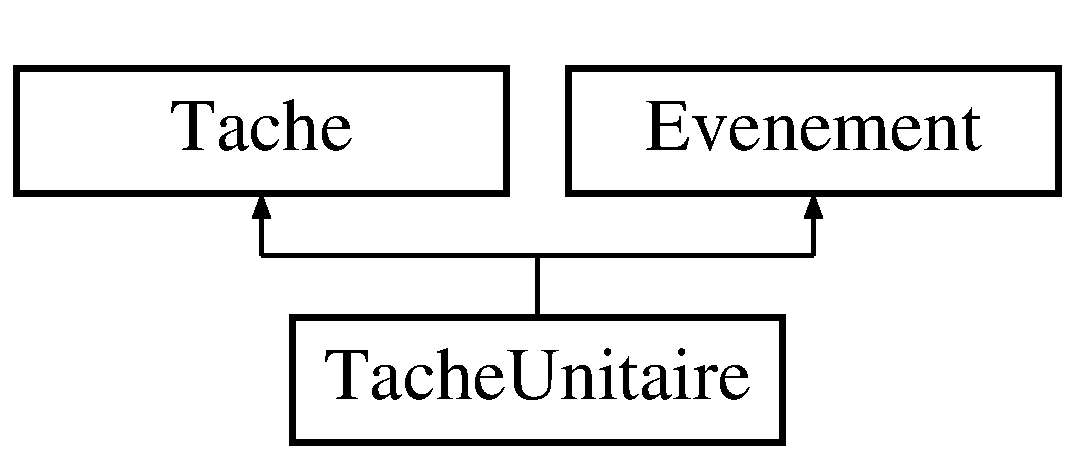
\includegraphics[height=2.000000cm]{class_tache_unitaire}
\end{center}
\end{figure}
\subsection*{Fonctions membres publiques}
\begin{DoxyCompactItemize}
\item 
const Q\+Date\+Time \& \hyperlink{class_tache_unitaire_a931e6c45135ed4cd554826fad8359ff5}{get\+Echeance} () const 
\item 
void \hyperlink{class_tache_unitaire_a4065892def718cee931fe8bdbafa7ffc}{set\+Duree} (const \hyperlink{class_q_time_span}{Q\+Time\+Span} \&d)
\item 
bool \hyperlink{class_tache_unitaire_a93e310a15ded15de3f8cd281120d8b37}{is\+Preemptive} () const override
\item 
void \hyperlink{class_tache_unitaire_abb5fe9e4ca36a2f08b3e8c04555c445d}{set\+Preemptive} (const bool \&b)
\item 
Q\+String \hyperlink{class_tache_unitaire_aa7c4a19559acd6f9267754b611d27cc2}{who\+Am\+I} () const 
\item 
void \hyperlink{class_tache_unitaire_a8f28f8372a319aaee49881487f530a60}{afficher} () const 
\item 
const Q\+String \hyperlink{class_tache_unitaire_af0fbc4b33b3a844dd6a2a1bffde5ec67}{get\+Id} () const 
\end{DoxyCompactItemize}
\subsection*{Amis}
\begin{DoxyCompactItemize}
\item 
\hypertarget{class_tache_unitaire_a59876a285574eb2b160307049a269610}{}class {\bfseries Tache\+Manager}\label{class_tache_unitaire_a59876a285574eb2b160307049a269610}

\item 
\hypertarget{class_tache_unitaire_a46c1844e74be2532f86bf3a09ec141e7}{}class {\bfseries Manager$<$ Tache, Tache\+Manager $>$}\label{class_tache_unitaire_a46c1844e74be2532f86bf3a09ec141e7}

\end{DoxyCompactItemize}
\subsection*{Membres hérités additionnels}


\subsection{Description détaillée}
Une \hyperlink{class_tache_unitaire}{Tache\+Unitaire} est une tâche programmable et composable. Elle ne peut être instanciée que par le biais du \hyperlink{class_tache_manager}{Tache\+Manager}. 

\subsection{Documentation des fonctions membres}
\hypertarget{class_tache_unitaire_a8f28f8372a319aaee49881487f530a60}{}\index{Tache\+Unitaire@{Tache\+Unitaire}!afficher@{afficher}}
\index{afficher@{afficher}!Tache\+Unitaire@{Tache\+Unitaire}}
\subsubsection[{afficher}]{\setlength{\rightskip}{0pt plus 5cm}void Tache\+Unitaire\+::afficher (
\begin{DoxyParamCaption}
{}
\end{DoxyParamCaption}
) const\hspace{0.3cm}{\ttfamily [virtual]}}\label{class_tache_unitaire_a8f28f8372a319aaee49881487f530a60}
La méthode \hyperlink{class_tache_unitaire_a8f28f8372a319aaee49881487f530a60}{afficher()} permet d\textquotesingle{}afficher en mode debug les attributs de la tâche.

Réimplémentée à partir de \hyperlink{class_tache_aa56e1690299f9b6892d21e10df7768b0}{Tache}.

\hypertarget{class_tache_unitaire_a931e6c45135ed4cd554826fad8359ff5}{}\index{Tache\+Unitaire@{Tache\+Unitaire}!get\+Echeance@{get\+Echeance}}
\index{get\+Echeance@{get\+Echeance}!Tache\+Unitaire@{Tache\+Unitaire}}
\subsubsection[{get\+Echeance}]{\setlength{\rightskip}{0pt plus 5cm}const Q\+Date\+Time\& Tache\+Unitaire\+::get\+Echeance (
\begin{DoxyParamCaption}
{}
\end{DoxyParamCaption}
) const\hspace{0.3cm}{\ttfamily [inline]}}\label{class_tache_unitaire_a931e6c45135ed4cd554826fad8359ff5}
Renvoie l\textquotesingle{}écheance de la tache. \hypertarget{class_tache_unitaire_af0fbc4b33b3a844dd6a2a1bffde5ec67}{}\index{Tache\+Unitaire@{Tache\+Unitaire}!get\+Id@{get\+Id}}
\index{get\+Id@{get\+Id}!Tache\+Unitaire@{Tache\+Unitaire}}
\subsubsection[{get\+Id}]{\setlength{\rightskip}{0pt plus 5cm}const Q\+String Tache\+Unitaire\+::get\+Id (
\begin{DoxyParamCaption}
{}
\end{DoxyParamCaption}
) const\hspace{0.3cm}{\ttfamily [inline]}, {\ttfamily [virtual]}}\label{class_tache_unitaire_af0fbc4b33b3a844dd6a2a1bffde5ec67}
Renvoie l\textquotesingle{}identificateur de la tache. 

Implémente \hyperlink{class_evenement}{Evenement}.

\hypertarget{class_tache_unitaire_a93e310a15ded15de3f8cd281120d8b37}{}\index{Tache\+Unitaire@{Tache\+Unitaire}!is\+Preemptive@{is\+Preemptive}}
\index{is\+Preemptive@{is\+Preemptive}!Tache\+Unitaire@{Tache\+Unitaire}}
\subsubsection[{is\+Preemptive}]{\setlength{\rightskip}{0pt plus 5cm}bool Tache\+Unitaire\+::is\+Preemptive (
\begin{DoxyParamCaption}
{}
\end{DoxyParamCaption}
) const\hspace{0.3cm}{\ttfamily [inline]}, {\ttfamily [override]}, {\ttfamily [virtual]}}\label{class_tache_unitaire_a93e310a15ded15de3f8cd281120d8b37}
Renvoie vrai si la tâche est préemptive, faux sinon. 

Implémente \hyperlink{class_evenement}{Evenement}.

\hypertarget{class_tache_unitaire_a4065892def718cee931fe8bdbafa7ffc}{}\index{Tache\+Unitaire@{Tache\+Unitaire}!set\+Duree@{set\+Duree}}
\index{set\+Duree@{set\+Duree}!Tache\+Unitaire@{Tache\+Unitaire}}
\subsubsection[{set\+Duree}]{\setlength{\rightskip}{0pt plus 5cm}void Tache\+Unitaire\+::set\+Duree (
\begin{DoxyParamCaption}
\item[{const {\bf Q\+Time\+Span} \&}]{d}
\end{DoxyParamCaption}
)\hspace{0.3cm}{\ttfamily [inline]}, {\ttfamily [virtual]}}\label{class_tache_unitaire_a4065892def718cee931fe8bdbafa7ffc}
Met à jour la durée de la tâche en prenant en compte le fait qu\textquotesingle{}elle soit est préemptive ou non. 

Réimplémentée à partir de \hyperlink{class_evenement_a8e7e4eb2ec7352a1bf5a63df42c193c6}{Evenement}.

\hypertarget{class_tache_unitaire_abb5fe9e4ca36a2f08b3e8c04555c445d}{}\index{Tache\+Unitaire@{Tache\+Unitaire}!set\+Preemptive@{set\+Preemptive}}
\index{set\+Preemptive@{set\+Preemptive}!Tache\+Unitaire@{Tache\+Unitaire}}
\subsubsection[{set\+Preemptive}]{\setlength{\rightskip}{0pt plus 5cm}void Tache\+Unitaire\+::set\+Preemptive (
\begin{DoxyParamCaption}
\item[{const bool \&}]{b}
\end{DoxyParamCaption}
)\hspace{0.3cm}{\ttfamily [inline]}}\label{class_tache_unitaire_abb5fe9e4ca36a2f08b3e8c04555c445d}
Met à jour la préemptivité de la tâche. \hypertarget{class_tache_unitaire_aa7c4a19559acd6f9267754b611d27cc2}{}\index{Tache\+Unitaire@{Tache\+Unitaire}!who\+Am\+I@{who\+Am\+I}}
\index{who\+Am\+I@{who\+Am\+I}!Tache\+Unitaire@{Tache\+Unitaire}}
\subsubsection[{who\+Am\+I}]{\setlength{\rightskip}{0pt plus 5cm}Q\+String Tache\+Unitaire\+::who\+Am\+I (
\begin{DoxyParamCaption}
{}
\end{DoxyParamCaption}
) const\hspace{0.3cm}{\ttfamily [inline]}, {\ttfamily [virtual]}}\label{class_tache_unitaire_aa7c4a19559acd6f9267754b611d27cc2}
Renvoie le type de tâche, ici \char`\"{}tâche\+\_\+unitaire\char`\"{}. 

Implémente \hyperlink{class_evenement}{Evenement}.



La documentation de cette classe a été générée à partir des fichiers suivants \+:\begin{DoxyCompactItemize}
\item 
evenement.\+h\item 
evenement.\+cpp\end{DoxyCompactItemize}

\hypertarget{class_t_i_m_e_1_1_time_exception}{}\section{Référence de la classe T\+I\+M\+E\+:\+:Time\+Exception}
\label{class_t_i_m_e_1_1_time_exception}\index{T\+I\+M\+E\+::\+Time\+Exception@{T\+I\+M\+E\+::\+Time\+Exception}}


Classe permettant de gérer les exceptions des classes du namespace T\+I\+M\+E.  




{\ttfamily \#include $<$timing.\+h$>$}

\subsection*{Fonctions membres publiques}
\begin{DoxyCompactItemize}
\item 
\hypertarget{class_t_i_m_e_1_1_time_exception_a08502d82065dd79b27cd954b45f4d5c7}{}\hyperlink{class_t_i_m_e_1_1_time_exception_a08502d82065dd79b27cd954b45f4d5c7}{Time\+Exception} (const std\+::string \&m)\label{class_t_i_m_e_1_1_time_exception_a08502d82065dd79b27cd954b45f4d5c7}

\begin{DoxyCompactList}\small\item\em Constructeur à partir d\textquotesingle{}une string. \end{DoxyCompactList}\item 
\hypertarget{class_t_i_m_e_1_1_time_exception_ad86c212253ea1b8654f4cae34611d634}{}const std\+::string \& {\bfseries Get\+Info} () const \label{class_t_i_m_e_1_1_time_exception_ad86c212253ea1b8654f4cae34611d634}

\end{DoxyCompactItemize}


\subsection{Description détaillée}
Classe permettant de gérer les exceptions des classes du namespace T\+I\+M\+E. 

La documentation de cette classe a été générée à partir du fichier suivant \+:\begin{DoxyCompactItemize}
\item 
timing.\+h\end{DoxyCompactItemize}

\hypertarget{classvue_globale}{}\section{Référence de la classe vue\+Globale}
\label{classvue_globale}\index{vue\+Globale@{vue\+Globale}}


Fenêtre de visualisation globale à l\textquotesingle{}aide d\textquotesingle{}un Tree\+View.  




{\ttfamily \#include $<$vueglobale.\+h$>$}

Graphe d\textquotesingle{}héritage de vue\+Globale\+:\begin{figure}[H]
\begin{center}
\leavevmode
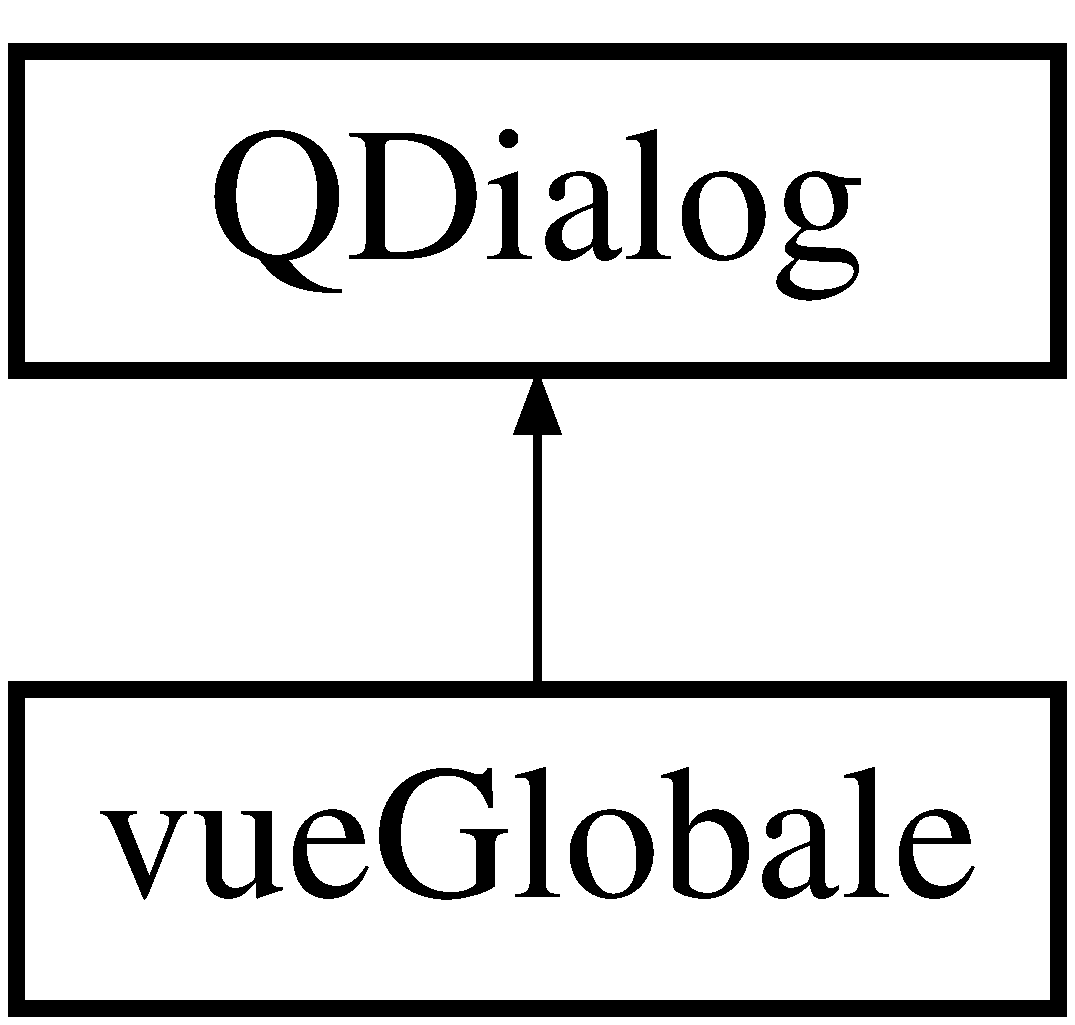
\includegraphics[height=2.000000cm]{classvue_globale}
\end{center}
\end{figure}
\subsection*{Types publics}
\begin{DoxyCompactItemize}
\item 
\hypertarget{classvue_globale_af10a90ecd40a8aead21f78a2cdb0d39a}{}enum {\bfseries Type} \{ {\bfseries P\+R\+O\+J\+E\+T}, 
{\bfseries I\+D\+E\+N\+T\+I\+F\+I\+C\+A\+T\+E\+U\+R}, 
{\bfseries P\+R\+O\+G\+R\+A\+M\+M\+A\+T\+I\+O\+N}, 
{\bfseries D\+U\+R\+E\+E}
 \}\label{classvue_globale_af10a90ecd40a8aead21f78a2cdb0d39a}

\end{DoxyCompactItemize}
\subsection*{Fonctions membres publiques}
\begin{DoxyCompactItemize}
\item 
\hypertarget{classvue_globale_a6bff14519ecc6449dd50c0a64fc1027b}{}{\bfseries vue\+Globale} (Q\+Widget $\ast$parent=0)\label{classvue_globale_a6bff14519ecc6449dd50c0a64fc1027b}

\item 
\hypertarget{classvue_globale_a644d1fdbb22daebc35dc7e530b66166b}{}Q\+Tree\+Widget\+Item $\ast$ {\bfseries insert\+Projet} (const \hyperlink{class_projet}{Projet} \&p)\label{classvue_globale_a644d1fdbb22daebc35dc7e530b66166b}

\item 
\hypertarget{classvue_globale_a7943572f94eefd6018be233f563029f4}{}Q\+Tree\+Widget\+Item $\ast$ {\bfseries insert\+Item} (const Q\+String \&nom, Q\+Tree\+Widget\+Item $\ast$parent)\label{classvue_globale_a7943572f94eefd6018be233f563029f4}

\item 
\hypertarget{classvue_globale_ae27c01d8d51aa88a6f181ea9f89bdd71}{}Q\+Tree\+Widget\+Item $\ast$ {\bfseries insert\+Item} (const Q\+String \&nom, const Q\+String \&duree, Q\+Tree\+Widget\+Item $\ast$parent)\label{classvue_globale_ae27c01d8d51aa88a6f181ea9f89bdd71}

\item 
\hypertarget{classvue_globale_a28f35c6d40e0beb35c306a639f2be5e0}{}Q\+Tree\+Widget\+Item $\ast$ {\bfseries insert\+Item} (const Q\+String \&nom, const Q\+String \&duree, const Q\+String \&prog, Q\+Tree\+Widget\+Item $\ast$parent)\label{classvue_globale_a28f35c6d40e0beb35c306a639f2be5e0}

\end{DoxyCompactItemize}


\subsection{Description détaillée}
Fenêtre de visualisation globale à l\textquotesingle{}aide d\textquotesingle{}un Tree\+View. 

La documentation de cette classe a été générée à partir des fichiers suivants \+:\begin{DoxyCompactItemize}
\item 
G\+U\+I/vueglobale.\+h\item 
G\+U\+I/vueglobale.\+cpp\end{DoxyCompactItemize}

\hypertarget{class_x_m_l}{}\section{Référence de la classe X\+M\+L}
\label{class_x_m_l}\index{X\+M\+L@{X\+M\+L}}


La classe \hyperlink{class_x_m_l}{X\+M\+L} est un \hyperlink{class_format}{Format} et permet d\textquotesingle{}exporter l\textquotesingle{}ensemble des données du calendrier sous forme \hyperlink{class_x_m_l}{X\+M\+L}.  




{\ttfamily \#include $<$import-\/export.\+h$>$}

Graphe d\textquotesingle{}héritage de X\+M\+L\+:\begin{figure}[H]
\begin{center}
\leavevmode
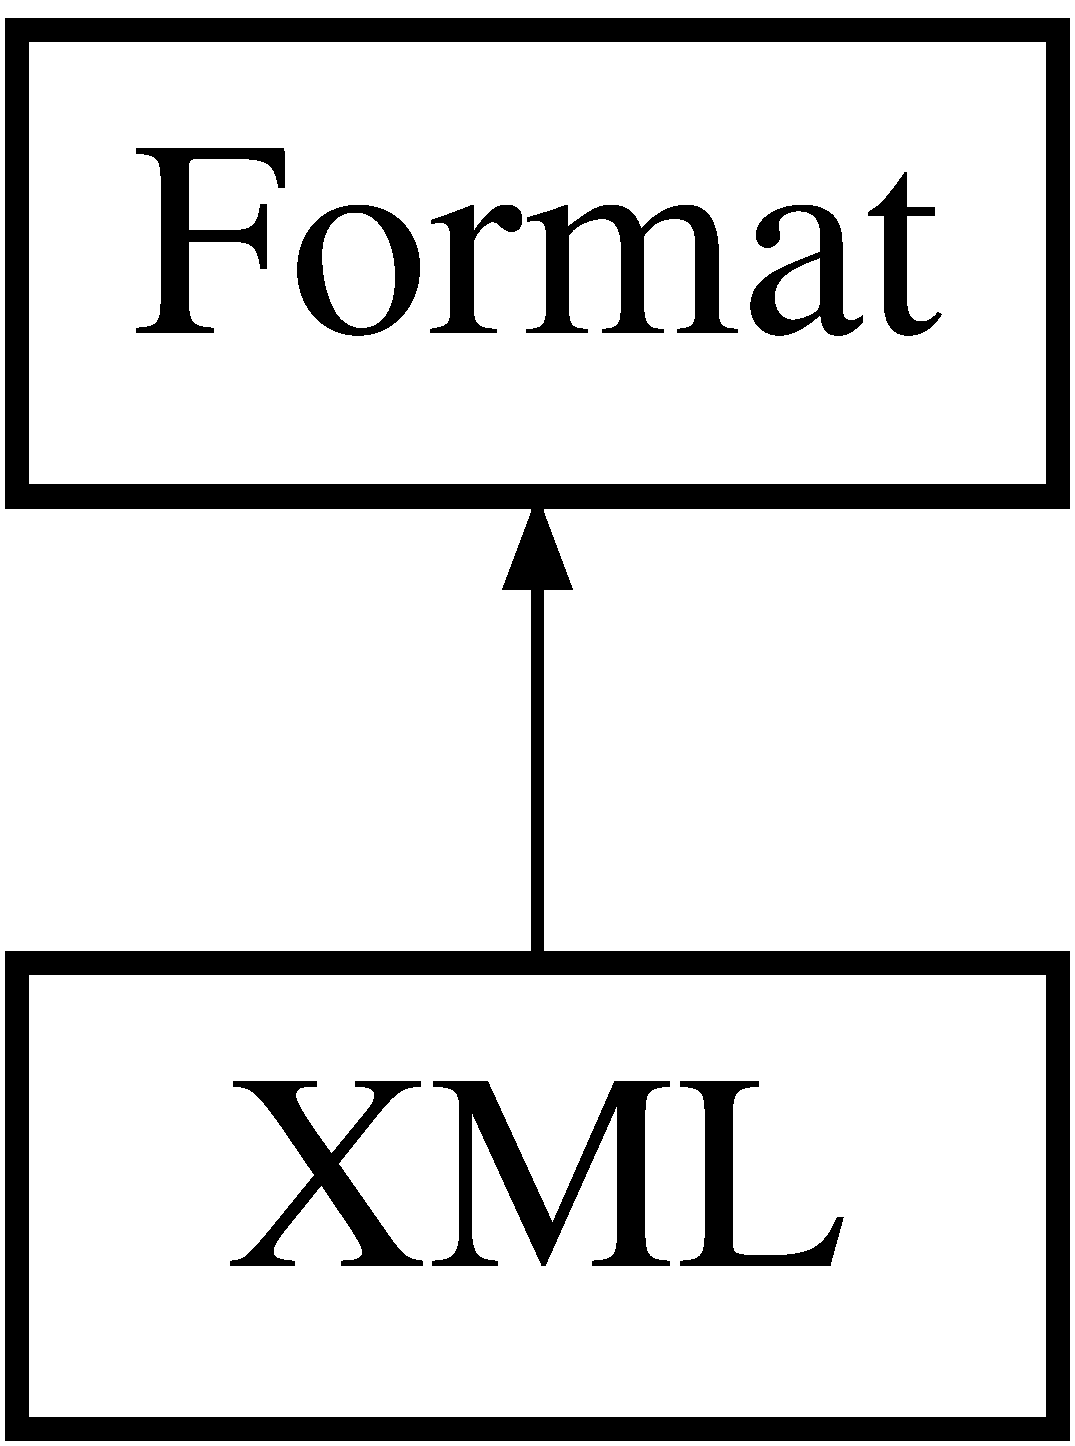
\includegraphics[height=2.000000cm]{class_x_m_l}
\end{center}
\end{figure}
\subsection*{Fonctions membres publiques}
\begin{DoxyCompactItemize}
\item 
void \hyperlink{class_x_m_l_a0c2f3b489419670e42e6cb3b5a99d685}{save} () const override
\item 
void \hyperlink{class_x_m_l_a4d293b9b95938449b0eb789cc93d9b50}{save\+Projet} (Q\+Xml\+Stream\+Writer \&stream, const \hyperlink{class_projet}{Projet} \&proj) const 
\item 
void \hyperlink{class_x_m_l_acd2ed06f43002937540f02db3edd5119}{save\+Tache} (Q\+Xml\+Stream\+Writer \&stream, const \hyperlink{class_tache}{Tache} \&tache) const 
\item 
void \hyperlink{class_x_m_l_acedd44046fabe1b5e92a67d5a92bc577}{save\+Activite} (Q\+Xml\+Stream\+Writer \&stream, const \hyperlink{class_activite}{Activite} \&act) const 
\item 
void \hyperlink{class_x_m_l_a954c040930e567a46c2390f0188f273d}{save\+Programmation} (Q\+Xml\+Stream\+Writer \&stream, const \hyperlink{class_programmation}{Programmation} \&prog) const 
\item 
void \hyperlink{class_x_m_l_ad0ece286ff5262a63e68e08e2878b0c8}{save\+Precedence} (Q\+Xml\+Stream\+Writer \&stream, const \hyperlink{class_precedence}{Precedence} \&prec) const 
\item 
void \hyperlink{class_x_m_l_aba46159218c520cdc783654b34a2c0dd}{load} () const override
\item 
void \hyperlink{class_x_m_l_a67683ccfd45dcc4aa18317fefcf723fd}{load\+Projet} (Q\+Xml\+Stream\+Reader \&stream) const 
\item 
\hyperlink{class_tache}{Tache} \& \hyperlink{class_x_m_l_a0b5ebfcd1601f9353d9d13f8290e7319}{load\+Tache} (Q\+Xml\+Stream\+Reader \&stream) const 
\item 
void \hyperlink{class_x_m_l_a554eb55c0c69dbc3045615d0ab68ab1d}{load\+Activite} (Q\+Xml\+Stream\+Reader \&stream) const 
\item 
void \hyperlink{class_x_m_l_a0f2858b84a734c0238d4478df89ce170}{load\+Programmation} (Q\+Xml\+Stream\+Reader \&stream) const 
\item 
void \hyperlink{class_x_m_l_a0593dfc3350675f6da3098ac68bb060d}{load\+Precedence} (Q\+Xml\+Stream\+Reader \&stream) const 
\end{DoxyCompactItemize}
\subsection*{Fonctions membres publiques statiques}
\begin{DoxyCompactItemize}
\item 
static \hyperlink{class_x_m_l}{X\+M\+L} \& \hyperlink{class_x_m_l_aa2d6c4ab68ae45a0cbb71d3baa67a119}{get\+Instance} (const Q\+String \&p=\char`\"{}auto-\/save.\+xml\char`\"{})
\item 
static void \hyperlink{class_x_m_l_aa636b752f30ee85554a88b29687deed7}{free\+Instance} ()
\end{DoxyCompactItemize}
\subsection*{Membres hérités additionnels}


\subsection{Description détaillée}
La classe \hyperlink{class_x_m_l}{X\+M\+L} est un \hyperlink{class_format}{Format} et permet d\textquotesingle{}exporter l\textquotesingle{}ensemble des données du calendrier sous forme \hyperlink{class_x_m_l}{X\+M\+L}. 

\subsection{Documentation des fonctions membres}
\hypertarget{class_x_m_l_aa636b752f30ee85554a88b29687deed7}{}\index{X\+M\+L@{X\+M\+L}!free\+Instance@{free\+Instance}}
\index{free\+Instance@{free\+Instance}!X\+M\+L@{X\+M\+L}}
\subsubsection[{free\+Instance}]{\setlength{\rightskip}{0pt plus 5cm}void X\+M\+L\+::free\+Instance (
\begin{DoxyParamCaption}
{}
\end{DoxyParamCaption}
)\hspace{0.3cm}{\ttfamily [static]}}\label{class_x_m_l_aa636b752f30ee85554a88b29687deed7}
Libère l\textquotesingle{}instance de la stratégie \hyperlink{class_x_m_l}{X\+M\+L} et entraine sa désallocation mémoire. \hypertarget{class_x_m_l_aa2d6c4ab68ae45a0cbb71d3baa67a119}{}\index{X\+M\+L@{X\+M\+L}!get\+Instance@{get\+Instance}}
\index{get\+Instance@{get\+Instance}!X\+M\+L@{X\+M\+L}}
\subsubsection[{get\+Instance}]{\setlength{\rightskip}{0pt plus 5cm}{\bf X\+M\+L} \& X\+M\+L\+::get\+Instance (
\begin{DoxyParamCaption}
\item[{const Q\+String \&}]{p = {\ttfamily \char`\"{}auto-\/save.xml\char`\"{}}}
\end{DoxyParamCaption}
)\hspace{0.3cm}{\ttfamily [static]}}\label{class_x_m_l_aa2d6c4ab68ae45a0cbb71d3baa67a119}
Instancie un objet de la classe \hyperlink{class_x_m_l}{X\+M\+L} si aucune instanciation n\textquotesingle{}a été faite au préalable, et retourne sa référence. \hypertarget{class_x_m_l_aba46159218c520cdc783654b34a2c0dd}{}\index{X\+M\+L@{X\+M\+L}!load@{load}}
\index{load@{load}!X\+M\+L@{X\+M\+L}}
\subsubsection[{load}]{\setlength{\rightskip}{0pt plus 5cm}void X\+M\+L\+::load (
\begin{DoxyParamCaption}
{}
\end{DoxyParamCaption}
) const\hspace{0.3cm}{\ttfamily [override]}, {\ttfamily [virtual]}}\label{class_x_m_l_aba46159218c520cdc783654b34a2c0dd}
Effectue le chargement total de l\textquotesingle{}ensemble des informations du calendrier stockés dans un fichier \hyperlink{class_x_m_l}{X\+M\+L}.
\begin{DoxyItemize}
\item Projets
\item Tâches
\item Activités
\item Précédences
\item Programmations 
\end{DoxyItemize}

Implémente \hyperlink{class_format}{Format}.

\hypertarget{class_x_m_l_a554eb55c0c69dbc3045615d0ab68ab1d}{}\index{X\+M\+L@{X\+M\+L}!load\+Activite@{load\+Activite}}
\index{load\+Activite@{load\+Activite}!X\+M\+L@{X\+M\+L}}
\subsubsection[{load\+Activite}]{\setlength{\rightskip}{0pt plus 5cm}void X\+M\+L\+::load\+Activite (
\begin{DoxyParamCaption}
\item[{Q\+Xml\+Stream\+Reader \&}]{stream}
\end{DoxyParamCaption}
) const}\label{class_x_m_l_a554eb55c0c69dbc3045615d0ab68ab1d}
Charge toutes les activités au sein du \hyperlink{class_activite_manager}{Activite\+Manager} depuis le stream de type Q\+Xml\+Stream\+Reader. \hypertarget{class_x_m_l_a0593dfc3350675f6da3098ac68bb060d}{}\index{X\+M\+L@{X\+M\+L}!load\+Precedence@{load\+Precedence}}
\index{load\+Precedence@{load\+Precedence}!X\+M\+L@{X\+M\+L}}
\subsubsection[{load\+Precedence}]{\setlength{\rightskip}{0pt plus 5cm}void X\+M\+L\+::load\+Precedence (
\begin{DoxyParamCaption}
\item[{Q\+Xml\+Stream\+Reader \&}]{stream}
\end{DoxyParamCaption}
) const}\label{class_x_m_l_a0593dfc3350675f6da3098ac68bb060d}
Charge toutes les précédences au sein du \hyperlink{class_precedence_manager}{Precedence\+Manager} depuis le stream de type Q\+Xml\+Stream\+Reader. \hypertarget{class_x_m_l_a0f2858b84a734c0238d4478df89ce170}{}\index{X\+M\+L@{X\+M\+L}!load\+Programmation@{load\+Programmation}}
\index{load\+Programmation@{load\+Programmation}!X\+M\+L@{X\+M\+L}}
\subsubsection[{load\+Programmation}]{\setlength{\rightskip}{0pt plus 5cm}void X\+M\+L\+::load\+Programmation (
\begin{DoxyParamCaption}
\item[{Q\+Xml\+Stream\+Reader \&}]{stream}
\end{DoxyParamCaption}
) const}\label{class_x_m_l_a0f2858b84a734c0238d4478df89ce170}
Charge toutes les programmations au sein du \hyperlink{class_programmation_manager}{Programmation\+Manager} depuis le stream de type Q\+Xml\+Stream\+Reader. \hypertarget{class_x_m_l_a67683ccfd45dcc4aa18317fefcf723fd}{}\index{X\+M\+L@{X\+M\+L}!load\+Projet@{load\+Projet}}
\index{load\+Projet@{load\+Projet}!X\+M\+L@{X\+M\+L}}
\subsubsection[{load\+Projet}]{\setlength{\rightskip}{0pt plus 5cm}void X\+M\+L\+::load\+Projet (
\begin{DoxyParamCaption}
\item[{Q\+Xml\+Stream\+Reader \&}]{stream}
\end{DoxyParamCaption}
) const}\label{class_x_m_l_a67683ccfd45dcc4aa18317fefcf723fd}
Charge tous les projets au sein du \hyperlink{class_projet_manager}{Projet\+Manager} depuis le stream de type Q\+Xml\+Stream\+Reader. \hypertarget{class_x_m_l_a0b5ebfcd1601f9353d9d13f8290e7319}{}\index{X\+M\+L@{X\+M\+L}!load\+Tache@{load\+Tache}}
\index{load\+Tache@{load\+Tache}!X\+M\+L@{X\+M\+L}}
\subsubsection[{load\+Tache}]{\setlength{\rightskip}{0pt plus 5cm}{\bf Tache} \& X\+M\+L\+::load\+Tache (
\begin{DoxyParamCaption}
\item[{Q\+Xml\+Stream\+Reader \&}]{stream}
\end{DoxyParamCaption}
) const}\label{class_x_m_l_a0b5ebfcd1601f9353d9d13f8290e7319}
Charge toutes les tâches au sein du \hyperlink{class_tache_manager}{Tache\+Manager} depuis le stream de type Q\+Xml\+Stream\+Reader. \hypertarget{class_x_m_l_a0c2f3b489419670e42e6cb3b5a99d685}{}\index{X\+M\+L@{X\+M\+L}!save@{save}}
\index{save@{save}!X\+M\+L@{X\+M\+L}}
\subsubsection[{save}]{\setlength{\rightskip}{0pt plus 5cm}void X\+M\+L\+::save (
\begin{DoxyParamCaption}
{}
\end{DoxyParamCaption}
) const\hspace{0.3cm}{\ttfamily [override]}, {\ttfamily [virtual]}}\label{class_x_m_l_a0c2f3b489419670e42e6cb3b5a99d685}
Effectue la sauvegarde totale de l\textquotesingle{}ensemble des informations du calendrier au sein d\textquotesingle{}un fichier \hyperlink{class_x_m_l}{X\+M\+L}\+:
\begin{DoxyItemize}
\item Projets\+: en appellant \hyperlink{class_x_m_l_a4d293b9b95938449b0eb789cc93d9b50}{save\+Projet()}
\item Tâches\+: en appellant \hyperlink{class_x_m_l_acd2ed06f43002937540f02db3edd5119}{save\+Tache()}
\item Activités\+: en appellant \hyperlink{class_x_m_l_acedd44046fabe1b5e92a67d5a92bc577}{save\+Activite()}
\item Précédences\+: en appellant \hyperlink{class_x_m_l_ad0ece286ff5262a63e68e08e2878b0c8}{save\+Precedence()}
\item Programmations\+: en appellant \hyperlink{class_x_m_l_a954c040930e567a46c2390f0188f273d}{save\+Programmation()}
\end{DoxyItemize}

Pour sauvegarder chaque item, la méthode \hyperlink{class_x_m_l_a0c2f3b489419670e42e6cb3b5a99d685}{save()} parcourt les différents manager à l\textquotesingle{}aide d\textquotesingle{}un iterator. 

Implémente \hyperlink{class_format}{Format}.

\hypertarget{class_x_m_l_acedd44046fabe1b5e92a67d5a92bc577}{}\index{X\+M\+L@{X\+M\+L}!save\+Activite@{save\+Activite}}
\index{save\+Activite@{save\+Activite}!X\+M\+L@{X\+M\+L}}
\subsubsection[{save\+Activite}]{\setlength{\rightskip}{0pt plus 5cm}void X\+M\+L\+::save\+Activite (
\begin{DoxyParamCaption}
\item[{Q\+Xml\+Stream\+Writer \&}]{stream, }
\item[{const {\bf Activite} \&}]{act}
\end{DoxyParamCaption}
) const}\label{class_x_m_l_acedd44046fabe1b5e92a67d5a92bc577}
Sauvegarde l\textquotesingle{}activité dans le stream Q\+Xml\+Stream\+Writer, tous deux passés en paramètre. \hypertarget{class_x_m_l_ad0ece286ff5262a63e68e08e2878b0c8}{}\index{X\+M\+L@{X\+M\+L}!save\+Precedence@{save\+Precedence}}
\index{save\+Precedence@{save\+Precedence}!X\+M\+L@{X\+M\+L}}
\subsubsection[{save\+Precedence}]{\setlength{\rightskip}{0pt plus 5cm}void X\+M\+L\+::save\+Precedence (
\begin{DoxyParamCaption}
\item[{Q\+Xml\+Stream\+Writer \&}]{stream, }
\item[{const {\bf Precedence} \&}]{prec}
\end{DoxyParamCaption}
) const}\label{class_x_m_l_ad0ece286ff5262a63e68e08e2878b0c8}
Sauvegarde la précédence dans le stream Q\+Xml\+Stream\+Writer, tous deux passés en paramètre. \hypertarget{class_x_m_l_a954c040930e567a46c2390f0188f273d}{}\index{X\+M\+L@{X\+M\+L}!save\+Programmation@{save\+Programmation}}
\index{save\+Programmation@{save\+Programmation}!X\+M\+L@{X\+M\+L}}
\subsubsection[{save\+Programmation}]{\setlength{\rightskip}{0pt plus 5cm}void X\+M\+L\+::save\+Programmation (
\begin{DoxyParamCaption}
\item[{Q\+Xml\+Stream\+Writer \&}]{stream, }
\item[{const {\bf Programmation} \&}]{prog}
\end{DoxyParamCaption}
) const}\label{class_x_m_l_a954c040930e567a46c2390f0188f273d}
Sauvegarde la programmation dans le stream Q\+Xml\+Stream\+Writer, tous deux passés en paramètre. \hypertarget{class_x_m_l_a4d293b9b95938449b0eb789cc93d9b50}{}\index{X\+M\+L@{X\+M\+L}!save\+Projet@{save\+Projet}}
\index{save\+Projet@{save\+Projet}!X\+M\+L@{X\+M\+L}}
\subsubsection[{save\+Projet}]{\setlength{\rightskip}{0pt plus 5cm}void X\+M\+L\+::save\+Projet (
\begin{DoxyParamCaption}
\item[{Q\+Xml\+Stream\+Writer \&}]{stream, }
\item[{const {\bf Projet} \&}]{proj}
\end{DoxyParamCaption}
) const}\label{class_x_m_l_a4d293b9b95938449b0eb789cc93d9b50}
Sauvegarde le projet dans le stream Q\+Xml\+Stream\+Writer, tous deux passés en paramètre. La méthode sauvegarde également les tâches liées au projet en appelant \hyperlink{class_x_m_l_acd2ed06f43002937540f02db3edd5119}{save\+Tache()}. \hypertarget{class_x_m_l_acd2ed06f43002937540f02db3edd5119}{}\index{X\+M\+L@{X\+M\+L}!save\+Tache@{save\+Tache}}
\index{save\+Tache@{save\+Tache}!X\+M\+L@{X\+M\+L}}
\subsubsection[{save\+Tache}]{\setlength{\rightskip}{0pt plus 5cm}void X\+M\+L\+::save\+Tache (
\begin{DoxyParamCaption}
\item[{Q\+Xml\+Stream\+Writer \&}]{stream, }
\item[{const {\bf Tache} \&}]{tache}
\end{DoxyParamCaption}
) const}\label{class_x_m_l_acd2ed06f43002937540f02db3edd5119}
Sauvegarde la tâche dans le stream Q\+Xml\+Stream\+Writer, tous deux passés en paramètre. 

La documentation de cette classe a été générée à partir des fichiers suivants \+:\begin{DoxyCompactItemize}
\item 
import-\/export.\+h\item 
import-\/export.\+cpp\end{DoxyCompactItemize}

%--- End generated contents ---

% Index
\backmatter
\newpage
\phantomsection
\clearemptydoublepage
\addcontentsline{toc}{chapter}{Index}
\printindex

\end{document}
